% Template adapted from https://github.com/jgm/pandoc-templates/blob/master/default.latex
% To be used with XeLaTex in memoiR
%%%%%%%%%%%%%%%%%%%%%%%%%%%%%%%%%%%%%%%%%%%%%%%%%%%%%%%%%%%%%%%%%%%%%%%%%%%%%%%%%%%%%%%%%

% Options for packages loaded elsewhere
\PassOptionsToPackage{unicode=true}{hyperref}
\PassOptionsToPackage{hyphens}{url}
\PassOptionsToPackage{dvipsnames,svgnames*,x11names*}{xcolor}
% Right to left support


\documentclass[
  11pt,
  american,
  letterpaperpaper,
  extrafontsizes,onecolumn,openright
  ]{memoir}

% Double (or whatever) spacing

% Math
\usepackage{amssymb, amsmath}
% mathspec: arbitrary math fonts
\usepackage{unicode-math}
\defaultfontfeatures{Scale=MatchLowercase}
\defaultfontfeatures[\rmfamily]{Ligatures=TeX,Scale=1}

% Fonts
\usepackage{lmodern}
\usepackage{fontspec}
% Main font
% Specific sanserif font
% Specific monotype font
% Specific math font
% Chinese, Japanese, Corean fonts

% Use upquote for straight quotes in verbatim environments
\usepackage{upquote}
% Use microtype
\usepackage[]{microtype}
\UseMicrotypeSet[protrusion]{basicmath} % disable protrusion for tt fonts

% Verbatim in note

% Color links
\usepackage{xcolor}

% Strikeout

% Necessary for code chunks

% Listings package

% Tables
\usepackage{longtable,booktabs,tabu}
% Fix footnotes in tables (requires footnote package)
\IfFileExists{footnote.sty}{\usepackage{footnote}\makesavenoteenv{longtable}}{}

% Graphics
\usepackage{graphicx,grffile}
\graphicspath{{images/}}
\makeatletter
\def\maxwidth{\ifdim\Gin@nat@width>\linewidth\linewidth\else\Gin@nat@width\fi}
\def\maxheight{\ifdim\Gin@nat@height>\textheight\textheight\else\Gin@nat@height\fi}
\makeatother
% Scale images if necessary, so that they will not overflow the page
% margins by default, and it is still possible to overwrite the defaults
% using explicit options in \includegraphics[width, height, ...]{}
\setkeys{Gin}{width=\maxwidth,height=\maxheight,keepaspectratio}

% Prevent overfull lines
\setlength{\emergencystretch}{3em}  
\providecommand{\tightlist}{%
  \setlength{\itemsep}{0pt}\setlength{\parskip}{0pt}}

% Number sections for memoir (secnumdepth counter is ignored)
\setsecnumdepth{section}

% Set default figure placement to htbp
\makeatletter
\def\fps@figure{htbp}
\makeatother

% Spacing in lists
\usepackage{enumitem}

% Polyglossia
\usepackage{polyglossia}
\setmainlanguage{en-US}
\setotherlanguage{fr-FR}
\setotherlanguage{it}

% localized quotes
\usepackage[strict,autostyle]{csquotes}

% BibLaTeX
\usepackage[backend=biber,style=authoryear-ibid,isbn=false,backref=true,giveninits=true,uniquename=init,maxcitenames=2,maxbibnames=150,sorting=nyt,sortcites=false]{biblatex}
\addbibresource{references.bib}

% cslreferences environment required by pandoc > 2.7



%%%%%%%%%%%%%%%%%%%%%%%%%%%%%%%%%%%%%%%%%%%%%%%%%%%%%%%%%%
% memoiR format

% Chapter Summary environment 
\usepackage[tikz]{bclogo}
\newenvironment{Summary}
  {\begin{bclogo}[logo=\bctrombone, noborder=true, couleur=lightgray!50]{}\parindent0pt}
  {\end{bclogo}}
% Syntax:
%
%```{block, type='Summary'}
% Deliver message here.
% ```

% scriptsize code 
\let\oldverbatim\verbatim
\def\verbatim{\oldverbatim\scriptsize}
% Applies to code blocks and R code results
% code chunk options size='scriptsize' applies only to R code and results
% if the code chunk sets a different size, \def\verbatim{...} is prioritary for code results 


% memoiR dalef3 chapter style 
% https://ctan.crest.fr/tex-archive/info/latex-samples/MemoirChapStyles/MemoirChapStyles.pdf
\usepackage{soul}
\definecolor{nicered}{rgb}{0,.294,.561}
\makeatletter
\newlength\dlf@normtxtw
\setlength\dlf@normtxtw{\textwidth}
\def\myhelvetfont{\def\sfdefault{mdput}}
\newsavebox{\feline@chapter}
\newcommand\feline@chapter@marker[1][4cm]{%
  \sbox\feline@chapter{%
    \resizebox{!}{#1}{\fboxsep=1pt%
	  \colorbox{nicered}{\color{white}\bfseries\sffamily\thechapter}%
	}}%
  \rotatebox{90}{%
    \resizebox{%
	  \heightof{\usebox{\feline@chapter}}+\depthof{\usebox{\feline@chapter}}}%
	{!}{\scshape\so\@chapapp}}\quad%
  \raisebox{\depthof{\usebox{\feline@chapter}}}{\usebox{\feline@chapter}}%
 }
\newcommand\feline@chm[1][4cm]{%
  \sbox\feline@chapter{\feline@chapter@marker[#1]}%
  \makebox[0pt][l]{% aka \rlap
    \makebox[1cm][r]{\usebox\feline@chapter}%
  }}
\makechapterstyle{daleif1}{
  \renewcommand\chapnamefont{\normalfont\Large\scshape\raggedleft\so}
  \renewcommand\chaptitlefont{\normalfont\huge\bfseries\scshape\color{nicered}}
  \renewcommand\chapternamenum{}
  \renewcommand\printchaptername{}
  \renewcommand\printchapternum{\null\hfill\feline@chm[2.5cm]\par}
  \renewcommand\afterchapternum{\par\vskip\midchapskip}
  \renewcommand\printchaptertitle[1]{\chaptitlefont\raggedleft ##1\par}
}
\makeatother


% Layout
%%%%%%%%%%%%%%%%%%%%%%%%%%%%%%%%%%%%%%%%%%%%%%%%%%%%%%%%%%

% Based on memoir, style companion
\newcommand{\MemoirChapStyle}{daleif1}
\newcommand{\MemoirPageStyle}{Ruled}

% Space between paragraphs
\usepackage{parskip}
  \abnormalparskip{3pt}

% Adjust margin paragraphs vertical position
\usepackage{marginfix}


% Margins
%%%%%%%%%%%%%%%%%%%%%%%%%%%%%%%%%%%%%%%

% allow use of '-',+','/' ans '*' to make simple length computation
\usepackage{calc}

% Full-width figures utilities
\newlength\widthw % full width
\newlength{\rf}
\newcommand*{\definesHSpace}{
  \strictpagecheck % slower but efficient detection of odd/even pages
  \checkoddpage
  \ifoddpage
  \setlength{\rf}{0mm}
  \else
  \setlength{\rf}{\marginparsep+\marginparwidth}
  \fi
}

\makeatletter
% 1" margins for the front matter.
\newcommand*{\SmallMargins}{
  \setlrmarginsandblock{1.5in}{1.5in}{*}
  \setmarginnotes{0.1in}{0.1in}{0.1in}
 \setulmarginsandblock{1.5in}{1in}{*}
  \checkandfixthelayout
  \ch@ngetext
  \clearpage
  \setlength{\widthw}{\textwidth+\marginparsep+\marginparwidth}
  \footnotesatfoot
  \chapterstyle{\MemoirChapStyle}  % Chapter and page styles must be recalled
  \pagestyle{\MemoirPageStyle}
}

% 3" outer margin for the main matter
\newcommand{\LargeMargins}{\SmallMargins}
\makeatother

% Figure captions and footnotes in outer margins


% Local toc
%%%%%%%%%%%%%%%%%%%%%%%%%%%%%%%%%%%%%%%%%%%%%%%%%%%%%%%%%%

\usepackage{titletoc}
\newcommand{\toc}[1]{%
  \startcontents[chapters]%
  \printcontents[chapters]{}{1}[#1]{}%
  ~\newline%
}


% Text boxes
%%%%%%%%%%%%%%%%%%%%%%%%%%%%%%%%%%%%%%%%%%%%%%%%%%%%%%%%%%

% Define a style for mdframed boxes
\mdfdefinestyle{boxstyle}{
	skipabove=1.5\topskip,
	skipbelow=.5\topskip,
	rightmargin=0pt,
	leftmargin=0pt,
	innerrightmargin=7pt,
	innerleftmargin=7pt,
	topline=false,
	bottomline=false,
	rightline=false,
	leftline=false,
	frametitlerule=true,
	linecolor=black,
	fontcolor=black,
	frametitlealignment=\noindent
}


% Main title page with filigrane
%%%%%%%%%%%%%%%%%%%%%%%%%%%%%%%%%%%%%%%%%%%%%%%%%%%%%%%%%%


% Clear page and open an even one (\clearpage opens an odd one)
\newcommand{\evenpage}{
  \clearpage
  \strictpagecheck % slower but efficient detection of odd/even pages
  \checkoddpage
  \ifoddpage
    \thispagestyle{empty}
    ~\\ % Print a character or the page will not exist
    \newpage
  \else
    % do nothing
  \fi
}


%% PDF title page to insert
%%%%%%%%%%%%%%%%%%%%%%%%%%%%%%%%%%%%%%%%%%%%%%%%%%%%%%%%%%

\usepackage{pdfpages}


%% Bibliography
%%%%%%%%%%%%%%%%%%%%%%%%%%%%%%%%%%%%%%%%%%%%%%%%%%%%%%%%%%

% Repeated citation as author-year-title instead of author-title (modification of footcite:note in verbose-inote.cbx)

%% Table of Contents
%%%%%%%%%%%%%%%%%%%%%%%%%%%%%%%%%%%%%%%%%%%%%%%%%%%%%%%%%%

% fix the typesetting of the part number
\renewcommand\partnumberlinebox[2]{#2\ ---\ }


% Fonts
%%%%%%%%%%%%%%%%%%%%%%%%%%%%%%%%%%%%%%%%%%%%%%%%%%%%%%%%%%


% Hyperref comes last
%%%%%%%%%%%%%%%%%%%%%%%%%%%%%%%%%%%%%%%%%%%%%%%%%%%%%%%%%%

\usepackage{hyperref}
\hypersetup{
  pdftitle={Getting Started at the JBJ},
  pdfauthor={Timothy J. Gibbons},
  colorlinks=true,
  linkcolor=Maroon,
  citecolor=Blue,
  urlcolor=blue,
  breaklinks=true}

% Don't use monospace font for urls
\urlstyle{same}


% Title, author, date from YAML to LaTeX
%%%%%%%%%%%%%%%%%%%%%%%%%%%%%%%%%%%%%%%%%%%%%%%%%%%%%%%%%%

\title{Getting Started at the JBJ}

\author{Timothy J. Gibbons}

\date{}


% Include headers (preamble.tex) here
%%%%%%%%%%%%%%%%%%%%%%%%%%%%%%%%%%%%%%%%%%%%%%%%%%%%%%%%%%
% Add LaTeX code into the preamble of the document here
\hyphenation{bio-di-ver-si-ty sap-lings}

% Define colors for text boxes
\definecolor{grey}{HTML}{F5F5F5}

% Define text box environments
\newmdenv[
	style=boxstyle,
	backgroundcolor=grey,
	frametitlebackgroundcolor=grey,
]{greybox}
\usepackage{booktabs}
\usepackage{longtable}
\usepackage{array}
\usepackage{multirow}
\usepackage{wrapfig}
\usepackage{float}
\usepackage{colortbl}
\usepackage{pdflscape}
\usepackage{tabu}
\usepackage{threeparttable}
\usepackage{threeparttablex}
\usepackage[normalem]{ulem}
\usepackage{makecell}
\usepackage{xcolor}


% End of preamble
%%%%%%%%%%%%%%%%%%%%%%%%%%%%%%%%%%%%%%%%%%%%%%%%%%%%%%%%%%


\begin{document}
\frontmatter

% Title page
%%%%%%%%%%%%%%%%%%%%%%%%%%%%%%%%%%%%%%%%%%%%%%%%%%%%%%%%%%

\includepdf[pages=1]{images/coversmaller.pdf}
\cleardoublepage



% Before Body
%%%%%%%%%%%%%%%%%%%%%%%%%%%%%%%%%%%%%%%%%%%%%%%%%%%%%%%%%%





% Contents
%%%%%%%%%%%%%%%%%%%%%%%%%%%%%%%%%%%%%%%%%%%%%%%%%%%%%%%%%%

\LargeMargins
{
\hypersetup{linkcolor=}
\setcounter{tocdepth}{0}
\tableofcontents
}


% Body
%%%%%%%%%%%%%%%%%%%%%%%%%%%%%%%%%%%%%%%%%%%%%%%%%%%%%%%%%%

\LargeMargins
\hypertarget{onboarding-schedule}{%
\chapter*{Onboarding Schedule}\label{onboarding-schedule}}
\addcontentsline{toc}{chapter}{Onboarding Schedule}

\hypertarget{carter-mudgett}{%
\section*{Carter Mudgett}\label{carter-mudgett}}
\addcontentsline{toc}{section}{Carter Mudgett}

\emph{The onboarding process runs for your first 90 days at the JBJ, starting out with reading and conversations and progressing to the point that you're producing meaningful journalism. The schedule below isn't set in stone --- everything from news to weather can end up disrupting it --- but we'll hit everything on it during the process.}

\leavevmode\vadjust pre{\hypertarget{onboarding1}{}}%
\begin{greybox}[frametitle=Onboarding Path - Week 1]
This first week is designed to get you up to speed, with a focus on helping you understand expectations and processes, introducing you to tools and taking care of housekeeping stuff. Your major activity this week will be absorbing information about the JBJ and the Jacksonville business community and starting to source; while there will likely be some writing, it's not the goal.

\end{greybox}

\textbf{Monday, Sep.~30, 2024}

\begin{itemize}
\tightlist
\item
  Conversation - Checking In

  \begin{itemize}
  \tightlist
  \item
    Tour of office
  \item
    Parking
  \item
    Document check
  \item
    Conflict of interest policy
  \end{itemize}
\item
  Conversation - What We Do \& How We Do it

  \begin{itemize}
  \tightlist
  \item
    Newsroom culture
  \item
    Beats
  \item
    Teamwork
  \item
    Management style
  \item
    Expectations (daily/weekly/etc.)
  \item
    Metrics
  \item
    The Business Journal Lens
  \end{itemize}
\item
  Lunch with James
\item
  Read \emph{What We're Doing Here}, \emph{JBJ Stories} and \emph{Setting a Base}
\item
  Technical setup

  \begin{itemize}
  \tightlist
  \item
    Phone/Slack/email
  \end{itemize}
\item
  Wrap-up conversation
\item
  Begin morgue dive
\end{itemize}

\textbf{Tuesday, Oct.~01, 2024}

\begin{itemize}
\tightlist
\item
  Read the sections on \emph{Sourcing}, \emph{Records} and \emph{Real Estate Records}
\item
  Converation - Sourcing process
\item
  Conversation - Records

  \begin{itemize}
  \tightlist
  \item
    Quick run-through of records
  \end{itemize}
\item
  Staff lunch
\item
  Play around with records
\item
  Continue morgue dive
\end{itemize}

\textbf{Wednesday, Oct.~02, 2024}

\begin{itemize}
\tightlist
\item
  First standup meeting - 9:30 a.m.
\item
  Continue morgue dive
\item
  Go on self-guided tour of city
\end{itemize}

\textbf{Thursday, Oct.~03, 2024}

\begin{itemize}
\tightlist
\item
  Read the sections on \emph{Planning \& Production}, \emph{Filing Stories} and \emph{Accuracy}
\item
  Go on tour of downtown with James
\item
  Conversation - where things stand

  \begin{itemize}
  \tightlist
  \item
    What are you seeing in morgue dive
  \end{itemize}
\item
  Sourcing - Will get list of initial sources

  \begin{itemize}
  \tightlist
  \item
    Begin sourcing
  \end{itemize}
\item
  Begin looking at records
\item
  Staff lunch
\item
  Conversation - Discuss filing stories

  \begin{itemize}
  \tightlist
  \item
    How budgeting works
  \item
    How CMS works
  \end{itemize}
\item
  Continue morgue dive
\item
  Optional after-work happy hour
\end{itemize}

\newpage

\textbf{Friday, Oct.~04, 2024}

\begin{itemize}
\tightlist
\item
  Read the section on \emph{Milestones}
\item
  Continue sourcing
\item
  Continue morgue dive
\item
  Conversation - How'd the first week go
\end{itemize}

\leavevmode\vadjust pre{\hypertarget{onboarding2}{}}%
\begin{greybox}[frametitle=Onboarding Path - Week 2]
In week two, sourcing is the key focus. Over your first three months, you're trying to connect with about 100 people; ideally, you'll reach out to about 40 people in the first two weeks and connect with about half of them. Writing will slowly ramp up, with several briefs being assigned.

\end{greybox}

\textbf{Monday, Oct.~07, 2024}

\begin{itemize}
\tightlist
\item
  Conversation - bring notes from morgue dive (sources and stories)
\item
  Continue sourcing - goal is to \emph{connect} with at least two or three people per day
\item
  Continue morgue dive
\end{itemize}

\textbf{Tuesday, Oct.~08, 2024}

\begin{itemize}
\tightlist
\item
  Begin regular one-on-one meetings with James
\item
  Begin working on assigned briefs
\end{itemize}

\textbf{Thursday, Oct.~10, 2024}

\begin{itemize}
\tightlist
\item
  Check-in meeting: How are things going?

  \begin{itemize}
  \tightlist
  \item
    Bring questions that have cropped up over the past two weeks
  \item
    Bring thoughts on stories
  \end{itemize}
\end{itemize}

\newpage

\leavevmode\vadjust pre{\hypertarget{onboarding3}{}}%
\begin{greybox}[frametitle=Onboarding Path - Week 3]
Sourcing will continue being a focus, but week three will start adding more writing to the mix. You'll start out by mainly doing \enquote{update} stories based on what you've come across in the morgue dive and what you're assigned, and will also begin work on your first Centerpiece story.

\end{greybox}

\textbf{Monday, Oct.~14, 2024}

\begin{itemize}
\tightlist
\item
  Read the sections on \emph{Covering Meetings}, \emph{Q-and-As} and \emph{Earning Reports}
\item
  Read the sections on \emph{Pitching Stories}\\
\item
  Conversation - stories

  \begin{itemize}
  \tightlist
  \item
    Bring ideas from morgue dive
  \item
    Will be assigned update stories
  \item
    Discuss and budget stories for coming two weeks
  \end{itemize}
\end{itemize}

\textbf{Tuesday, Oct.~15, 2024}

\begin{itemize}
\tightlist
\item
  Read section on \emph{Enterprise Reporting \& Centerpieces}
\item
  Conversation - CPs

  \begin{itemize}
  \tightlist
  \item
    Will be assigned first Centerpiece story
  \end{itemize}
\end{itemize}

\textbf{Friday, Oct.~18, 2024}

\begin{itemize}
\tightlist
\item
  Check in meeting: How are things going?
\end{itemize}

\leavevmode\vadjust pre{\hypertarget{onboarding1}{}}%
\begin{greybox}[frametitle=Onboarding Path - Week 4 and Beyond]
By week four, you should be on a good path in terms of building a source network, understanding what the major issues are, dealing with records and finding things to write about. By about the middle of week six, you should be producing around six to eight posts per week. For the rest of the onboarding period, the focus is on getting more deeply sourced and ramping up the rigor and authority of your writing.

\end{greybox}

\textbf{Tuesday, Oct.~22, 2024}

\begin{itemize}
\tightlist
\item
  Read section on \emph{Beat Management} and re-read the section on \emph{Milestones}
\item
  Check-in meeting: Where do things stand on sourcing, meetings, records, etc.
\item
  Continue sourcing (now and forever)
\end{itemize}

\textbf{Tuesday, Oct.~29, 2024}

\begin{itemize}
\tightlist
\item
  Read section on \emph{Writing With Authority}
\item
  Check-in meeting: Where do things stand on sourcing, meetings, records, etc.
\end{itemize}

\textbf{Tuesday, Nov.~05, 2024}

\begin{itemize}
\tightlist
\item
  Read sections on \emph{Idea Generation} and \emph{Doing Ambitious Work}
\item
  Discuss big-picture stories
\end{itemize}

\textbf{Tuesday, Nov.~19, 2024}

\begin{itemize}
\tightlist
\item
  Re-read sections on \emph{Milestones}
\item
  Check-in meeting: Where do things stand on sourcing, meetings, records, etc.
\end{itemize}

\textbf{Tuesday, Dec.~03, 2024}

\begin{itemize}
\tightlist
\item
  Bring several ideas for centerpiece stories to Power Hour
\end{itemize}

\textbf{Monday, Dec.~09, 2024}

\begin{itemize}
\tightlist
\item
  Informal review
\end{itemize}

\textbf{Thursday, Dec.~26, 2024}

\begin{itemize}
\tightlist
\item
  90-day review
\end{itemize}

\mainmatter

\hypertarget{some-thoughts-on-journalism}{%
\chapter*{Some Thoughts on Journalism}\label{some-thoughts-on-journalism}}

\begin{enumerate}
\def\labelenumi{\arabic{enumi}.}
\tightlist
\item
  You're paid to break news, not to type.~
\item
  It doesn't matter how many questions you ask. What matters is how much information you receive.
\item
  If you can't meet deadline and can't write to length, you're not a reporter.~
\item
  Sourcing + reading = ideas
\item
  If you can't explain why the story matters, you don't have a story.~
\item
  Data without color is a spreadsheet; color without data is a campfire story.~
\item
  The secret to success: Call one more source, ask one more question, write one more story.~
\item
  If you're not regularly telling readers something that someone doesn't want them to know, you're not going deep enough.
\item
  Source for emergencies.
\item
  No great story was ever found in the office.~
\item
  There's nothing wrong with B1 stories ---~but aim to write them onto A1.~
\item
  The value of a story is its impact, not its length.~
\item
  If you're only using words to tell your story, you're not trying hard enough.~
\item
  Nach dem Spiel ist vor dem Spiel.
\end{enumerate}

\hypertarget{some-more-thoughts-on-journalism}{%
\chapter*{Some More Thoughts on Journalism}\label{some-more-thoughts-on-journalism}}

\begin{enumerate}
\def\labelenumi{\arabic{enumi}.}
\tightlist
\item
  If you don't know who you're writing for, you can't write a good story.
\item
  Every opportunity to ask a question should be seized.
\item
  The only way to be a successful beat reporter is to juggle multiple stories.
\item
  Having correct style isn't the most important thing -- but it's a very important thing.
\item
  Having voice is important, but it is secondary to reporting.
\item
  If you can't come up with meaningful things to write about, you're not a reporter.
\item
  Good stories are actionable.
\item
  If you don't understand something, it shouldn't be in your story.
\item
  Most stories have too many quotes.
\item
  Ambitious work builds on basic work.
\item
  All good journalism comes from good sourcing.
\item
  If you're not enjoying this, you shouldn't be doing it.
\end{enumerate}

\hypertarget{introduction}{%
\chapter*{Introduction}\label{introduction}}

Welcome to the JBJ!

Over the next few days, you'll go through the official onboarding process, where we'll make sure you get your parking pass and you understand the process of filing a story, etc.

All of those things are important for you to be a good employee. This document is designed to help you be a good JBJ journalist.

We've hired you because we were intrigued by your potential. You might have a good resume, you might have had good internships, you might have awards, you might have great clips \ldots{} in short, we hired you because we think you're a good reporter.

Now we want to make you better.

The JBJ hasn't gotten a Pulitzer or a Loeb \ldots{} yet. But we have gotten a raft of state and regional awards, received recognition from organizations like SABEW and NAREE and sent reporters on to places like the Wall Street Journal, Bloomberg, the Journal of Commerce and larger papers in ACBJ.

What follows is a somewhat idiosyncratic guide to doing your best work at the JBJ, covering everything from sourcing to reporting to writing, as well as instructions on how we do things like budgeting stories.

Over the next 90 days, we'll talk \emph{a lot}, both one on one and as a staff, as you acclimate to being a JBJ reporter. This guide should set the base for those conversations.

Much of what is in this guide comes from a series of staff lunches and other in-house training we do at the JBJ. Some of this may be obvious to you or something that you've learned elsewhere. Other parts may be new. In any case, the hope is that having a comprehensive picture of goals, expectations and processes will help you in producing the best journalism you can.

I'm excited to have you here, and I'm looking forward to the amazing work we'll do together.

\scriptsize

\begin{flushright}
\includegraphics[width=0.2\linewidth]{images/signature} \end{flushright}

\normalsize

\hypertarget{what-were-doing-here}{%
\chapter{What We're Doing Here}\label{what-were-doing-here}}

We're going to spend a decent amount of time talking about \emph{how} to do the journalism we do here at the JBJ. Before we start, though, I wanted to orientate the conversation by laying out what the goal is.

Our overarching aim is to be \emph{the} source of news and information for and about the Northeast Florida business community. We'll be the first to bring our readers the stories they need and want to read; we'll be comprehensive and in-depth to a degree no one else is; we'll dig out stories no one else knows about, connect our readers to people no one else is plugged into and provide information in more creative ways than anyone else.

More specifically, we aim to:

\begin{itemize}
\tightlist
\item
  Be first. Our readers will get the news we provide before anyone else gives it to them.
\item
  Be comprehensive. We'll go deeper and provide more context than anyone else.
\item
  Be better sourced. We talk to people no one else is talking to and have our sources tell us more than they tell anyone else.
\item
  Be accurate. In both small and big ways, we'll be right, all of the time. Photo credits will be correct, typos will be caught, the thrust of stories will be spot on, our reporting will be bulletproof.
\item
  Move markets. Both in a literal sense --- by providing news on public companies that investors can act upon --- as well as more figuratively by providing information that changes how people see whatever it is we're writing about, be it private companies, the city, an industry or a community.
\item
  Surprise people. In both our daily and weekly editions, readers will find things they don't expect.
\item
  Be planned out. While we will be expert at reacting to events, our focus will be on driving the conversation. We'll know what our readers need to do know and be working on providing it to them before they're even aware that they need it.
\item
  Exploit a variety of media. Video, audio, slideshows, graphics, photography --- we'll tell stories using a multitude of forms, using various media to explore different aspects of the information we share.
\item
  Take risks --- and sometimes fail. We're looking to connect with new readers and help existing readers adapt to a changing world. That means we'll do things that seem like good ideas but turn out not to be effective.
\item
  Be creative. Journalists can easily fall into a rut. Making sure we don't do so is a key goal; we need to stretch ourselves, be open to new ideas and new ways of finding and presenting information.
\item
  Be focused. There are 8 million stories in the naked city; we can't tell all of them. We'll pick areas that we want to own and then go own the hell out of them.
\item
  Be broad. Not a contradiction to the previous goal but rather an admonition not to lose ourselves in being too narrow. Within the areas we own, we need to think broadly: What aspects are being overlooked? What players are being ignored? What information can we find that tells stories in our areas of focus that similarly focused journalists are missing?
\item
  Be skeptical. Sure, we'll double-check if Mom says she loves us --- but we'll go beyond that. We'll push back on the common wisdom, we'll evaluate information with a jaundiced eye, we'll make both naysayers and boosters prove what they're saying.
\item
  Put the pieces together. I love breaking (as both an adjective and a verb) quick-hit news, and we'll keep on doing that on a daily basis. We'll also step back and break conceptual stories that give our readers even more value by showing what the news means as well as what it is.
\item
  Aim ever higher. Our goal is to make sure no one else in this town covers business like we do. We want to be first and best on the stories we care about. But our goal is not simply to do better than the work done by the rest of the media. Our goal is to have an impact, to drive the conversation, to be in a higher league than whatever else is being done.
\item
  Have fun. If we're not enjoying what we do, we can't expect our readers to connect with our work. Breaking important news, telling good stories, connecting with important people, making sense of the world we cover - all of these are fun things to do, and we should bring that sense of enjoyment to our work.
\end{itemize}

\hypertarget{how-to-approach-the-job}{%
\section*{How to approach the job}\label{how-to-approach-the-job}}
\addcontentsline{toc}{section}{How to approach the job}

Being a successful JBJ reporter can be challenging, but it boils down to three simple things. To thrive here, you need to:

\begin{itemize}
\tightlist
\item
  Talk to people and find stories in those conversations

  \begin{itemize}
  \tightlist
  \item
    Things they or their company are doing
  \item
    Things they've heard other people or companies are doing
  \item
    Trends that are happening in their industry
  \end{itemize}
\item
  Stay on top of records and find stories in them

  \begin{itemize}
  \tightlist
  \item
    Tripwire for investment, project beginnings, etc.
  \item
    Turn of the screw happenings
  \item
    Trends happening across our coverage area
  \end{itemize}
\item
  Monitor public entities and find stories there

  \begin{itemize}
  \tightlist
  \item
    Preview coverage of actions slated to be taken at meetings
  \item
    Coverage of those actions
  \item
    Pointers to interesting stories from things that intersect with the public entity
  \end{itemize}
\end{itemize}

The first point there is the main part of your job. You're expected to spend at least eight to 10 hours a week connecting with sources, with those conversations leading to two to four stories a week.

If you're not having three to five sourcing conversations a week --- checking in with sources, building relationship, finding out what is going on in their world --- you're not going to succeed in this job. If those conversations don't generate actionable stories --- generally one to three per conversation --- you're not going to succeed in this job.

In addition to one-on-one in-person sourcing meetings, you should be engaging on a group level, attending at least two industry association meetings per month (ULI, Propeller Club, Womens Food Alliance, etc.). The goal of these is to find people to source with and to find story ideas. If you don't come out of those meetings with two to three things that you know you can write about, you're not going to succeed in this job.

While at its heart, this job requires you to regularly meet with the people on your beat and find stories in those conversations, you also need to find stories from public records, from the public entities you cover and from creatively connecting dots. If you're not able to find non-obvious stories in public meetings, you're not going to succeed at this job (and even if you do, that's not enough.)

As you get settled in at the JBJ, you should start developing a growing list of stories you want to do --- short-, medium- and long-term stories that you are pursuing. This list will mainly be based on things people are telling you. This list will include stories you're pursuing but haven't yet been able to nail down, stories that you need to gather more string for and context pieces that will help our readers more fully understand the daily happenings on your beat. If you don't have such a list, you're not going to succeed at this job.

As I said earlier, doing the job is challenging, but the strategy is straightforward: Talk to people. Find stories. Look at records. Find stories. Talk to different people. Find stories. Monitor public agencies. Find stories. Connect dots. Find stories. Dig into interesting data. Find stories. Talk to some more people. Find stories.

As you embark on that journey, the editors are here to help you with all of that, from suggesting people to talk to, to pointing you in the direction of data, to going over public agendas with you to see what's interesting. Working together, your first three months should be a period where you connect with the Jacksonville business community, wrap your arms around the data and records you should be looking at and begin making the connections you need to excel.

\hypertarget{jbj-stories}{%
\chapter{JBJ Stories}\label{jbj-stories}}

The previous section laid out what we're aiming to do. I now want to make that less abstract and talk specifically about the type of stories we're looking for.

Continuing to work our way down the abstraction ladder, we'll start out talking about what a JBJ story is and isn't and then get into some expectations around number and types of posts you produce each week.

\hypertarget{what-were-looking-for}{%
\section*{What we're looking for}\label{what-were-looking-for}}
\addcontentsline{toc}{section}{What we're looking for}

As you'd expect, the stories we need stem directly from the goals listed previously.

In a nutshell, our goal is to tell people things they don't know that will help them better understand and interact with the local economy.

Let me break that down:

\begin{itemize}
\tightlist
\item
  Things they don't know. This is the big one. If we're writing stuff that's already out there, there's no point in us existing. We occupy a certain space in the media ecosystem, and to survive in that space, we have to own it --- we have to be the go-to source for the news we cover. If we're not breaking news, there's no reason for people to read us.
\item
  Understand and interact. The stories we tell must be actionable. You have to have some sense of what someone could do with the information you're presenting. Can they seize an opportunity? Can they avoid getting scammed? Can they make an investment? Will the course of their business or professional life be changed in some way? Every story you write, every story you pitch, you should be able to explain why it matters. What's the bigger meaning, what's the takeaway, what's the lesson, what's the action item.
\item
  The local economy. We're the Jacksonville Business Journal. We cover Baker, Clay, Duval, Nassau and St.~Johns Counties. The less a story is tied to those locales, the less we need it.
\end{itemize}

That's the goal that we're aiming for. Let's flip that around and talk about what we're not doing.

\begin{itemize}
\tightlist
\item
  We are not here to promote businesses. While some of what we do will end up helping a business, that's a side effect. We're here to inform our readers, not to be a PR adjunct for a business: When we write that a business is hiring, it's to help workers find jobs and business leaders know who is growing, not to help the company fill positions.
\item
  We're not here as the paper of record. Our responsibility is to tell readers things they need to know, not all the things that happened. Just because an agency has a meeting or a company hires someone or an event happens does not mean that it's worth writing about.
\item
  We're not here to be a trade publication. As a broad statement: Your goal is to help people in one industry understand another industry; it's to help restaurant owners wrap their minds around real estate, it's to tell tech people what's going on in transportation. If your story is only of interest to the industry you're writing about, it's probably perfectly fine for a trade publication --- and I love trade publications --- but it's not for the JBJ.
\item
  We're not here to write things simply because they're interesting. Our stories should be interesting, but they need to go beyond that and be \emph{meaningful}.
\end{itemize}

On that last point, since it has sometimes been a sticking point, let me play out some examples.

Say JEA has a lineman who can scale a power pole faster than anyone in the Southeastern US. That's vaguely interesting \ldots{} but I have no idea what anyone could do with that information. That's not a JBJ story.

Baptist Hospital has a new high-tech machine that lets it do a different type of scan. That's kinda cool \ldots{} but are they hiring more people because of it? Do they expect an influx of patients because of it? Are they building a new facility because of it? Those questions are what lead to a JBJ story: If there's no next step, if the story is just \enquote{huh, that's a thing,} than we're not fulfilling our goal of helping people interact with the economy.

\hypertarget{story-hierarchy}{%
\section*{Story hierarchy}\label{story-hierarchy}}
\addcontentsline{toc}{section}{Story hierarchy}

The goal you should come in with every day is to let people know what is coming next, what is about to happen. Where is a real estate deal going to happen, what trucking company is taking steps to expand, which startup is about to get funding, what brewery is about to open, who is about to be arrested, etc.

Close behind that is things that are happening now: The warehouse developer pulled a permit, the restaurant signed a lease, the museum picked a contractor for its major expansion.

That's the focus. That's the stuff that you should be aiming for. But, importantly, let me be clear that I'm \emph{not} expecting that on every story every day --- not when you're starting out, and not even after you've been here a while.

That type of journalism is the most important work we can do, but there's also a beast that needs to be fed, a beat that needs to be maintained and a life that needs to be balanced with work.

The expectation is that you will file eight to 10 posts a week. \enquote{Posts} is chosen specifically in that sentence: Not everything you file is created equally, and that's OK.

Say you have two to three real, strong, breaking-news-to-readers stories a week. What's the rest of your time spent doing?

\scriptsize

\begin{center}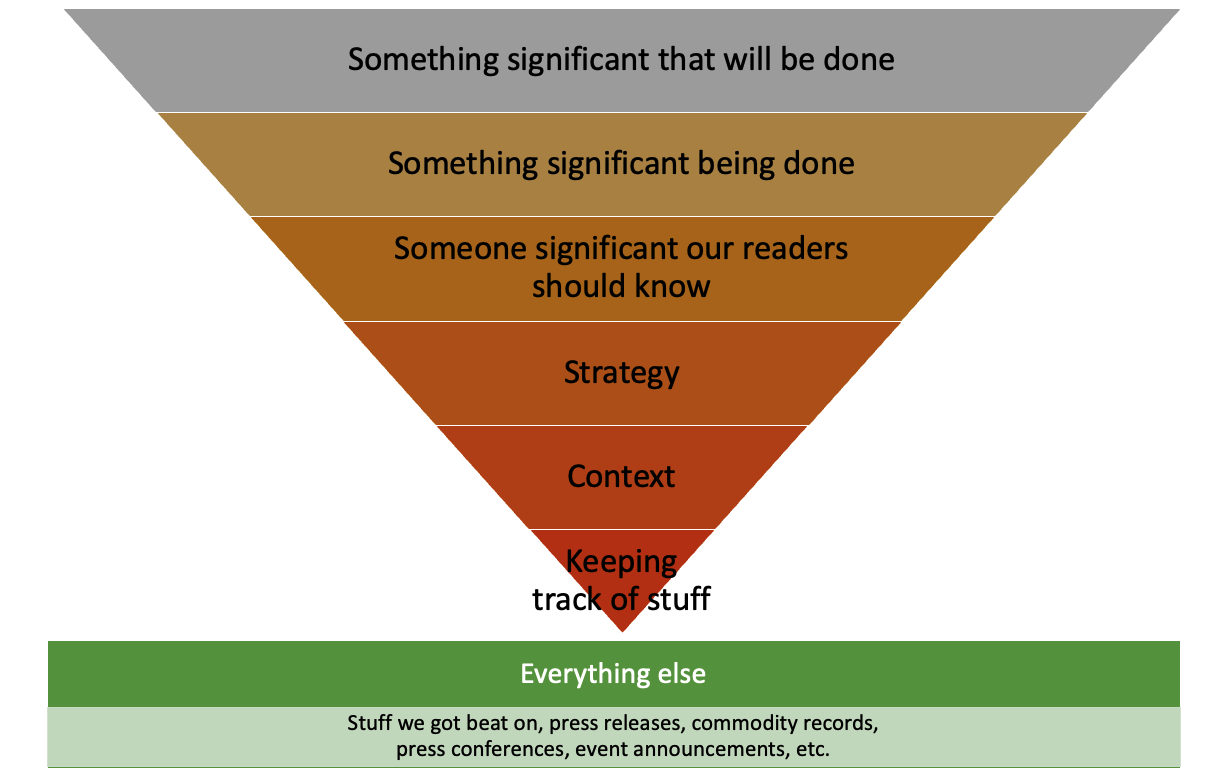
\includegraphics[width=0.8\linewidth]{images/story_hierarchy} \end{center}

\normalsize
People is a main thing: Q-and-As and profiles of significant people help you with the sourcing part of things. \enquote{Significant} is doing a lot of lifting in that sentence: If you're going to spend the time spotlighting someone, it should be someone you expect to help you get stories in the first two tiers.

Strategy and context fall into the same sort of mindset. These are stories in which you step back from the significant thing and explain how a business is planning for the next significant thing or help our readers understand where a significant thing fits in. Again, though, that only fits in in service of reporting on significant things that will be or are being done.

You should have a Q-and-A every week (we'll talk later about how to do them efficiently) as well as a strategy or context piece.

Finishing out the list of stuff is the still necessary but less important group of things that I'm calling \enquote{keeping track of stuff.} The bottom of the pyramid is the easiest bit to do --- and, as a note of warning, something that is far too easy to do too much of.

In this category I'm thinking of AAA report on gas prices, monthly roundup of vacancy rates, credit union membership figures, an update on port traffic, unemployment figures \ldots{} easy stories that may lead to other stories, but at the least keep you engaged with the industries you cover and keep the website beast fed.

You should have three to four of those sorts of stories a week.

Importantly, \emph{you should not spend a lot of time on them}. These are not the stories we got into journalism to tell; we do them because they should help lead to the more important stories.

\hypertarget{final-thoughts}{%
\section*{Final thoughts}\label{final-thoughts}}
\addcontentsline{toc}{section}{Final thoughts}

There are many different ways to judge the worth of what we do --- the reporting should be robust, the writing should be narratively engaging, etc. --- but above all, the key thing I'm looking for in a JBJ story is meaningfulness.

\leavevmode\vadjust pre{\hypertarget{storiesbox}{}}%
\begin{greybox}[frametitle=Onboarding Path]
A lot of the things in this section will play out over your first 90 days. The goal is not to have you master all of this in your first week, but I want to set out from the beginning what we're aiming to do.

\end{greybox}

There are two components that go into this.

First, it is vital to keep in mind who our audience is. We cover business. This covers a wide gamut --- retail sales to fintech to culture to real estate, and everything in between --- but this focus always has to be kept in mind. Most of the stories you do should have a dollar sign in them. Most of the people you quote should in some way be shaping the local economy.

Second, you should be looking for stories that can lead to action. A contractor decides not to work with a company because of improper behavior we've uncovered. A retailer decides to locate in a particular shopping center because of the big tenant we've told them is coming. Projects stop or start because of details we're let our readers know about.

Whether it's a quick q-and-a or an in-depth investigative piece, the goal is to write things that enable readers to change their trajectory: journalism that introduces a reader to a new business opportunity, or changes the way a reader thinks about a part of the city, or helps readers understand and make better decisions in their career, or in some other way provide new information about or a new understanding of the First Coast economy.

Every day, you should come in looking to:

\begin{itemize}
\tightlist
\item
  Break news. If you're not finding stuff out first, our reporting is less valuable to our readers.
\item
  Provide context. Our readers look to us for information they can act on. We need to tell them why events matter, what they mean and what's coming next.
\item
  Make introductions. Jacksonville is a big, spread-out city. You need to know the most important people on your beats and make sure the rest of the business community knows who they are.
\end{itemize}

The thought that should be forefront in your mind as you search for stories is \emph{why does this matter}. There's many ways to answer that question; here are some of them:

\begin{itemize}
\tightlist
\item
  How can we help our readers make money?
\item
  How can we help our readers spend money?
\item
  Who is being affected, positively or negatively, by the flows of money on the First Coast?
\item
  Who are the people winning and losing in the fight over money that our readers should know about?
\item
  Who is making money who shouldn't be, or doing so in a way that they shouldn't?
\item
  What novel things are being done with money, either strategically or operationally?
\item
  How can we help our readers avoid being scammed out of their money?
\item
  How can we make sure the money our readers have entrusted to the government is being spent wisely?
\end{itemize}

As you start out, many of the stories you do will be things that businesses hand to you, and the initial enterprise work you do will be focused on building on stories that have come before. Both of those buckets of work will continue to be part of the mix as you get acclimated, but if you take the approach laid out in this section, you'll quickly get to the point where you're the one driving the conversation.

\hypertarget{setting-a-base}{%
\chapter{Setting a Base}\label{setting-a-base}}

The next few weeks --- and the rest of this document --- are designed to get you up to speed as a new JBJ reporter

Over the coming three months, your focus will be on building up a credible network of sources, digging out stories and learning how we expect you to juggle daily coverage, evergreen pieces and enterprise reporting.

Before we get to that, though, I wanted to lay out your to-do list for the first week or so, with everything here designed to help set the base for what is to come.

\leavevmode\vadjust pre{\hypertarget{basebox}{}}%
\begin{greybox}[frametitle=Onboarding Path]
We hired you because we think you can report and write at the level we're looking for --- and that typically means that you want to jump into producing journalism. That's good \ldots{} but I've found that we get the best results when a new reporter has a little bit of time to get acclimated to what's going on.

\end{greybox}

\hypertarget{morgue-dive}{%
\section*{Morgue Dive}\label{morgue-dive}}
\addcontentsline{toc}{section}{Morgue Dive}

While I assume you want to start writing as soon as possible, my expectation is that you're starting the job knowing little about Jacksonville or what's going on here. So, step one is to get you up to speed.

First, start by reading.

Starting with the JBJ, read through what was being covered in August 2023, October 2023 and November 2023, and what was being written about in May 2024, July 2024 and July 2024.

Why these dates? The goal is to see what was being covered a year ago, with the idea that stories occur in cycles: If there was something happening around this time last year, there's a good chance that it could be something you should be looking at now.

The more recent dates give you a sense of stories in motion: As you look at those, you should be thinking of things that might need to be updated or advanced.

For the JBJ stuff, your focus should be on your beats. Do this in the CMS (making sure to open the links, not the actual stories) and use the Channel filter to narrow things down to the stories you care about

Once you're done with our archives, take a look at the Florida Times-Union, WJCT News and the Jacksonville Daily Record. While our coverage aims are not identical to those publications, there's enough overlap (and stories that they've covered that we might not have gotten to) that you'll find ideas, avenues of exploration, etc.

Then, take the Lists from the Book of Lists that pertain to your beats and start googling. See what has been written about these companies by outlets either local or national; check out their sites and LinkedIn pages and see what the company and people associated with the company are posting.

Along the way, you'll find other publications that touch on topics we care about (the Jaxon does interesting stuff touching on real estate, Trains Magazine can be a good place to see what's going on with railroads, Edible Northeast Florida provides a specific window into the local restaurant scene, etc.)

As you're doing all of this, make notes:

\begin{itemize}
\tightlist
\item
  Who are the people who pop up who you should connect with?
\item
  Who should you be following on social media? (LinkedIn across all beats, Instagram on the retail beat, but wherever you find sources works.)
\item
  What governmental agencies might have records that would be worth requesting?
\item
  Are there trade publications you should look at regularly / we should look at getting a subscription to?
\item
  What stories were big a year ago that might have fallen off the radar and should be revisited?
\item
  What happened a few months ago that might deserve a follow-up?
\item
  What stories did we miss during the interregnum before you started that we should try to get to now?
\item
  What do readers in general seem interested in?
\end{itemize}

\newpage

\leavevmode\vadjust pre{\hypertarget{morguebox}{}}%
\begin{greybox}[frametitle=Onboarding Path]
You'll spend several days doing the morgue dive, and you should treat it as an important part of the onboarding process. At the end of it, you should have a robust document with a number of people you want to connect with and a list of things that you think might be worth jumping into with your initial stories.

\end{greybox}

\hypertarget{lay-of-the-land}{%
\section*{Lay of the Land}\label{lay-of-the-land}}
\addcontentsline{toc}{section}{Lay of the Land}

Jacksonville is the largest city by land mass in the continental U.S., mainly due to the 1968 consolidation that merged the city with (and get used to hearing this) DUUUUVAL County.

The metro area stretches from the border with Georgia to the north to Flagler Beach to the south. The western boundary is a semicircle stretching through Macclenny, Keystone Heights and Palatka.

There's no way we could cover all of that or that you could find your way around that entire stretch --- but I think it's helpful to have some sense of the terrain.

(For the record: The areas in the MSA that we care most about are Duval, St.~Johns, Nassau and Clay counties, in that order. If we find news in Flagler, Putnam and Baker, we should cover them, but \emph{do not} put a lot of effort, particularly initially, in anything beyond the top four counties.)

Soon after you start, I'll take you on a tour of downtown, giving you a quick sketch of the urban core. The future of downtown and efforts to revitalize it are one of the key stories we care about, and it cuts across beats, so I want to make sure you have some sense of where things are.

On your own, you should spend an afternoon driving around Duval County, getting a sense of how the various pieces fit together. To help with that, here's a map that takes you to a bunch of different places: \url{https://maps.app.goo.gl/cS92BDfvce2xYqYa6} (The exact spots don't matter, mostly; they're just to get you in the general locale.)

We'll talk through that map so you understand why those places are there, but I'll leave it up to you to plot a route that works depending on where you're living, etc.

As you do the driving around (and make sure you keep track of mileage and expense it), take notes: What things are you seeing that seem intriguing or don't make sense or feel like they could point to a story? I \emph{do not} expect a list of valid story ideas out of this little jaunt, but I do expect you to create a list of starting point of things that might be interesting.

\hypertarget{tap-in-to-acbj}{%
\section*{Tap in to ACBJ}\label{tap-in-to-acbj}}
\addcontentsline{toc}{section}{Tap in to ACBJ}

One of the benefits of working for a company with 40-plus publications filled with people doing things similar to what you do is that you can tap into a wealth of in-house expertise.

As you are getting your feet under you, spend some time looking around ACBJ and see what your peers are doing. In many cases, the editors might have suggestions for particular reporters to follow, but it can also be valuable to simply browse some other markets and see what they're up to.

In this vein, look at the list of slack channel based on various beats. Some of these are more active than others, and the most robust ones can help direct you to stories you might not have thought of, resources you might not be aware of and other reporters who might be able to help you if you run into issues.

Through your bizjournals.com account, you can sign up for emails from any of the markets; starting out, the other Florida markets would probably be a good place to start when it comes to connecting with the company overall. (You should, of course, make sure to sign up for \emph{our} emails \ldots)

\hypertarget{next-steps}{%
\section*{Next Steps}\label{next-steps}}
\addcontentsline{toc}{section}{Next Steps}

By the end of your first week, you should have a pretty robust list of people, organizations, topics and --- hopefully --- some story ideas that will provide the base for the weeks to come.

A few days after you start, we'll start talking about the list you made and (as I go into great detail in the next section) you'll start focusing your attention on sourcing.

\hypertarget{sourcing}{%
\chapter{Sourcing}\label{sourcing}}

\hypertarget{why-sourcing-matters}{%
\section*{Why sourcing matters}\label{why-sourcing-matters}}
\addcontentsline{toc}{section}{Why sourcing matters}

What is the most important thing on the minds on the people running the companies in the industries you cover? What fears and hopes do the people interacting with those industries have? Who are the movers and shakers? How are they about to move and shake? What stories do they want told? What stories do they not want told?

How do all of those things affect the broader Jacksonville business community? How does it affect investors? How does it affect minority communities? How does it affect other industries? How does it affect those in power, those who want to be in power, those who are powerless?

What is coming that people need to be prepared for? Suppliers, shippers, brokers, builders, retailers, customers, investors, executives, residents --- what do they need to know to understand Jacksonville's economy and what's on the horizon?

\leavevmode\vadjust pre{\hypertarget{sourcingbox}{}}%
\begin{greybox}[frametitle=Onboarding Path]
This might be the most important section in this entire document. To do the journalism the JBJ aspires to, you \emph{must} be well sourced. Sourcing will be a regular part of our one-on-one conversations and should be \emph{the} main thing you do over your first weeks here.

\end{greybox}

I'm going to spend a lot of time throughout this document talking about sourcing, and the reason is all of those questions above. \emph{You can't answer them by looking at press releases. You can't answer them by talking to flaks. You can't answer them by looking at data without having a person provide context. You can't answer them while sitting in the newsroom.}

Answering those questions is our purpose, and that means you need to get out of the office and forge relationships with those who can help you understand what questions need to be asked and what the answers are.

Like any media organization, we have a decent amount of flotsam. To keep the beast fed, you're going to do some briefs (quickly; we'll talk about that later.) You're going to do some Q-and-As and cover some meetings and rewrite some press releases (again, quickly, and more later).

But the thing that got you into this business --- or at least the thing that has you working here --- is that I believe you want to break news and own stories and lead conversations. You want to be first and best a lot of the time, and at least one of those the rest of the time.

The only way you can do that is by sourcing. I'll be blunt: If you can't source, this is not the job for you. That doesn't mean you have to source in the exact same way I or other ACBJ journalists source. What it does mean is that you have to work, from the get go, at building up a source network that will let you answer the questions we started with, that will enable you to break news, explain why it matters and prepare our readers for the future.

\hypertarget{what-i-mean-by-sourcing}{%
\section*{What I mean by sourcing}\label{what-i-mean-by-sourcing}}
\addcontentsline{toc}{section}{What I mean by sourcing}

Depending on your background and experience level, you might be a little hazy on what I mean by sourcing, so let me play that out.

Business reporting presents some different challenges compared to other beats (I'm not saying it's harder, just different.) Most of what we cover is not place bound; there's not a locker room to visit or a city hall to hang out at. While we do cover some meetings, doing so is not a focus, which takes away a contact point. Finally --- and somewhat paradoxically --- forging the connections you need can be harder on a business beat because there are many people looking to give you the information \emph{they} want you to have; navigating around gatekeepers is vital.

So sourcing is not getting on the distribution list of PR people or attending board meetings or interviewing people. You should do all of those things, of course, but the goal is to go deeper.

Sourcing is developing a relationship with people who can tell you what is truly happening on the topics you care about. If someone is a source, you can reach them when they're on vacation if something big is happening. If someone is a source, they'll tell you things before the information is public --- before the press release goes out or the lawsuit is filed or the record is released.

You are well sourced when you have information that isn't being pushed out --- not necessarily secret information, but information that you have gleaned from talking to the people involved in the story. You are well sourced when people call you back at difficult times.

You are well sourced when you have an in-depth knowledge of the beat --- when you can confidently say \enquote{these are the issues that matter on the topics I cover.}

We'll talk about idea generation a bit later, but two points that matters in this context: First, after your first few weeks on the job, you should start having a list of stories you're chasing --- things that you hear are happening or will happen that you can't nail down yet.

The nailing down is both a sourcing and reporting task; for now, though, focus on the first part of that statement: You need to be connected with people enough that you know things are out there to chase. Second, and we'll discuss this when it comes to pitching stories, but your objective is to have most of your pitches start out with some variant of \enquote{ told me.} \emph{That} is the overall goal of all of this.

\hypertarget{how-to-start-developing-sources}{%
\section*{How to start developing sources}\label{how-to-start-developing-sources}}
\addcontentsline{toc}{section}{How to start developing sources}

Sourcing is building a relationship, and that relationship is going to start with you reaching out to many people in your first few weeks here.

The initial list of people you reach out to will be comprised of:

\begin{itemize}
\tightlist
\item
  a list of the first people you should reach out to, which you'll get a few days after starting
\item
  whatever names you came up with during your morgue dive --- essentially people that have been written about recently by us or others
\item
  people at the top companies on the Lists that you care about
\end{itemize}

Each day for the next few weeks, you should call (preferably), text (depending on the person) or email (if all else fails) at least three people who you want to get to know. The goal is to reach out to 50 or so people in the first month you are here.

(There is a window here: Badgering someone to meet with you in the first three months is natural: \enquote{You're an important person who I need to know to do my job; we should talk.} That pitch is harder when you've been here for six months and have never reached out.)

The goal of that initial contact is to at least get a phone conversation. Ideally, you want to schedule in-person meetings with as many people as possible --- breakfasts, lunches, coffees, drinks, drop-ins at their office, anything that gets you spending time with the person.

Let me note: This isn't easy. Getting in touch with a PR person is simple, but getting lunch with a CEO will require perseverance.

By your second month here, you should be looking to have three in-person meetings each week; by the end of your 90 days, you should have had in-person meetings with at least two dozen people and reached out to 100.

\hypertarget{sourcing-is-not-reporting}{%
\section*{Sourcing is not reporting}\label{sourcing-is-not-reporting}}
\addcontentsline{toc}{section}{Sourcing is not reporting}

During those in-person meetings (or on the phone, if that's all you can get), there's two things you're looking to accomplish:

\begin{enumerate}
\def\labelenumi{\arabic{enumi}.}
\tightlist
\item
  Start to develop a relationship. You want to come away from these meetings with the person's cell phone number and an understanding that you'll be back in touch. You need to convey that you're interested in what they do.

  \begin{itemize}
  \tightlist
  \item
    You want them to know that you care about their company and industry and want them to come to you with news.
  \item
    You want them to begin to trust you. This involves you showing an interest and knowledge of what they do.
  \end{itemize}
\item
  Begin to gain information about them, their organization and your beat in general. The questions I go into these meetings with are

  \begin{itemize}
  \tightlist
  \item
    How is your business doing? What's been some recent things of note? (Of course, you should have read up on the company beforehand if possible, and already know anything big that has happened.)
  \item
    What are they looking forward to?
  \item
    What are the major issues happening in their industry?
  \item
    What stories do they think you should be covering?
  \item
    Who else do they think you should talk to?
  \end{itemize}
\end{enumerate}

Notice that that list of information very likely does \emph{not} lead directly to a story. If in the conversation the proto-source says something that feels like it should be written about now, puruse that; I'm not saying to leave stories on the table.

What I am doing is drawing a distinction between \emph{sourcing} and \emph{interviewing}.

Most of reporting life is spent interviewing people --- getting information from people (sources and others) directly for a story. That should be part of your professional relationship with sources, but interviewing doesn't do a lot to build the relationship. One way of analogizing it: Sourcing is like inviting someone over for a cookout. You might ask them to pick up ice on the way over, but the focus of the interaction is building the relationship. Interviewing is like asking them to help you move.

If you only talk to people when you need them for a story, they're not a source.

\hypertarget{who-do-you-source-with}{%
\section*{Who do you source with}\label{who-do-you-source-with}}
\addcontentsline{toc}{section}{Who do you source with}

Everyone.

I mean this slightly tongue in cheek, but only a little. Everyone is a source: You want the CEO, you want the junior person just starting out, you want the truck driver, you want the head of the department and the worker bee and the executive. How you manage these relationships will be different depending on the person, and the job, etc., but you want people in the C-suite and people on the shop floor and everywhere in between.

\enquote{Everyone} isn't terribly helpful in thinking through sourcing, though, so let me give you two useful ways to think through who to reach out to:

\begin{enumerate}
\def\labelenumi{\arabic{enumi}.}
\tightlist
\item
  Follow the process. Pretty much everything we cover is part of a chain of events. You want sources at every link in that chain.

  \begin{itemize}
  \tightlist
  \item
    A building is being built. Who is part of that chain? There's the developer behind the project, the engineers and architects who design the structure, the lawyers who get it through the system, the construction company that builds it, the broker that leases it, the other broker that sells it, and more. You want connections at each of those points.
  \item
    An item is being imported. Who is part of that chain? There's a customer who orders it, a broker who arranges transportation, a shipping company that gets it to Jacksonville, a trucking company that brings it to a warehouse, a warehouse operator that stores it \ldots{}
  \item
    A restaurant is opening. Chef with an idea, broker who finds space, designer who shapes the space, contractor who builds it out, social media person who makes sure we know about it \ldots{}
  \end{itemize}
\item
  Think of levels. This is like the vertical version of thinking through the process.

  \begin{itemize}
  \tightlist
  \item
    The general contractor building the building has subs; the subs have employees. The contractor is probably part of a trade group.
  \item
    A restaruant group has the CEO, and the chefs at the indiviual restaurants.
  \item
    A railroad has the executives, and the division heads, and the union chefs, and the workers \ldots{}
  \end{itemize}
\end{enumerate}

As you go over your initial list of contacts and start turning them into sources, you'll start developing a schematic of the beat. Take some time and look for holes: Are there people at certain points in the chain or at certain levels that you're missing?

One note: In general, PR people are not going to be your best sources. PR people, by and large, are not sources. A CEO can be a source. A division head can be a source. A train conductor can be a source. The person paid to tell you what the company wants you to hear is not a source.

That isn't a blanket statement; there are definitely some PR people who may serve a sourcing role, and others who, while they may not be sources, are helpful people to know.

What you're looking for in a source is someone who know things that aren't out there yet and will tell you those things. I'm not saying you're going after the Pentagon Papers, but if the person is just giving you the information that they're supposed to, you don't need a relationship with them.

While talking about PR people --- I bang on about getting people's cell phones, and this is why. On a very basic level, if you can't reach them --- if you have to go through a PR person, if you can only reach them in the office --- they're not a source. If they don't answer when you call, they're not a source, either.

\hypertarget{rinse-and-repeat}{%
\section*{Rinse and repeat}\label{rinse-and-repeat}}
\addcontentsline{toc}{section}{Rinse and repeat}

OK, so you've spent your first few weeks calling/texting/emailing. You've continued doing that (at a lesser rate) in the next few weeks while adding in-person meetings to the mix.

By the end of your first 90 days, you've reached out to 100 people and met with a few dozen.

Then you have to keep the flywheel turning.

By the end of the first three months, you'll be circling back to some of those initial contacts. You'll have the people you click the most with, you'll have the people who give you the best information, you'll have the beginning of some source relationships. Now you have to build them, through texts, calls and meetings.

As you settle into your beat, the expectation is that you'll have at least two in-person sourcing meetings a week, and regular texts and phone calls. A simple metric: Call or text at least two sources every day (we can talk about strategies, but approaches will differ depending on the person), and set aside time once a week to schedule in-person meetings.

You have to immerse yourself in your beat in other ways, as well. You should be reading what your sources read (trade publications, social media accounts, etc.), looking for things that will give you an excuse to reach out. (\enquote{I saw that X is happening in Boise. You know if anything like that is going on here} or \enquote{I saw that your company got an award for safety. That's pretty cool. Figured I'd just call and say congrats.})

Gatherings are also an important part of the mix. NAIOP awards and Propeller Club holiday parties and Women's Food Alliance meetings \ldots{} going to these things will help build the relationship, will enable you to find more people and will make it easier to reach out to those people to chat.

I said earlier that interviewing isn't sourcing --- but that doesn't mean you can't use an interview as an entree point. Call up the CEO to set up time to stop by for a Q-and-A, giving you some facetime. Get their cell phone number. Call them up to see what they think about a thing. Set up lunch. Call them or text them every few weeks to touch base and to build the relationship.

You also have to make sure you don't plateau. Sure, you have one cold-storage person and one office broker and one restaurateur you have a good relationship with. You're still building your network. You should reach out to some of the people you connected with earlier and continue building your budding relationships.

Time is a vital part of the sourcing process, to be sure: By the end of your first year here, you should have a solid, robust base.

But you can't expect sources to just accrete. For many reporters, sourcing can be challenging. Half our time is spent in our own head, focused on a computer screen. Making sourcing a constant and regular part of your workday will pay off with huge dividends.

\hypertarget{keeping-track}{%
\section*{Keeping track}\label{keeping-track}}
\addcontentsline{toc}{section}{Keeping track}

One final thing: As you're going through your sourcing journey, it's important to keep track of everyone you speak with --- for your benefit and for the benefit of the rest of the staff.

To help with that, you should log your sourcing activity in \href{https://acbj-my.sharepoint.com/:x:/r/personal/tgibbons_bizjournals_com/_layouts/15/Doc.aspx?sourcedoc=\%7B7DE7F8A6-944D-4A13-8CAC-40945F1D0FF7\%7D\&file=Sourcing.xlsx\&action=default\&mobileredirect=true}{this spreadsheet}. This will allow you to look back at where you're strongly sourced and find the areas you need to shore up, will help avoid duplication of effort and will allow us to build up a stronger base for those who come after us.

\hypertarget{records}{%
\chapter{Records}\label{records}}

By and large, the way that we find stories are though people (hence the section on sourcing) and through records.

Sourcing is the most important part of that duo: If we're doing our jobs properly, people can tell us about stories before they're evident in the records, and knowledgeable people can direct us to look at records we might not otherwise review.

Our records reporting falls into a couple of different overlapping areas. As exhaustively detailed later in this document, each reporter has records related to real estate that they should look at every day. It is not uncommon for those records to be the tripwire that first alerts us to news happening.

Our reporting goes beyond that, though, with requested records and a variety of data sources playing into what we provide our readers.

In this section, I'm going to run through a brief introduction on the records we use the most, mainly to make sure you know what is out there. We'll then look at the broader categories of records that may be of interest and then wrap up by talking about how to make records-based reporting part of your overall repertoire.

\leavevmode\vadjust pre{\hypertarget{recordsbox}{}}%
\begin{greybox}[frametitle=Onboarding Path]
Records reporting (and the adjacent skill of data reporting) will take some time to learn if it's not part of what you've done regularly. As you start out here, you should focus on two things: spending time with records on a daily basis and cultivating an overall mindset to be looking for records and data that will bolster your reporting.

\end{greybox}

\hypertarget{the-basics}{%
\section*{The basics}\label{the-basics}}
\addcontentsline{toc}{section}{The basics}

There are some public record sources that we turn to on a regular basis to find details that can flesh out a wide variety of stories. You should familiarize yourself with these sites and use them often:

\begin{itemize}
\tightlist
\item
  \href{https://search.sunbiz.org/Inquiry/CorporationSearch/ByName}{Sunbiz}: The Florida Division of Corporations keeps track of every company that does work in the state (more or less). Through this site, you can find out details about the companies you're writing about: Who are their officers? When were they started? What other companies are they tied to?
\end{itemize}

This is an important backgrounding site, but some caveats do apply. One very important one: \emph{The registered agent name doesn't necessarily mean anything.} Just because two companies have the same registered agent \emph{does not} mean that they are connected. For many limited liability companies, the corporate registry will be a bit of a dead end, so don't overly get your hopes up. One tip: google the \emph{address} of the authorized person(s); this can often point you in a useful direction.

\begin{itemize}
\item
  Property appraiser for \href{https://paopropertysearch.coj.net/Basic/Search.aspx}{Duval County} and \href{https://qpublic.schneidercorp.com/Application.aspx?App=StJohnsCountyFL\&Layer=Parcels\&PageType=Search}{St.~Johns County}. This will give you information about who owns a property you care about, who owns nearby properties, when buildings were built, when sales took place, etc. If you have an address, the property appraiser is a good first step; it will give you the name of the property owner, which you can then plug into Sunbiz.
\item
  The Jacksonville \href{https://jaxepics.coj.net/}{Building Inspection Division}. We'll talk a lot about permits in the next section, with an eye toward using those records to break news. You should also turn to this site throughout the reporting process. Writing about a restaurant opening? A new warehouse? This is where you can find out how much construction cost, who built the structure and similar things.
\end{itemize}

\hypertarget{other-records}{%
\section*{Other records}\label{other-records}}
\addcontentsline{toc}{section}{Other records}

I mentioned Sunbiz earlier; while that is the most commonly use source of state records, there's a few others that often come in handy.

One of the most useful sites is the Department of Business and Professional Regulation, which has a nifty \href{http://www.myfloridalicense.com/dbpr/instant-public-records/}{instant public records} subsite.

This site is probably most used on the retail beat --- the \href{http://www.myfloridalicense.com/DBPR/alcoholic-beverages-and-tobacco/public-records/}{alcohol records} enable us to do things like examine \href{https://reportertim.github.io/breweries_data.html}{the local brewery scene} and do the weekly Roach Report. (The Roach Report data can be \href{http://www.myfloridalicense.com/DBPR/hotels-restaurants/public-records/\#1506344763000-101d4ee5-7a59}{found here}; \emph{this is something the retail reporter should do weekly.})

That said, the state also licenses harbor pilots and architects, hotels and yachts \ldots{} there are stories in that data on the most dangerous elevators and most successful engineers and more, if you want to dig them out.

Florida has a plethora of things that are public records, on both a state and a local level. While this list lays out how to access the items that have proven useful in the past, I don't assume this is complete. If you come across something that might be useful on your beat or for others, or if you find a trove of data and just think there might be potential there, please let me know.

There's also plenty of federal records.

The industrial reporter should spend some time looking at the \href{https://transtats.bts.gov/}{Bureau of Transportation Statistics}, for instance, which has a plethora of transportation data, as well as things like the \href{https://transtats.bts.gov/}{Surface Transportation Board data page}.

The real estate reporter could find stories in the \href{https://www.consumerfinance.gov/data-research/hmda/historic-data/}{CFPB's HDMA data}, and the \href{https://fred.stlouisfed.org/}{St.~Louis Fed's economic data} site could provide information that would make a retail story more robust.

Cutting across beats, \href{https://www.usaspending.gov/}{USAspending.gov} goes in depth on who is getting federal money, which could feed into a variety of stories.

And, finally, we have access to \href{https://pcl.uscourts.gov/pcl/index.jsf}{Pacer, the entry point to federal courts}. While no one is tasked with looking at that regularly, it can be a good source of stories, usually after we've been tipped off to look at something in particular.

That list, of course, is woefully incomplete, with many data sources being either beat specific or even just story specific. As you are getting your hands around your beat, be on the lookout for data repositories that might be useful: Any time you're doing a story or having a sourcing meeting and someone mentions records or data, follow up to find out where that information is from and if you can get access to it.

\hypertarget{data}{%
\section*{Data}\label{data}}
\addcontentsline{toc}{section}{Data}

In writing this section, I've somewhat conflated records and data, and I want to tease those two things apart a bit. While we don't have a dedicated data reporter on staff, we have people with varying levels of skill in Excel, R and Python --- which means that if you don't have those skills, you have somewhere to turn.

Many, many stories should have some sort of data component. That might be as complex as \enquote{how many of this thing happened in different ZIP codes over a decade} or as simple as \enquote{what is the average rent in this neighborhood today.} Any story that is focused on something changing over time or varying between areas is best told with some amount of data underpinning the narrative.

As you think through who you should talk to for a story, also think about what numbers might be available to support or flesh out what you're hearing from sources. (Or to contradict what you're hearing from sources; it is not uncommon for \enquote{the narrative} to be one thing but for the truth to be something else once you get the numbers.)

On a basic level, when a source tells you a number, ask where it came from. Oftentimes a simple story can lead to something with more depth if we go back to the original source of the data and look at the information in context.

\hypertarget{records-requests}{%
\section*{Records requests}\label{records-requests}}
\addcontentsline{toc}{section}{Records requests}

Everything laid out above dealt with records that you can look up independently. That should not be the end of your records-based reporting.

You should cultivate a mindset of regularly requesting public records from any public entity you deal with --- the city, the state, independent authorities, etc.

On a basic level, pretty much every meeting should lead to records request (most likely both before and after the meeting). As laid out in the section on covering meetings, you should be requesting agendas and supporting documentation as soon as they're available. If something newsworthy happens in the meeting, you should request whatever background information there might be.

Every bigger story you do should have you stop and consider what public documents might be available: Could someone have emailed the mayor about this? Did something need to be filed with the state? High up on the frustration chart is when you've broken a story based on sourcing, but someone else advances the news by getting records that you didn't think to ask for.

You should also have regularly reoccurring records request. We know, for instance, that the master developer of Cecil Commerce Center sends a report to the city four times a year; the industrial reporter should have a calendar reminder to ask for that. We have ongoing coverage on downtown projects; the real estate reporter should be asking for any new records related to those on a regular basis.

Making such requests a regular part of your reporting practice will set up a pipeline of documents coming in that will lead to future stories.

(To help keep everything straight, I like using a spreadsheet \href{https://acbj-my.sharepoint.com/:x:/g/personal/tgibbons_bizjournals_com/Ea65ng1GEW9OqWxEPRx1TzkBMyipS5wkbaYueyRBy6mmkw?e=NFxJmG}{like this}, which you can feel free to copy. Oh, and if you're new to Florida, here's a \href{https://acbj-my.sharepoint.com/:w:/g/personal/tgibbons_bizjournals_com/EfD3WnLQ15tHl5L4WWqUNpcBazng7XTyUZ-0wdpofYVfyQ?e=xzp1Bf}{template for public records requests}.)

\hypertarget{a-warning}{%
\section*{A warning}\label{a-warning}}
\addcontentsline{toc}{section}{A warning}

Dealing with records and data is an important part of good reporting --- but it can also be a tar pit. I point that out not to contradict anything you've just read but as a warning: If you find yourself spending a substantial amount of time wrangling records or data and it's not going anywhere, stop and talk to an editor.

We've had times where a reporter wasn't looking in the right spot for records, resulting in a far more laborious process than was needed. We've had times where someone with more Excel skill could show a struggling reporter how to do something more quickly. We've had times when everything was progressing as quickly as it could, but it was still taking too long, and the juice wasn't worth the squeeze. We've had times where an initial story could be written and then followed up on when a records request was fulfilled, but the reporter got beat while waiting.

While I urge you to think of how records and data can enhance your reporting, beware of getting stuck in a rabbit hole.

\hypertarget{final-thoughts-1}{%
\section*{Final thoughts}\label{final-thoughts-1}}
\addcontentsline{toc}{section}{Final thoughts}

So this section was designed to give you a good overview of both what is expected on your end when it comes to records and what information is available to you.

As we wrap up, I want to take a step back and talk briefly about the mindset and the approach you should have when it comes to records, records requests, data and public information in general.

I'll reiterate that sourcing is the most important part of the reporting process --- but dealing with records is a close second, helping you to keep sources honest, find stories sources don't want to talk about and have a deeper knowledge of the things you're writing about.

The goal is to have you always be thinking about what records and data can make your reporting better and then to get you in the habit of looking for and requesting that information. If you adopt that mindset, you'll have more and better things to write about and will make sure your not blindsided when news breaks.

\hypertarget{record-checking}{%
\chapter{Record Checking}\label{record-checking}}

While a specific beat focuses on the real estate industry, real estate as a concept in (forgive the pun) foundational to everything we cover at the JBJ. Accordingly, each reporter is responsible for staying on top of specific real estate records.

I talked about the importance of records generally earlier. This section is devoted to specific public documents that need to be regularly reviewed.

\leavevmode\vadjust pre{\hypertarget{recordscheckingbox}{}}%
\begin{greybox}[frametitle=Onboarding Path]
This section goes deeply into the weeds on specific things each reporter should be doing on a daily basis. We'll go over this in person --- you're not expected to pick it up immediately --- but it's important you begin engaging with this records quickly and often.

\end{greybox}

One note: The city of Jacksonville recently changed some things on the records that can be accessed online, and in 2024, we'll be rolling out a new tool that will assist with some of the record checking. In short, expect the \emph{process} of dealing with the records to potentially change in some ways --- but the mindset and habit of making record checking a daily part of your coverage will not.

To understand more about the development process it pertains to these records, these links might be helpful:

\begin{itemize}
\tightlist
\item
  \url{https://www.jacksonville.gov/departments/planning-and-development/development-services-division/site-development-plan-review.aspx}
\item
  \url{https://www.jacksonville.gov/departments/planning-and-development/building-inspection-division/commercial-permits.aspx}
\item
  \url{https://www.youtube.com/watch?v=4Vj3ynbHsVc}
\end{itemize}

\hypertarget{daily-checks}{%
\section*{Daily checks}\label{daily-checks}}
\addcontentsline{toc}{section}{Daily checks}

I mentioned \enquote{staying on top of records} above --- and doing so is a key part of everyone's job. Each reporter is tasked with checking a particular set of records on a daily basis, looking for stories both on their beats and for ones that other reporters might be interested in.

\textbf{Permits}

I'm starting out with permits because they generate the most news, and they're records that we all engage with.

Permits are applied actually fairly far along in the development process; for any large-scale projects, we should first notice that something is happening when the land is rezoned or a site plan is submitted.

In all cases, though, the application for a permit and the issuance of it is a sign that work is actually beginning. There's a plethora of stories that can come out of that fact, which is why all reporters should be looking at what's going on with permits.

As laid out below, each reporter will be looking for different things in the permit system. The starting point is the same:

Log into the system at \url{https://jaxepics.coj.net/} using \href{mailto:tgibbons@bizjournals.com}{\nolinkurl{tgibbons@bizjournals.com}}, with OUTPUT7rag.profile as the password. (This log-in info is likely to change.)

Go to the advanced search screen. Change the intake date to whenever you last searched. If you haven't searched in a while or you want to make sure you haven't missed anything, you can also skip the date field and search by status, looking for Active (In Review), Agency Review, In Review and Intake. (Note: I'm not 100\% sure on the interplay between actual intake date and when something hits the system, so this part of the process may have to be tweaked slightly.)

Here's how individual searches should take place:

\emph{Real Estate Reporter}

To find large residential projects, search Structure Type: Apartments, Condominiums, Single Family Subdivision, Townhouse and Job Cost: 5000000 to 1000000000

To find office projects, change Structure Type to Business Condo; Business, Office, Bank, Professional; and High Rise and drop the Job Cost to 1000000 to 1000000000.

To find hotels, change Structure Type to Hotel, Motel, Dormitory; and Transient, Hotel, Motel, Rooming House with a Job Cost of 1000000 to 1000000000.

The real estate reporter also compiles the weekly Crane Watch round up of the top six projects that received permits over the preceding seven days.

To get that information:

At \href{https://jaxepics.coj.net/}{jaxepics.coj.net}, click on the reports tab in the upper toolbar, and then select daily reports. Download the past seven days (Monday through Sunday, typically).

Delete the city logo and the first three rows. Select everything and unmerge cells. Select everything again and copy it into a new spreadsheet.

Once you have the entire period on one spreadsheet, sort by construction cost. Note the Permit Number of the top six items and go back to the city website to get the details. Pay attention to projects that have received multiple permits; I usually scan the top 20 or so to check for that.

\emph{Industrial Reporter}

To find industrial projects, search Structure Type: Fuel-Bulk Facility, Fuel-Service Terminal; Industrial, Factory; Marine Wharf; Other, Storage Warehouse; and Warehouse with a Job Cost of 1000000 to 1000000000.

\emph{Retail Reporter}

To find retail projects, search for Structure Type: Restaurants and Stores, Mercantile, with a job cost of 50000 to 1000000000.

In all cases, once you find permits that might be interesting, click on the little arrow box next to the permit number and go to the Specs tab, which should give you a sense of what the project is. You should also click on the Links tab and see if there are other permits associated with the filing. The Contacts tab will give you a starting point for talking to a person.

While all reporters keep on eye on permits, the rest are divided up, with the reporter who is most likely to find something useful keeping on top of them. As you look at these records, keep an eye out for things that would fall on other beats as well as things that you'll write about.

\textbf{Site plans}

Site plans review one of the earliest steps taken in the development process, with the city examining these plans for a variety of factors. For our purposes, these documents tell you a lot about what a project entails, including possible tenants, who is doing the work and more.

\emph{The real estate reporter is responsible for reviewing these filings on a daily basis.}

To see what site plans have been filed, go to \href{https://jaxcivilplan.coj.net/}{jaxcivilplan.coj.net}.

\emph{Without logging in}, change the Plan Type to \enquote{Civil Plan} and Search Type to \enquote{Status.} You Want to look for filings that are in Intake and In Agency Review.

Sort by Status Change Date and then click on the blue document icon on the right for anything that has changed since you last searched. Go to General Project Information and look at the Project Summary. If it looks like it might be something we're interested in, go to the attachments tab. Toward the bottom should be a link for current site plans; download those. (If you don't get them when they're first filed, they're hard to get in the future.)

Once you've gathered the documents you think we might be interested in, talk to an editor about what's worth a story.

You can also look at all the plans being reviewed by logging into the site (\href{mailto:tgibbons@bizjournals.com}{\nolinkurl{tgibbons@bizjournals.com}} / \href{mailto:xQ7IE3*2@1fU}{\nolinkurl{xQ7IE3*2@1fU}}).

Once you've logged in, click on Civil Plan and then click on Plan Review Dashboard (up top), opening it in a new tab. Click on the Export to Excel button and then open it and sort by Clock Start Date, newest to oldest. You can then get the CDN number for any interesting looking projects and go back to the website and review the plans

\textbf{Deeds}

Deeds show who is buying and selling property in the area, giving us a sense of who is coming to town, who is cashing out and where interest is the strongest.

\emph{The real estate reporter is responsible for reviewing these filings on a daily basis.}

Here's how to access the records:

\begin{itemize}
\tightlist
\item
  Go to \href{https://oncore.duvalclerk.com/search/Disclaimer?st=/search/SearchTypeConsideration}{the Duval County Court} and search by Consideration
\item
  Put 1000000 as lower bound and a zillion as upper bound (the upper bound doesn't matter; just put in 1 followed by a lot of zeros)
\item
  Change the date range to the past week (this will make sure you don't miss anything that got filed weirdly)
\item
  Sort by consideration
\item
  We care about deeds, mostly; mortgages are useful as supplemental information
\item
  Anything over \$10 million could be newsworthy
\item
  Click on the listing to bring up the documents
\item
  If you're lucky, there will be a parcel number; you can get info on the property appraiser site at \url{https://paopropertysearch.coj.net/Basic/Search.aspx}, searching for that number in the RE\# field. (You can locate the property at \url{https://maps.coj.net/duvalproperty/default.aspx})
\item
  If there is no parcel number, try searching the appraiser's site for the seller's name; the property appraiser lags the court system.
\item
  Take what you've found and talk to an editor; over time, you'll get a sense of what we care about.
\end{itemize}

\newpage

\textbf{St.~Johns Water Management District}

Water management requests are the first step for large scale developments that anticipate using a lot of water or having a major environmental impact - particularly large manufacturing operations.

\emph{The industrial reporter is responsible for reviewing these filings on a daily basis.}

Go to the \href{https://permitting.sjrwmd.com/ep/\#/ep}{Water Management District Permitting site}, click on the Search tab up top and then on Regulatory Search.

On the form that pops ups, select Baker, Clay, Duval, Nassau, Putnam and St.~Johns counties, change Date Type to \enquote{Received Date} and put in the last time you looked in \enquote{From Date.}

In general, we care about consumptive use permits and the various ERP categories. If you find one that looks interesting, click on the permit number and then download the Application pdf. Page 3, under proposed activities, will tell you want the project is.

If anything looks like it might be interesting, check with an editor.

\textbf{JEA}

Water availability requests are similar to the SJWMD filings: They're a sign that someone is about to do something that uses a lot of water.

\emph{The industrial reporter is responsible for reviewing these filings on a daily basis.}

To see these filings, go to JEA's (outsourced) \href{https://www.sagesgov.com/Home/Search.aspx}{filing page} and log in: \href{mailto:tgibbons@bizjournals.com}{\nolinkurl{tgibbons@bizjournals.com}} / incur7grits4integral*penance, selecting JEA as your jurisdiction.

Click on the search tab and set the submission date as \enquote{this week.} Set process to Developer Agreement, Development Meeting Request, Pre-Acceptance Letter Request and Service Availability Request. (The last one is the main one generating news.)

See what looks interesting --- we don't care about single family homes or septic systems --- and then talk to an editor.

\textbf{Zoning Applications}

The most interesting zoning applications usually involve bars, restaurants and other retail operations who need some sort of variance or other official sign off to open their operation.

\emph{The retail reporter is responsible for reviewing these filings on a daily basis.}

The easiest way to get this data is to go to \href{https://maps.coj.net/luzap/SearchZoningPublic.aspx}{the city's zoning map}. Click search and then look at those with a \enquote{filed complete} and a \enquote{pending} status (two separate searches). Sort by Submitted.

For anything new since the last time you checked, open the application and click through the various steps, which should be enough to give you a sense of what the project is. (We particularly care about anything that is looking to change to a planned-unit development or PUD.)

If anything grabs your attention, check with an editor to see if it's worth a story.

\hypertarget{restaurant-reports}{%
\section*{Restaurant Reports}\label{restaurant-reports}}
\addcontentsline{toc}{section}{Restaurant Reports}

These are not real estate records but fit thematically into this section as regularly checked records. These records are checked to see what local eateries have gotten in trouble with state inspectors; it will generally, but not always, lead to a story.

Here's how to check them:

Go to the Department of Business and Professional Regulation's \href{http://www.myfloridalicense.com/DBPR/hotels-restaurants/public-records/\#1506344763000-101d4ee5-7a59}{public records page}.

Select the current fiscal year and then click on District 5, which covers all of the First Coast. That will download a file.

Open that file in Excel and then:

\begin{itemize}
\tightlist
\item
  Filter Column C for the local counties: Baker, Clay, Duval, Flagler, Nassau, Putnam and St.~Johns.
\item
  Filter Column O for the dates since the last time you checked / the most recent week. (These lag by about a week)
\item
  Filter Column N to find \enquote{Emergency order recommended}.
\item
  Copy the license numbers from Column E.
\item
  Filter Column N again, this time for \enquote{Administrative complaint recommended} and then sort by Column S, which shows high-priority violations. Copy the license number from Column E for any establishments with more than five violations.
\end{itemize}

This should give you a short list of locations. Take that list and go to the \href{https://www.myfloridalicense.com/wl11.asp}{Licensing Portal}. Search by License Number, using the number you copied. Click on the proper establishment (double-check the name with the spreadsheet), and scroll down to the bottom where you'll see a link for recent inspections. Click on that to get a list of the inspections; you're interested in the most recent couple of inspections; it's not uncommon for the most recent inspection to be fine, because the issues were fixed --- so in that case look for the previous inspection.

These are written up as a roundup, with each violator getting about 50 to 75 words. Make sure to include the address so readers know precisely what place we're talking about. If a restaurant was temporarily closed, note when it reopened.

\hypertarget{public-agencies}{%
\section*{Public agencies}\label{public-agencies}}
\addcontentsline{toc}{section}{Public agencies}

We'll discuss covering meetings in a later section, but one point concerning records belongs in this section.:

\emph{You must get the agenda \emph{and the agenda package} for every public entity you cover as early as possible}.

The point of looking at these is as a tripwire: With Jacksonville's consolidated city/independent authority setup, a lot of economic activity touches on public entities at some point - usually a fairly early point - in the process, and seeing what's happening on that front is one way to keep ahead of stories.

The industrial and development reporter should be looking at the Mayor Budget Review Committee agenda every two weeks as well as the agendas for the various transportation-related authorities. The real estate and growth reporter should be keeping tabs on the Downtown Investment Authority and Downtown Design Review Board. The retail and small business reporter should be paying attention to the Land use and Zoning Committee.

Many of these meetings will not be covered; sitting through a bunch of government jawboning is often not a good use of your time. Finding out in advance what will be covered, though, is vitally important.

Get familiar with the calendar of the bodies you're responsible for, get on their mailing list and make sure you're getting all pre-meeting documents that you can as early as you can.

\hypertarget{final-thoughts-2}{%
\section*{Final thoughts}\label{final-thoughts-2}}
\addcontentsline{toc}{section}{Final thoughts}

Dealing with all of these records seems complicated \ldots{} and it will be, at first. After a few weeks of engaging with these records, it will become second nature.

Two key things to keep in mind: You need to look at these things every day; the process becomes more complicated (or impossible) if you fall behind.

Also, notice how often \enquote{check with an editor} shows up in the information above. You're \emph{not} expected to know precisely what we care about during your early days here. Talking through what you find in the documents will help focus your news judgement and make the entire process less scary.

\hypertarget{planning-production}{%
\chapter{Planning \& Production}\label{planning-production}}

So we've gone through many key steps in getting your feet under you at the JBJ, from getting to know your beat to building up a source network to understanding what we're looking for in stories.

In this section, I want to get very practical and talk about day-to-day reporting and writing, going over meetings, productivity and process things.

\leavevmode\vadjust pre{\hypertarget{planningbox}{}}%
\begin{greybox}[frametitle=Onboarding Path]
Two key points: 1. We expect a fairly high level of production at the JBJ, but it's a managable workload is you approach it properly. Read this section carefully so you know what to expect. 2. Most reporters aren't great at planning. Sharpening that skill will help immensely.

\end{greybox}

\hypertarget{production}{%
\section*{Production}\label{production}}
\addcontentsline{toc}{section}{Production}

As mentioned earlier, you're expected to have something on the order of eight to 10 posts a week. \enquote{Posts} is chosen specifically in that sentence: Not everything you file is created equally; doing eight briefs a week doesn't fulfill the mandate, but nor should you be running yourself ragged to turn around a half-dozen in-depth stories each week.

In general, you should have three full stories --- planned-out, conversation-driving stories --- each week.

The goal of these stories is to break news --- to tell readers something significant that will be done or is being done that has not been reported by anyone before. This will not always be possible, particularly in your first six months --- but that is the goal.

These stories can also fulfill our goal of providing context and strategic knowledge to our readers --- helping them understand trends that are shaping the Jacksonville economy, providing insight into how a person or company did something, that sort of thing.

The thought that should be forefront in your mind as you search for stories is why does this matter. You need to have a goal in mind with every story you tell.

These news-breaking, somewhat-in-depth stories will be 450 to 550 words; rarely would you ever go over 650 words, and only after a conversation with an editor. The expectation is that writing these stories should take about two hours. You should endeavor to get decent art with these.

You should have one story each week introducing our readers to someone they need to know. These can be profiles or Q-and-A's and should run 450 to 700 words. Profiles should take up to two hours to write; Q-and-A's should take an hour. (We'll talk more about Q-and-As in a bit). For each of these, you need a headshot of the subject, or an environmental sort of shot.

You should have two or three meeting stories/earnings briefs/reports/previews and other such stories that keep you engaged with your beat and give our readers context for the news we break. These should take up to an hour and a half to write.

You should have two to five quick-turn briefs. The number, cadence and source of these will change per beat: The reporter who covers real estate will have permit briefs, the retail reporter should be mining social media posts for quick turn stories and the industrial reporter should be monitoring state contract announcements. These are easy stories that keep our readers engaged, point to opportunities and show that we're the publication to turn to for news. These should take half an hour or so to write.

These briefs should be things where you have value to add: You're immersed in the story so you can do it quicker or with more nuance or detail, you're using it to connect with a source, you got the announcement before it went wide, something like that. If it is something more generic that anyone can cover, pass it on to an editor: You might end up doing it depending on what other people are working on, but reporters should be focused on higher-value work and the editors can do more commodity news if a story is required at all.

One note on briefs: Don't hold them. If they're assigned, the assumption is that they'll be turned in roughly immediately. There's no point, generally speaking, in scheduling a brief for later. If you don't have time to do them ASAP, let an editor know, and they can either help you prioritize or figure out a different path to take.

You should plan on having one cover story every four to five weeks. The cover story process should follow the \href{https://docs.google.com/spreadsheets/d/1NA5khaUA2TEatah0DSByH2hUVMbGpzMzeFEqfeBC0-Q/edit\#gid=1493329012}{timeline laid out here}. In general, you should have a firm pitch nailed down five weeks or more before the story is due.

Reporting out the CP should take 8 to 15 hours spread out over the course of the month. You will be given a block of uninterrupted time to write the CP, which should take around four to six hours.

The expectations is that you will always be working on a planned-out centerpiece and will also be looking for daily stories that could be elevated to be a cover story.

\hypertarget{planning}{%
\section*{Planning}\label{planning}}
\addcontentsline{toc}{section}{Planning}

Our rhythm should always be governed by the news; even as business reporters, we're going to have days that stretch beyond business hours. Days like that should happen because the news requires it, though, not through lack of planing.

Even though we should be able to jump on a big story and win the coverage wars doesn't mean that there's any value in treating every day like we're just waiting for things to unfold. To that end, we have a couple of meetings and a budgeting tool that you should use to help stay on track.

First, the meetings:

\begin{itemize}
\tightlist
\item
  Every morning, we meet at 9:30 a.m. either in person or on Teams. You'll get an invite to this meeting soon after starting. The idea is that you will, by that meeting, have a firm grasp on what your day will look like: What interviews you have, what stories are coming in, what work you're doing on future stories.
\item
  Tuesday afternoons, we have a look-ahead meeting. The first part of this gathering is focused on centerpiece stories; you should come prepared with an update on whatever CPs you have in the works. The second part of that meeting is more open-ended, giving us an opportunity to step back from the hustle and bustle to see if there is anything on the horizon we should be prepared for. This is a good time to talk about potential story ideas, things you're hearing and events coming up that might be worth covering.
\end{itemize}

Day-to-day coverage is governed by the budget \href{https://acbj-my.sharepoint.com/personal/tgibbons_bizjournals_com/Lists/JBJ\%20Planning\%203}{that you can access here}. You add things to the budget by clicking the \enquote{add new items} button in the top left corner.

In general, you should have about five to seven things on the budget for the coming two weeks --- two or three of your planned stories, the profile/q-and-a, meetings and reports, earnings, etc.

Quick-turn briefs should be discussed in the morning meeting or as they come up and then be added to the budget.

Items on the budget over the next two days (i.e., when I look at the budget Tuesday night, the things slated for Wednesday and Thursday) should be firm; unless something truly unexpected happens, they should be turned in on the day and at the time indicated.

Out days are softer; things more than a week out are basically notional --- meaning there's nothing wrong with putting a story on the budget two weeks out even if you're not certain that it will come in then. By the time \enquote{two weeks out} becomes \enquote{two days out,} though, it's on you to make sure that what is on the budget is accurate.

You can move stuff on the out days, but if you're shifting things that are scheduled for the next few days, let an editor know, since that starts affecting production scheduling.

\emph{It is your responsibility to budget stories, and to make sure the budget is accurate}. If something has been sitting on the budget for a few days, it shouldn't change at the last moment.

\hypertarget{the-budget-tool}{%
\section*{The budget tool}\label{the-budget-tool}}
\addcontentsline{toc}{section}{The budget tool}

We'll go over budgeting during one of our initial conversations, but I'll put some of the details here as well.

The most important fields that you will fill out \href{https://acbj-my.sharepoint.com/personal/tgibbons_bizjournals_com/Lists/JBJ\%20Planning\%203?viewid=a1fb1466-c5cc-4f2e-b860-514cf8dbd979\&env=WebViewList}{when you budget a story} is the headline and gist of the story. \emph{These can change} as you go through the reporting and writing process, but it is vital that you know where you're going with a story before you embark on it.

\scriptsize

\begin{center}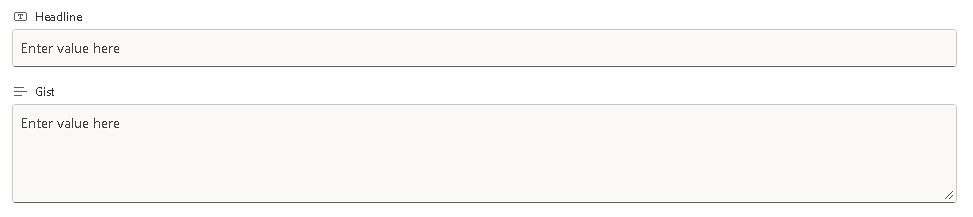
\includegraphics[width=0.8\linewidth]{images/headline-gist-new} \end{center}

\normalsize

The headline should be something that you think will grab readers' attention, and the gist should, basically, be what you think the nutgraf will be. Accordingly, this \emph{won't} be something like \enquote{Q-and-A with Sally Smith} or \enquote{DIA meeting,} but rather what you plan on getting out of those events.

\scriptsize

\begin{center}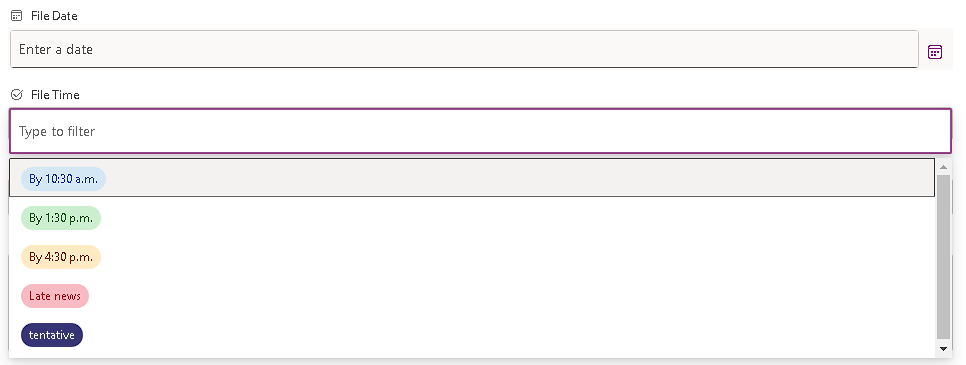
\includegraphics[width=0.8\linewidth]{images/file-date-time-new} \end{center}

\normalsize

The filing data and time are used to help us figure out what will be running when. As noted above, these are aspirational for out days and should be solid over the next day or two. If you mark a story as tentative (if, for example, you need one more interview and you think the subject might flake), let an editor know when it becomes solid.

The time field is so we don't plan a story for Afternoon Edition when it's coming in at, say, 3 p.m. and it's not a story we have to rush on. \emph{These are the latest times a story should be filed}, and represents a commitment that you'll get it in by that time. If you're not going to be able to hit the filing deadline, talk to an editor in advance. Also, don't push stuff later if there's no reason to: If a story can be sent in at 10 a.m., do that, don't wait until later in the day, even if that's the deadline.

As you're planning, think through what your day looks like. If you're doing a Q-and-A at 2 p.m. and there's not vital news in it, don't budget it to run in afternoon edition. You can still write it and file it, but there's no value in treating non-breaking-news like an emergency; there's a lot of things we want you to turn around quickly, but acting like everything is a quick-turn story is a path to burnout.

One final note on the budget tool: It's designed to help you with your planning as well as govern the production schedule. If you mark a story as \enquote{Planning,} it will not show up in the other views; no editor will be expecting it. This allows you to schedule things for the future even when they're tentative, giving you a grasp on what you have in the works.

\scriptsize

\begin{center}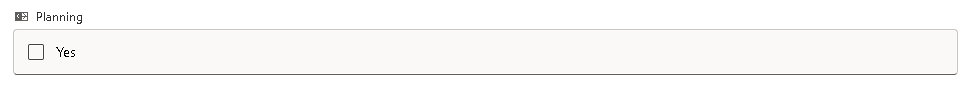
\includegraphics[width=0.8\linewidth]{images/planning-new} \end{center}

\normalsize

When we go over the tool during our initial conversations, we'll talk about the other views available to you that can help you with planning out your coverage and organizing your days.

\leavevmode\vadjust pre{\hypertarget{planningboxs}{}}%
\begin{greybox}[frametitle=Onboarding Path]
We'll go over the budget during onboarding, which should help make all of this clear.

\end{greybox}

Last thing on planning: We don't have an end of the day meeting, but please check in with me before you clock out for the day. This is a mixture of good practice and my own pet peeve, to be clear --- but it drives me nuts when reporters just vanish into the ether. A quick slack or popping your head into my office just to let me know where things stand, what the next day looks like, see if there's any unresolved issues is all you need to do.

\hypertarget{getting-overwhelmed}{%
\section*{Getting overwhelmed}\label{getting-overwhelmed}}
\addcontentsline{toc}{section}{Getting overwhelmed}

One final note that fits into this section: We tend to keep a lot of balls in the air, and I'll never be shy about asking if you have the capacity to add something else to your plate. When I ask that, I'm \emph{asking} that. Particularly with a hybrid work environment, it's easy for me to not have a truly firm grasp on everything you have going on.

If I need you to shift your attention to something, and you don't have the bandwidth to do so, \emph{let me know}: Putting something on your plate will sometimes mean I have to take something off. I'm happy to make that decision, but you'll have to let me know where things stand so I can effectively prioritize.

Along those lines: I'd implore you not to write on deadline when you don't have to.

Your focus should be on being the first with news, and often this will require fast writing and last-minute editing. \emph{But there's no reason to do that when a story doesn't require it.} If you're doing a Q-and-A interview Monday morning, plan to file it Monday afternoon --- maybe even Tuesday morning. If you have a story with multiple interviews, write as you're going along.

If you can, come into work with the reporting done on a piece and start your day by getting a post filed early, it makes everything run more smoothly while cutting down on your stress level.

\hypertarget{filing-stories}{%
\chapter{Filing Stories}\label{filing-stories}}

This is simply a quick overview of the actual process of filing a story. Some of it will make more sense once you start engaging with the CMS, but I think it's helpful to have everything you need to know in one spot.

\hypertarget{the-cms}{%
\section*{The CMS}\label{the-cms}}
\addcontentsline{toc}{section}{The CMS}

Everything you file will be through \href{https://cms.bizj.us/}{the CMS} \ldots{} although I'd recommend not \emph{writing} in the CMS: Although there is now a backup feature that might save you if things go wrong, I feel more comfortable writing in Word/Google Docs/your favorite text editor.

When you put a story in the system, there's a few other steps you have to take care of:

\begin{enumerate}
\def\labelenumi{\arabic{enumi}.}
\tightlist
\item
  Fill in all the headline fields

  \begin{enumerate}
  \def\labelenumii{\arabic{enumii}.}
  \tightlist
  \item
    News headline is your old-fashioned print headline: Tell the reader the story. (I.e, \enquote{CSX makes major acquisition})
  \item
    Email headline is a veiled headline. (I.e., \enquote{Jacksonville's oldest Fortune 500 company is about to get bigger})
  \item
    Search headline is even more explicit than the news headline. (I.e., \enquote{CSX Corp.~buys XYZ Corp.})
  \end{enumerate}
\item
  Slug will fill in automatically; if it doesn't, put in \emph{a few} words with dashes-between-them that describe the story.
\item
  For print headline, use the news headline.
\item
  The tease should also be veiled. Think \enquote{what would make a reader click through to read the story?}
\item
  Path should be automatic (/jacksonville/news); if it needs to change, an editor will do that.
\item
  Primary channel/secondary channel/topic: Every story should have one or two channels; most of these will be obvious. Don't pick a whole slew of channels; default is just primary, but add a secondary if needed. For topics, see if something fits; if not, leave it blank.
\item
  Most of the time, special categories will be blank. The exception: Anything to do with construction. If you have a story about someone building something (an office, a store, a warehouse), mark it as \enquote{Crane Watch All Markets.}
\item
  Social tease can be the same as the general tease, but if you have something that you think would play well on social media, put it here.
\end{enumerate}

Every story needs to have a photo with it. Click \enquote{find in media library} and look around to see if we have anything that seems to fit; if not, just let an editor know and we'll get some stock art.

On that note: Every time you talk to someone, ask about photos: pictures of the CEO, photos from a groundbreaking, renderings, etc. \ldots{} it's all likely to come in handy.

Related content is the only other field you have to pay attention to. Click the add button and attach five stories that seem like things that people reading your story would be interested in. They can be either be directly related or tied together thematically.

\newpage

\hypertarget{other-things}{%
\section*{Other things}\label{other-things}}
\addcontentsline{toc}{section}{Other things}

When you're done with the story, click the down arrow next to the big blue \enquote{save} button and send it to the \emph{edit desk} \ldots{} and then click over to the edit desk and make sure it's there. (The system hangs up sometimes.)

\scriptsize

\begin{center}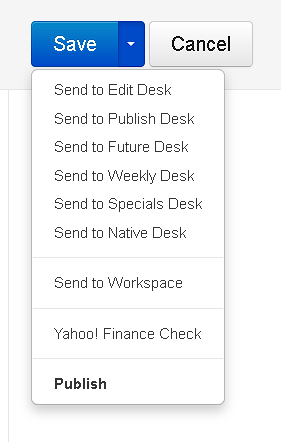
\includegraphics[width=0.6\linewidth]{images/send-to-edit} \end{center}

\normalsize

Stories should be filed as they are done. On the budget, we list 10:30 a.m., 1:30 a.m. and 4:30 a.m. as filing times; those are deadlines for the afternoon and morning email \ldots{} but there's no reason we can't post a story at 9 a.m. if it's ready then, and there's definitely no reason to file a story later in the day if you can file it earlier.

In general, you should plan to file your last story of the day earlier if there is an expectation that more work than usual might need to take place during the editing process. (Late-breaking stories obviously will come in later.) Keep in mind that your story has to be edited after it is filed, and you're expected to stick around for questions in case there are any --- so don't file a story, particularly one that is running in Morning Edition, and then jet.

When you file, let the editors know --- a post in the general newsroom slack works well --- and then be prepared for questions. If you file later in the day, be aware that you might have to wait around a bit for the story to be edited.

\hypertarget{accuracy}{%
\chapter{Accuracy}\label{accuracy}}

When it comes to writing, getting things right is \emph{the} essential part of your job.

Mistakes kill your credibility as a reporter, damage our reputation as a publication and make the job of reporting harder.

You know all of that; we wouldn't have hired you if we thought you had an issue with accuracy. That said, mistakes can happen, so I want to talk a bit about how to deal with them when they do and explore some ways that we make sure they don't.

\hypertarget{when-mistakes-happen}{%
\section*{When mistakes happen}\label{when-mistakes-happen}}
\addcontentsline{toc}{section}{When mistakes happen}

Like everything else in this document, we'll discuss all of this during the onboarding process, but I want to put this in writing to make sure we're on the same page: If there is anything that has to be changed in a story, \emph{you must talk to an editor}.

A benign typo, a source who wants you to change \enquote{around 150 seats in the restaurant} to \enquote{the restaurant will have 147 seats}, adding in the architect of a project that you didn't have when the story first ran --- any change at all requires you talking to an editor. For the minor stuff, you'll probably be told to make the change and republish, but do not do so on your own.

That conversation should not be an antagonistic one; we may need to have a deeper conversation about accuracy, but at this point, the goal is just to make sure the story is correct and up to date.

You must act quickly in dealing with requests for changes. This means responding to the source to tell them you're dealing with it and then calling an editor --- Tim first, and then James and then Stuart --- not just sending an email and waiting for them to see it.

For anything more serious, the same process applies, but the urgency is ramped up. If anyone calls about a substantial correction, here's how you should handle it:

\begin{itemize}
\tightlist
\item
  Be polite. This is not the time to argue with the source. Listen to them and make sure you understand the issue they're calling about, and then tell them an editor will get back to them shortly.
\item
  Do not argue. I know I just said that, but I want to repeat it. Dealing with an angry source is not in your job description. Pass it on up the chain.
\item
  Don't apologize. While you shouldn't argue with the source, it's also important to not swing the other way: Don't say things like \enquote{oh, crap, I did get that wrong} or \enquote{you're right, that is a mistake.} Your job at this point is not to mollify the person; it's to ascertain the situation and get an editor to deal with it as soon as possible.
\item
  Get in touch with an editor. Call, slack, email, text --- if someone says we have something substantially wrong, you need to escalate immediately and get an editor involved. (If no one is responding, you can move up to the publisher and the editorial team in corporate; we'll talk about how to do that when we discuss this, but that hasn't yet had to happen.)
\end{itemize}

\hypertarget{having-mistakes-not-happen}{%
\section*{Having mistakes not happen}\label{having-mistakes-not-happen}}
\addcontentsline{toc}{section}{Having mistakes not happen}

I started out talking about how to deal with requests for changes because following those steps is vitally important \ldots{} but even better is never having to have those conversations.

Getting to that point means making a final fact check a part of your reporting process --- but it's not enough to just read over a story and say, \enquote{well, I think it looks good.} Here's the process you should follow with every story you file; for most daily pieces, it'll take about 15 minutes.

Importantly, this process is designed to have you spend a few minutes looking at the totality of the story: While it makes sure the basics are correct, it's also an opportunity to look at bigger things, giving a final check to the facts, the overall point of the story, the way it is structured and how it is written.

Here's the steps you should take:

\begin{itemize}
\tightlist
\item
  Are names and titles correct? Don't rely on your notes; Google names, look at LinkedIn for titles. When you're sure, put \enquote{CQ} next to them in notes mode.
\item
  Are numbers correct? Again, it's good to have a source other than your notes if possible. CQ these as well.
\item
  Do you have any doubts about the overall thrust of the story or any specific details? Would you be comfortable saying everything in the story to the sources you talked to?
\item
  Have you constructed a headline and teases that are accurate and will grab readers?
\item
  Have you filled out all the fields in the CMS, including attaching a photo?
\item
  Have you linked back to previous coverage?
\item
  Does the lede do its job of hooking the reader? Can you make it shorter or grabbier?
\item
  Is the gist of the story clearly stated in the lede and/or nut graf? Does it carry through the story? Can you make it better or clearer?
\item
  Is anything missing from the story? Are there questions you still have? (If so, note those in the story and talk to an editor.)
\item
  Does the story flow the way it should - inverted pyramid, chronological, chunked, etc. \ldots{} will readers be able to follow the narrative logic?
\item
  Is there nuance you should add? Better descriptions, better quotes, additional context \ldots{}
\item
  Do you have things in the story that don't matter --- extraneous things you can get rid of? If so, cut them.
\item
  Did you use active verbs? Can you punch them up?
\item
  Is there something that happens next, and, if so, did you let readers know about that?
\end{itemize}

That list is based on on one I had hanging over my computer for most of my reporting career, starting after I made some mistakes and wanted to make sure it didn't happen again. It carried me through daily reporting, investigative work, long-form enterprise pieces and more.

If you make a checklist like that part of your daily practice, it will help you avoid corrections and should also elevate your writing in general.

\hypertarget{pitching-stories}{%
\chapter{Pitching Stories}\label{pitching-stories}}

So at this point you should have a good handle on what we're trying to do here, understand how that goal plays out on a daily basis and grasp how important sourcing is to all of this.

You've read a bunch of old stories, you've followed a bunch of people on social media, you've signed up for trade pub newsletters, you've had sources tell you stuff that matters. And, over your first few weeks, you've done assigned stories, from briefs to meetings to update pieces.

Now you want to write your own stuff.

One last hurdle: Every story at the JBJ, from a brief to a centerpiece, has to be pitched (or assigned \ldots{} but the goal is mostly pitched.)

That raises the question that many new reporters have stumbled on: How do we want you to pitch a story?

The answer is that you need two to have two things: a concrete understanding of what the story is and an explanation as to why the story matters.

Both of those statements need to be unpacked

\hypertarget{know-what-the-story-is}{%
\section*{Know what the story is}\label{know-what-the-story-is}}
\addcontentsline{toc}{section}{Know what the story is}

For the first one: If you're going to pitch a story, you need to know what it is. That may sound obvious, but if you're scrambling for a story (and God knows I've been there), it's easy to toss out a thing without really understanding it.

There are many, many things that are not stories that reporters may try to pitch as stories. A thing happening is not a story. An interesting person is not a story. A topic is not a story. A thing you heard about and would like to look into is not a story.

\leavevmode\vadjust pre{\hypertarget{pitchingbox}{}}%
\begin{greybox}[frametitle=Onboarding Path]
They key part of all of this is to take the early sections about what makes a story a JBJ story and keep it in the front of your mind as you look for things to write about: If you can't explain why something matters, you probably don't have a story. If you think there is a story there but can't articulate it, see if an editor can help you find the meaning.

\end{greybox}

They might all lead to stories --- and you might be able to fashion them into pitchable stories ---~but the bare fact of things existing is not enough.

A meeting is happening, someone was hired, someone wants to do something, the reporter says. Not enough. In that case, you need to go a bit deeper: what is actually happening; what is the thing that is or may be newsworthy.

This is a common sticking point for new reporters. \enquote{I'm going to go to a press conference.} \enquote{I'm going to cover a meeting.} \enquote{Company X has an announcement.} \enquote{A new report was released.}

That's not a story. You need to go deeper: What's happening at the press conference, what grabbed you on the meeting agenda, can you get the announcement under embargo, what's newsworthy in the report?

In this same category of things that are not stories is topics. We'll talk more about that in the next section --- when we talk about turning topics into story ideas --- but I'll mention here that saying something along the lines of \enquote{The Eastside has a lot of interesting stuff going on} could be the start of a conversation, but isn't itself a pitch.

Those are my questions at the first gate.

Many pitches fail at the second gate --- explaining why the story matters.

\hypertarget{know-why-anyone-would-care}{%
\section*{Know why anyone would care}\label{know-why-anyone-would-care}}
\addcontentsline{toc}{section}{Know why anyone would care}

Knowing why we're digging out information to put in front of our readers is vital to the reporting and writing process because it will shape what information you have to gather and how you present it.

I'll ask the \enquote{why the hell would anyone care} question in different ways --- Why does this matter? What's the impact? What can someone do with this information? How does this change things? What does this lead to? --- but the all amount to explaining why this is something readers need to know.

Let me go through some examples to make this clear.

\emph{The DIA is having a meeting.} Not a story. The reporter hasn't done the legwork to actually find out what the story is.

\emph{The DIA is going to consider changing its incentive policy at its next meeting.} This is a good first sentence. You've explained what the story actually is; I can picture a \enquote{DIA changes incentive policy} headline.

\emph{At its next meeting, the DIA is going to consider changing its incentive policy, which could change what type of businesses locate downtown.} That's a full pitch. Now I understand what story you're looking to get and who the readers of that piece could be.

Let me pause on that example for a moment because it illustrates an important point to all of this: If we're busy, and you toss \enquote{The DIA might change its incentive policy at its next meeting; should I cover it?} at me, I might just say \enquote{yes} and move on \emph{because in my head, I'm filling in the reason why it matters}. The problem with that is that you have no way of knowing that that is why I'm interested in the story \ldots{} which makes things tougher in the writing and editing process.

Having the \enquote{why it mattes} bit explicitly laid out should help writing and editing go more smoothly.

Another example:

\emph{More cargo is coming to Jacksonville from South America than Asia.} I will be sure to note that for trivia night, but I'm not sure what else to do with that information. It works as a first sentence, but doesn't answer the second.

What would a better pitch look like?

\emph{More cargo is coming to Jacksonville from South America than Asia, and now local companies are struggling to find Spanish-speaking cargo brokers.}

or

\emph{More cargo is coming to Jacksonville from South America than Asia, and I've talked to two companies that have seen business surge because of it.}

Now you're telling readers who is winning and losing, which is always a good read; you're giving readers an understanding of what they can do better; you're opening up a new way of looking at the world for readers who hadn't thought about these options before.

What's the difference between the first example and the last examples? An explanation of why someone should care.

Why would someone read this and take an action, why would they decide they need to pay to read it, why would they read it and forward it to a coworker or put it on social media, how will it affect their lives, how does it have an impact beyond the time it takes the reader to close the tab?

\hypertarget{final-thoughts-3}{%
\section*{Final thoughts}\label{final-thoughts-3}}
\addcontentsline{toc}{section}{Final thoughts}

As we'll get to when we talk about enterprise reporting, having a well-thought-out pitch is vital for any sort of longer-form writing. If we're asking readers to spend 20 minutes with a story, we need to damn well make sure it's worth their while.

But thinking this way applies even to briefs. If we're spending any time at all writing something, we need to have a good reason for expecting readers to care about it.

We're not here to tell people vaguely interesting news or serve as the paper of record or to cover something because it gets you out of the office for the morning. We're here to tell people news that they can do something with, news that matters.

Some of it will be big news, stories that we spend a lot of time on, stories that require expensive public records and deep sourcing and lots of writing time.

Some of it will be briefs that, yes, are just rewritten press releases --- but they're rewritten because there's a reason people need to know that this promotion happened, that it matters that company X bought company Y.

Some final thoughts:

First, it's important to keep in mind that everything you just read applies to \textbf{actually pitching} stories. As in, \enquote{I'm going to write a story on \ldots{}} or \enquote{I'd like to cover \ldots{}} .

None of this is to say that you can't check in with an editor to see if something is worth covering. You're new here; I don't expect you to know what we consider important. Do not hesitate to ask if we care about a particular press release or if it's worth finding out more about a development a source told you about or seeing if a broad topic would be news we would cover.

You \emph{should} be having those conversations with the editors. You are new and don't know what we care about.
Ask those questions, but ask them so you understand the lay of the land, rather than arguing for them as things you want to cover.

Those conversations will strengthen your ability to deal with the first sentence.

Second, and related, your ability to answer the second question should grow as you develop your source network. The only way to know why someone would care about the story you're pitching is to be talking to the people who care.

Finally, feel free to pitch stories, even if you're not sure we want them. I hired you because I think your viewpoint will add value to the team. If you think something is important, I want to hear about it --- if we say no, we'll explain why.

\hypertarget{covering-meetings-speeches-and-press-conferences}{%
\chapter{Covering Meetings, Speeches and Press Conferences}\label{covering-meetings-speeches-and-press-conferences}}

The focus of reporting at the JBJ is digging out information from our sources and, secondarily, from records.

That said, we do cover a decent amount of meetings, speeches and press conferences ---~if for no other reasons than doing so helps make sure we stay on top of the topics we cover and because they should be easy stories to produce.

\emph{That} said, most reporters cover these things wrong. They write boring stories and take too long to write them. They don't take advantage of the reporting opportunities presented by such events. They think they've accomplished something by sitting through four hours of bullshit and turning that into 500 words of bullshit \ldots{} which is not the reason any of us got into this business.

So how do you cover meetings, et al, properly? Let's go through the steps.

One note: I use \enquote{meetings} as a catchall for the next bit, because I got tired of typing meetings, speeches and press conferences. Most of what I have to say applies to all three; I'll pull out some specific stuff toward the end.

\hypertarget{preparing-for-meetings}{%
\section*{Preparing for meetings}\label{preparing-for-meetings}}
\addcontentsline{toc}{section}{Preparing for meetings}

If you're going to cover a meeting, a speech or a press conference you should almost always do a preview.

For meetings, this means getting the agenda ahead of time and seeing what might be interesting. For speeches and panels, you should try to get the key person on the phone for an interview beforehand. For press conferences, you should try to get the news on an embargoed basis.

This will help make sure you're fully aware of what is expected to take place at the event, and should make writing the follow-up story easier; the \enquote{after} story might simply be topping off and adding quotes to the \enquote{before} story.

All of that assumes that there is something interesting going on at the meeting. If not, you still might want to attend --- for background purposes, for sourcing, etc. --- but you should go into the meeting knowing that.

\hypertarget{writing-the-story}{%
\section*{Writing the story}\label{writing-the-story}}
\addcontentsline{toc}{section}{Writing the story}

You should never assume that a meeting in itself is worth a story. (As in, don't put \enquote{XYZ meeting} on your budget as a story.) Meetings aren't news; what happens at them may be.

Meetings, speeches and panels are boxes that (may) contain news. Far too many reporters focus on the box and not what is inside.

Too often, it's easy to treat meetings as \emph{events}, as things that are being covered. Occasionally they are, but most of the time, you should approach them as though someone else is doing an extended interview and you're pulling the news out of it.

I find my coverage radically changed when I had that realization. You're not watching a thing happen and writing about it; you're writing about a thing and the meeting or press conference is given you material for your story.

The fact that a meeting happened, even the fact that a vote was taken -- that's not the news. The news is what that vote means or, in the case of a speech, what the audience can do with whatever was talked about.

To give an example:

\begin{quote}
The City Council voted 17-2 to raise the fees charged by the city on commercial water connections.
\end{quote}

is a \emph{process} story. There's not thing in there that matters to readers.

\begin{quote}
Each new building in Duval County will be hit with a higher charge for water connections, with the change going in effect in June.
\end{quote}

\begin{quote}
The new fee comes after a 17-2 vote by City Council on Wednesday.
\end{quote}

is a story about a newsworthy thing, with the process just a component of the story.

For the press conference version of this point, you don't want to do

\begin{quote}
The Jacksonville Historical Society unveiled a plan for a museum of local music at a press conference at the site on Tuesday.
\end{quote}

rather, I'd prefer

\begin{quote}
Jacksonville has a long history with Southern rock, blues and other musical genres --- but that past is rarely celebrated.

That may soon change.

The Jacksonville Historical Society is planning a museum of local music, unveiling plans for the facility on Tuesday.
\end{quote}

\hypertarget{covering-the-event}{%
\section*{Covering the event}\label{covering-the-event}}
\addcontentsline{toc}{section}{Covering the event}

The other thing to keep in mind about meetings, speeches, press conferences, etc., is that they're commodity news: Other people will probably be covering them as well.

That means that for the story to be valuable it has to be published quickly --- and, since these aren't stories that you're digging stuff out on, they shouldn't be stories that you spend an inordinate amount of time on.

So how do you cover these sorts of things quickly?

There's two main ways to approach this, with the method differing depending on if you know what is going to go on (even in general terms) or if you're going in blind.

Most of the time, you should be in that first category. You've done a preview, you've talked to sources, you've digested the agenda. \emph{In these cases, you should write the story before the meeting.} Let me go even further: \emph{Most meeting and press conference stories should be prewritten.}

If you know the DIA is considering incentives for a big project, you should not be looking up details on that project after the meeting. If you know the Aviation Authority is selling land, you should be well versed in the details about that land before the meeting - and should have written those details down in publishable fashion before the meeting takes place. If you know a company called a press conference to make a big announcement, and you can't get it on an embargoed basis, you can still write

\begin{quote}
XYZ Co.~announced {[}big thing{]} Tuesday morning, saying the move would let the Jacksonville-based firm {[}reason{]}.

XYZ has been a staple of the Jacksonville business commmunity since 1972, with the company's fortunes revitalized last year with the acquisition of ABC Corp.~

According to Business Journal research, the company has 817 employees on the First Coast and brought in \$26 million in revenue last year.
\end{quote}

and so on. The important thing is this: If you're looking those details up \emph{after} the press conference, you're doing it wrong.

What about the second situation?

Sometimes you have little idea of what is going to be announced at a press conference, what will happen at a meeting or what the important points in a speech will be. You still want to make sure you quickly and efficiently get the news to our readers as soon as possible - and doing that basically means writing the story as the event is happening.

The process I use dates back to covering meetings on deadline in the pre-laptop era - when filing a story meant taking handwritten notes back to the office and writing a story with an anxious night editor breathing down your neck.

The modern way to do it is to have two documents open, one for notes and one for the story.

As the event is unfolding, you're taking notes --- details, quotes, vote totals, etc. --- in the first file, and you're beginning to write the story in the second one. At any point in the meeting, you could clean up what you have in the story file and have something that is pretty well publishable.

If the meeting starts out with a public comment period, your notes file might have a bunch of quotes from people talking. After about 20 minutes of that, you might type

\begin{quote}
Angry construction company executives pushed back against a proposed change in how much water connections will cost for new buildings during a JEA board meeting Monday.

\enquote{I'm angry about these changes,} Bob Smith said.
\end{quote}

Then, as more time goes on, your lede changes.

\begin{quote}
JEA board members think they've given the construction community enough time to prepare for an impending change in water connection fees, saying Monday that the change is long overdue.

\enquote{We're charging less than it costs us to install the meters,} board Chairman Sally Brown said.
\end{quote}

\begin{quote}
Her comments came after angry construction company executives pushed back against the proposal during Monday's board meeting.
\end{quote}

By the time the meeting is done, you have a more-or-less finished story. It will have to be cleaned up; there will probably be redundancies and a lack of transitions. By and large, though, the story is done.

Speeches work the same. I covered the most recent mayoral inauguration, and finalizing the story took about 20 minutes after the event wrapped.

Notice that you have to be fully engaged during the thing you're covering. If you ever say \enquote{I have to listen to the recording} after a meeting, speech, panel or press conference to know what the story is, something has gone wrong. Sure, record the event to make sure you get the quotes and other details correct, but you shouldn't need that to write the story.

\hypertarget{the-event-might-not-be-the-most-important-thing}{%
\section*{The event might not be the most important thing}\label{the-event-might-not-be-the-most-important-thing}}
\addcontentsline{toc}{section}{The event might not be the most important thing}

Even when there is actual news being committed at a meeting, speech, panel or press conference, that's rarely the most important thing.

\emph{You have a room full of people who just made news} --- take advantage of that opportunity.

The best stories from events like this often come \emph{after} the event; it's you shoving your recorder in the face of the board chairman or asking the speaker to expand upon a point she made or setting up lunch with the most interesting panelist so you can get a story a week later.

One advantage in writing the story as you go along is you can use the after-event time to make connections or get an interview that elevates the story above the commodity coverage.

Your goal in covering any sort of event is to find the real news that is lurking behind whatever is happening on stage and then figure out how to build on that both in the initial coverage and for future stories. It can be more work in the moment, but the payoff is that you're doing real journalism, not just stenography.

\hypertarget{doing-q-and-as-well}{%
\chapter{Doing Q-and-As Well}\label{doing-q-and-as-well}}

Q-and-As should be a regular part of your reporting repertoire. They're an easy way to get face time with an executive, they should include information our readers need and --- above all --- they should be \emph{easy}.

Over my years of editing, though, I've seen many reporters struggle with Q-and-As, either turning in wordy mush that no one wants to wade through, taking far too long to produce them or --- all too often --- both.

This section aims at helping you avoid both of those pitfalls. We'll walk through how to prepare for a Q-and-A both mentally and practically, how to conduct the interview and how to quickly turn what results into a post.

\hypertarget{purpose}{%
\section*{Purpose}\label{purpose}}
\addcontentsline{toc}{section}{Purpose}

Q-and-As are designed to introduce our readers to people they should know. This means you have to be strategic about who you talk to; you're looking for CEOs, newsmakers, people whose voices are important in the conversation. Don't do a Q-and-A just because it's easy.

Q-and-As are a good way to build on the news. You might do a post telling readers a thing they need to know about and then following up with a Q-and-A with the person behind the news. {[}Pro tip: You can knock out the reporting for both in one interview.{]}

There's a sourcing benefit as well: Calling up a random CEO can be hard; asking to speak with a CEO for 20 minutes for a Q-and-A gives you an entry point.

You can also tag these on to the end of a sourcing meeting or even an interview for a centerpiece, killing multiple birds with one stone.

\hypertarget{preparation}{%
\section*{Preparation}\label{preparation}}
\addcontentsline{toc}{section}{Preparation}

Quick doesn't mean easy, though. Without preparation, these can become meandering blocks of text that don't benefit the reader.

Some key things to keep in mind:

You need to go into the Q-and-A having a clear goal as to what you want to get out of it. What would you like the headline to be? You should not be thinking \enquote{Q-and-A with Bob Smith} but rather \enquote{CEO explains why company XYZ did ABC} or \enquote{How this CEO made this decision} or \enquote{How this executive is planning to deal with this challenge.}

And then you have to focus your questions toward that goal.

In some ways, doing a question-and-answer interview isn't really an interview. Most of the time, interviews should be focused conversations; like any good conversation, they can be wide ranging and have tangents, and they are all about digging into things.

Q-and-As are hyper-focused, have flow instead of tangents and hit predetermined marks instead of going off in random directions.

You're basically writing the story in real time.

That means you have to go into the interview very prepared. You will almost always ask no more than seven questions, of which five will end up in the interview. You need to know what most or all of these questions are ahead of time and in what order you will ask them.

Do followups, of course, but don't rely on that

As you arrange your questions, you can either take the subject point by point (What are you trying to accomplish, why is that important, what does success look like, what comes next) or topic by topic (What is the employment situation like? How will inflation affect supply prices? Which competitor are you most afraid of?)

\hypertarget{writing-the-q-and-a}{%
\section*{Writing the Q-and-A}\label{writing-the-q-and-a}}
\addcontentsline{toc}{section}{Writing the Q-and-A}

Obviously you're recording the conversation; trying to take notes for a verbatim-focused story is pointless.

After the interview, you should have the robots transcribe it. (Otter, Trint, Teams, etc.)

\emph{You should not file this raw transcription.}

Every Q-and-A we do has the note that it has been edited for clarity and length. That editing is the second part of the journalistic work you're doing on this type of story.

The Q-and-A should be edited to make sure the computer didn't screw up something; go back and listen to anything that seems like it might be a mistranscription.

They should also be edited to be good journalism. Your questions are cut down to the bone of what you asked (Don't change context. If you asked, \enquote{In the retail field, what does employment look like,} that can't be changed to just \enquote{what does employment look like}. But if you have a whole setup about why you're asking about retail, get rid of it.)

Words are not changed, but cuts are made. Ums and ahs, tangents, the bit where the person didn't answer the question but you pushed them and then they did --- get rid of all of that.

Then look the piece over again. Are there answers that don't really say anything? Those should be cut. Are there meandering bits that don't add anything. Cut. Is there anything that doesn't make sense without adding a bunch of context? Cut.

We are giving our readers an insight into a newsmaker's mind, not making them read a transcription. Any part of the conversation that does not advance the post toward this goal should be jettisoned.

(That said: If you're doing a lot of cuts, it might be time to reconsider if a Q-and-A is the best way to approach this story. Some people are not good subjects for this type of story; if that's the case, discuss with an editor what you do with what you have.)

You should then write an intro setting up the conversation. Explain to the reader why you spoke to this person at this time and why their thoughts are valuable.

The goal is to have a streamlined story, probably on the order of 600 to 700 words, that has a point and doesn't make the reader search for it.

\hypertarget{writing-earnings-reports}{%
\chapter{Writing Earnings Reports}\label{writing-earnings-reports}}

Earnings reports are a staple of business journalism and will be an important part of the work you do here --- but not necessarily for the reason you think.

These stories tend not to get a huge amount of traction with readers; the main reason for doing them is because it gives you an opportunity to delve into a company's plumbing: By reading their SEC filings and understanding how the company's finances work, you should start seeing other storylines that you should pursue.

In some ways, you can think of this as a form of sourcing, just with documents instead of people. The goal of the earnings reports that you'll do once a quarter is to find out what makes a company tick and connect with company leaders.

The story is just a side effect, and the focus should be on doing it quickly, efficiently and accurately.

Here's how to approach them:

\hypertarget{reporting}{%
\section*{Reporting}\label{reporting}}
\addcontentsline{toc}{section}{Reporting}

You should a general understanding of what's going on with the public companies assigned to you. This means following them on social media, signing up for any releases they send out and having Google alerts for them.

The public companies you cover are listed in your beat description. You can find more information about that \href{https://docs.google.com/spreadsheets/d/1qHBcKC3Mf6htw1jjNoGjYAAig3ClWeULnrzbzqjRinQ/edit\#gid=0}{at this link}, and you can get a sense of how local companies are doing by looking at the \href{https://docs.google.com/spreadsheets/d/1DHLnqa5YTy08v2cuSJFoY9iJV5HzN5zjMvVONiG-zas/edit\#gid=0}{Jacksonville portfolio page}.

A key to doing earnings reports well: \emph{Read examples of them}. These are formulaic stories that if you haven't spent a lot of time doing finance reporting you're probably not familiar with. Go back and look at the ones we've done on the companies you cover; see what the WSJ and NYT and AP have done. It's incumbent upon you to familiarize yourself with the genre before jumping in.

When we get into earnings season, you should try to connect with any analysts who cover the companies you care about. I say \enquote{try,} because this has gotten more challenging in the past several years. If you can get analysts to send you their research notes, that will go far in keeping you informed on how the market is viewing the company; if you can get an analyst on the phone, you'll be able to elevate your earnings coverage.

You should also spend some time looking at the past three earnings reports --- both the documents themselves and the stories that resulted.

Otherwise, the main thing you need to do before the earnings come out is make sure you know the details of how the release will happen --- what day, if it is before the market opens or after it closes, will the company be doing a call with analysts and when.

When the earnings come out, you want to read the company's press release as well as the actual filing (which should be included in the release).

For our largest companies (CSX, LSTR, FIS, REG, DFH), you should plan on always listening in on the following earnings call. For the others, the decision will be based on how the company did and the likelihood that news will be generated; even if you don't listen it, it can be worthwhile to find a transcript of the call and give it a quick read. Talk to an editor as the earning date approaches to make sure we're on the same page.

\hypertarget{writing}{%
\section*{Writing}\label{writing}}
\addcontentsline{toc}{section}{Writing}

The focus of your earnings coverage should be on what the quarterly/annual results mean for the company --- and the lede should make that clear. \enquote{In a sign that the sector is softening, CSX Corp.'s revenue fell \ldots{}} or \enquote{As Regency Centers increases its rents, the Jacksonville-based real estate investment trust saw net income soar} or something else that makes clear what the numbers signify.

In the second or third graf, you should lay out how the company did. The first key figure here is net income and income per share, with revenue as a secondary key figure. These numbers should generally \emph{not} be in the lede.

The important thing is how these figures compare to the figures \emph{in the same quarter a year ago}. Most of the time, you're not going to compare the second quarter to the first quarter but rather to the second quarter of the previous year.

By and large, you want to use the GAAP figures. For real estate investment trusts, look at funds from operations and adjusted funds from operations. You generally should look with suspicion on any bespoke figures (adjusted EBIDTA, say), although in some cases you should include them \emph{in addition} to the GAAP figures.

Don't be misled by adjustments like one-time charges or things like that. Again, it might make sense to mention it in the story, but be aware that the company often is making those adjustments as a way to burnish their results.

Be careful to understand what you're writing. Profits can decrease, but that is not a loss; losses can shrink, but that doesn't make them profits.

Don't go overboard with the numbers. In general, we care more about percentage changes than the raw figures.

Pulling out figures other than the main ones can be useful. If the company breaks out how different components or areas of its business is doing, look through that section to see if that will elucidate the overall narrative.

While the SEC filings is, by definition, looking back, the story should try as much as possible to look ahead: While it's important to know how a company did in the latest quarter, what we really care about is what that quarter says about the path the company is on. This will be discussed during the call with analysts and is often in the company's presentation of its results, although not necessarily in the file that is sent to the SEC.

Anything the company says about forecasts, future intentions or plans or anything along those lines should be high up in the story.

Remember that these are \emph{stories}, not infodumps. Anything that you can do to help readers understand the narrative is good. That can include bringing in information from other stories about decisions the company is making or plans it has announced.

Finally, make sure you're reading the earnings release and SEC filing carefully. Bad news will often be tucked in out-of-the-way places, including in footnotes. Just because you're approaching this as an earnings story does not mean that's all that will result.

\hypertarget{final-thoughts-4}{%
\section*{Final thoughts}\label{final-thoughts-4}}
\addcontentsline{toc}{section}{Final thoughts}

Earnings coverage can be scary at first: You're entering a world you probably haven't spent a lot of time in before, there's gobs of numbers and figuring out what is important can be tough.

If you spend some time reading earnings stories --- ours, the ones done by the Wall Street Journal and Bloomberg --- and looking over what the documents look like \emph{before} you write your first one, a lot of that angst should melt away.

If you want to delve more into the world of SEC filings, I have multiple handouts on the various forms, what you're looking for in them, etc. (On that note: You should pay attention whenever a company you're following files an 8-K; they won't always be newsworthy, but you should check.)

Going through the process of delving into a public company's finances should help you gain a deeper understanding into the financial underpinnings of all businesses, which can pay off across your beat.

\hypertarget{enterprise-reporting-centerpieces}{%
\chapter{Enterprise Reporting \& Centerpieces}\label{enterprise-reporting-centerpieces}}

The most common type of longer-form reporting you'll do at the JBJ are the centerpieces that run in print and online each week. On average, you'll do about one of these a month.

These stories give you the opportunity dig in deep into a topic, provide more context than you might do in a daily story and perhaps have more fun with the writing.

Journalistic, these stories should have the most impact. Egotistically, these stories should demonstrate the best work we can do. Mercenarily, these are the clips that will propel you to your next job. Personally, these stores are the most fun to write and edit.

For some reporters, these stories can be daunting, so we've established a system that will help you progress through the reporting and writing process.

Before we get to that, though, I want to lay out in general terms what we're looking for in a CP and talk about ways to develop good ideas for these stories.

\leavevmode\vadjust pre{\hypertarget{centerpiecebox}{}}%
\begin{greybox}[frametitle=Onboarding Path]
You'll have several weeks before you have to begin working on your first centerpiece (unless some massive news breaks on your beat in your early days). Take that time to think about the topics you're hearing the most about, the things sources seem most excited about and the things that grab your attention the most.

\end{greybox}

\hypertarget{what-makes-a-cover-story}{%
\section*{What makes a cover story}\label{what-makes-a-cover-story}}
\addcontentsline{toc}{section}{What makes a cover story}

At its heart, a cover story is a 1,200- to 1,800-word piece of journalism. The important thing is that they're not long for the sake of being long; they're longer because you have a story that needs to be told at that length.

These stories bring in a wider array of sources and look to examine different aspects of the topic being written about. They are also heavily designed items, featuring photography and graphics; it's important that you're thinking of things that will help tell the story visually.

Every good cover story will have or accomplish one or more of the following:

\begin{itemize}
\tightlist
\item
  Drive the conversation. This is hard to do in your first story, but it is something to keep in mind: Whenever possible, you want to do a story that pushes the discussion around the industries you cover to a new level. What does Jacksonville have to do to become the next drone center of excellence/rebuild downtown/elevate its food scene/grow its economy/etc.? What's missing in the planning for X? What should our readers be thinking about as they plan for the future?
\item
  Have tension or conflict. If you're just telling our readers that something is happening, you probably don't need 1,000+ words to do it. To engage the reader, you have to delve into what is or tried to stop the thing from happening. You should look for challenges that have to be overcome (or were overcome), people who are at odds, visions that differ \ldots{} Sometimes this will be actual conflict; sometimes it will be overcoming challenges; either way, the story should have tension.
\item
  Introduce our readers to people who matter. One of our roles is to help our readers know the key players in industries other than their own. Cover stories are a chance to dig in with important people --- particularly if they're not well known yet --- and to connect to a broader array of people than we do in daily coverage.
\item
  Provide context. Whether its data or public records or just multiple interviews, cover stories are a way to ground daily reporting in the broader picture. When they're done reading your story, people who may have known what happened should also know the why and the how.
\item
  Have a narrative arc. These stories give you the time and space to move behind straight news reporting and have fun with the writing. While they're not feature stories --- i.e., you have to have news in them --- they do provide an opportunity for more creative writing.
\end{itemize}

\hypertarget{types-of-centerpieces}{%
\section*{Types of centerpieces}\label{types-of-centerpieces}}
\addcontentsline{toc}{section}{Types of centerpieces}

I think of cover stories as coming in three varieties:

\begin{itemize}
\tightlist
\item
  Complex CPs
\item
  Standard CPs
\item
  Off-the-news CPs
\end{itemize}

The distinction doesn't really matter --- these are spots on a continuum, not different buckets --- but it can be useful in coming up with ideas.

Complex CPs are the ones where you really dig in deep. You might be working on them for several months, they might involve larger public records requests, they might have a significant number of sources, etc.

Standard CPs are the same, but at a lower scale: If you have six sources for a complex CP, maybe you have four for a simple one; a complex CP might merge data together from different databases, while a simple one relies on crunching just one set of numbers.

Off-the-news CPs can be any level of complexity; the difference is in turn-around time, with these being completed over days rather than weeks.

You'll be doing 10 to 12 cover stories a year, and splitting them up among the three groups is a good idea. Maybe six of the CPs you do will be the standard type: a slightly evergreen story that is planned out and is reported on written over the course of a month or so.

You should also always be looking for the daily stories that with a day or two of more reporting, could be made a centerpiece, with the goal of doing two or three of those a year.

You should also take advantage of the opportunity to have a few more ambitious pieces in there. We'll talk more about the complex CPs after you've been here for a few months and have your base more established, but my goal for you is to have one or two of these stories each year.

\hypertarget{coming-up-with-ideas}{%
\section*{Coming up with ideas}\label{coming-up-with-ideas}}
\addcontentsline{toc}{section}{Coming up with ideas}

A very important point: \emph{Centerpieces come out of your beat reporting.}

I'm not opposed, in theory, to the idea of using the expanded real estate provided by centerpieces to chase down a story that isn't on anyone's beat \ldots{} but that approach is far secondary to using this reporting time and effort to delve into the things that you cover.

There's two basic approaches to coming up with ideas. First, look at your reporting and find things you've written about that can be expanded upon or that haven't spent as much time with as they deserve. Second, you can decide you want to do a particular type of story and see what on your beat would fit in that bucket.

For the first approach, here's some steps to go through --- questions you should ask yourself --- to generate solid ideas:

\begin{itemize}
\tightlist
\item
  Are there themes in your reporting that you can pull together? Look back over your recent work; is there a story that you've told bits and pieces of that you can put in context or build upon for a larger point?
\item
  Is there an aspect of your daily stories that would benefit from a deeper dive? If you've done daily stories that have covered an event or decision or a thing happening, is it worth getting deeper into the weeds on it?
\item
  Is there an area of your beat that isn't worth doing daily stories on but is worth one strong look at? What parts of your beat are important but don't toss up a lot of ongoing news?
\item
  Is there a topic people are talking about that is interesting but that doesn't have a lot of movement? It can be easy to overlook slow-moving stories that don't generate daily articles but have gradually shifted the paradigm; pulling a bunch of threads together can be a great service to our readers.
\item
  Is there something on the horizon that you haven't written about because it's not news yet but that you can get in front of through a comprehensive sort of story?
\item
  Are people wrong about something? If you have sources saying the common wisdom isn't correct, it might be worth a centerpiece exploring the subject in question. These articles take strong reporting and nuanced writing but can be some of the strongest work we produce.
\item
  Is someone doing something weird/interesting/intriguing? Think of the classic WSJ A-heds. These stories often require more work on the front end to nail down why readers would care, but the effort can be rewarding.
\item
  Are there disparate pieces of information you can pull together that our often-siloed sources wouldn't connect --- how warehouse development is affecting residential growth, how symphony changes is spurring restaurant activity, how interest rate changes are making life difficult for shippers \ldots{}
\item
  Are your sources chattering about something that doesn't lend itself to daily coverage but could benefit from a more feature-y or data-driven treatment?
\item
  Is there someone on your beat worth a profile?
\item
  Have you come across data --- or heard about data you could get --- that our readers should know about?
\end{itemize}

Those last two questions start moving away from the first way of coming up with cover stories --- building on your reporting --- to the second way --- starting with a story form and finding something that fits it.

To approach cover stories that way, I'd suggest thinking things through in these ways:

\begin{itemize}
\tightlist
\item
  If you want to do a profile: Are there people who come up a lot in our coverage that our readers don't know, or are there people who are behind the scenes who should be brought on stage?
\item
  If you want to do a data dive: Is there an aspect of your beat that someone has data on that we can get?
\item
  If you want to do a more narrative story: Is there a story --- a true business story --- that can be told with characters and scenes, and do you have the access to be able to tell that story?
\end{itemize}

\hypertarget{things-to-do}{%
\section*{Things to do}\label{things-to-do}}
\addcontentsline{toc}{section}{Things to do}

No matter how much time you have to report and write a CP or what type of approach you're taking, \emph{every} centerpiece needs to include two things:

\begin{itemize}
\tightlist
\item
  Why does this story matter? One graf, high up in the story, explaining why this is a piece of writing that is worth the reader investing his or her time into.

  \begin{itemize}
  \tightlist
  \item
    What's the impact of what you're writing about on the person, the company, the industry, Jacksonville?
  \item
    How will the information you're telling the reader shape their approach to the local economy?
  \item
    What can the reader do or not do after reading the story?
  \end{itemize}
\item
  What comes next? Every important story sets the stage for things happening in the future. What should the reader be expecting to be coming in the future?
\end{itemize}

\hypertarget{things-not-to-do}{%
\section*{Things not to do}\label{things-not-to-do}}
\addcontentsline{toc}{section}{Things not to do}

There is one approach to cover stories that I want to explicitly warn you away from, which is a roundup sort of thing.

In its worst form, this will be something like \enquote{meet the brokers shaping downtown real estate} that is done as, i.e., three mini-profiles.

I'm not opposed to the idea of doing a roundup --- but the story must be explicitly conceived as such, and we have to have an detailed understanding of why we're picking those people.

This roundup approach creeps in in other ways, too. Say you're doing a story on \enquote{how development is happening in Nassau County}; that story should not be \enquote{here's a section on recent residential developments, and here's a section on recent warehouse developments, and here's a section on recent retail developments.} That information can all be in the story, obviously, but the goal is to synthesize it and to move beyond \enquote{here's what happened} and tell the reader what it means or what comes next.

If your story could be broken into three daily stories, that's a roundup, not a centerpiece.

\hypertarget{the-process}{%
\section*{The process}\label{the-process}}
\addcontentsline{toc}{section}{The process}

I mentioned at the beginning that there's a process that helps in making CPs go smoothly. Here's how that works:

About five weeks before the CP is due, we'll chat about possible ideas. The following week, in our weekly planning meeting, you'll pitch the idea using the \href{https://bizj.us/1qk3qi}{pitch form that you can find here}.

One note on that form: The first questions asks you to tell me what the story is. What I'm looking for there is something that encapsulates the story, not something that describes it.

So, not \emph{this is a story about economic development efforts downtown}. Rather , I'm looking for something like \emph{this is a story of how economic development efforts downtown have failed. (or, have succeeded, or have not yet borne fruit, etc.)}

I'm looking for you to dig deep and tell me the heart of this story.

This is the story of two star crossed lovers and how the tragedy that befell them shook Verona to its core. This is the story of how a bastard, orphan, son of a whore shaped a country. This is the story of a man chasing an impossible goal, told through the eyes of an employee helping him in the pursuit of a white whale.

\emph{This is a story about a man trying to build an empire by selling chicken wings}, not \emph{this is a profile of Mike Rosenberger}. I want \emph{This is a story about how a neighborhood is changing}, not \emph{I want to write about new businesses in Springfield}. This is a story about someone getting rich by doing bad things. This is a story about someone who is trying to do good things but is getting thwarted. This is a story about how Jacksonville's real estate sector isn't prepared for the need for industrial space (or it's a story about how it is prepared, or how it is preparing, or how it has prepared but is realizing it's not enough.)

If you want a reader to spend more than 20 minutes with your story, you need to be able to boil it down to something that they will care about.

Once we talk through your pitch, you should then begin reporting, and by the following week, have a fleshed-out plan for who you need to talk to.

The bulk of the reporting should take up to two weeks, at which point we'll have a conversation about what the story will look like, with the story due the following week. You will have dedicated time to do the writing on these; this is usually one or two four-hour blocks of time when you can focus on just writing.

The deadlines for each of the steps can be \href{https://bizj.us/1qk3ql}{found here}.

Hitting those deadlines and filling out the form at each of the appropriate steps is important in making sure that everything progresses smoothly.

\leavevmode\vadjust pre{\hypertarget{centerpiecebox2}{}}%
\begin{greybox}[frametitle=Onboarding Path]
We'll go over the centerpiecing process in more detail during the initial onboarding conversations.

\end{greybox}

\hypertarget{final-thoughts-5}{%
\section*{Final thoughts}\label{final-thoughts-5}}
\addcontentsline{toc}{section}{Final thoughts}

I've spent a lot of time talking about how to do centerpieces well because they play a key role in the journalism we do.

That said, I want to end on a very important note: Centerpieces shouldn't be scary, and they usually are not massive projects. Most of them will take about 16 hours of work --- reporting and writing --- plus the time dealing with edits; doing one a month, you'll spend three hours a week reporting the story out, crunching data, etc. and then spend half a day or so writing it.

It is very important that you work on these stories on an ongoing basis: It doesn't work if you try to just knock them out the day or two before they are due. Deadlines are very important to this process. I tend to put a lot of editing time into cover stories, and we need to make sure we include time for that to happen.

Overall, cover stories can be one of the most fun things you do. When you eventually move on, you should do so with a portfolio filled with articles that show strong sourcing, creative idea development, in-depth reporting and top-notch writing. cover stories should showcase the best of our journalism.

They should be robust, they should drive the conversations we think our audience should be having, and they should fully display the depth of your sourcing and breadth of your reporting --- all with the goal of having you create work that you're the proudest of.

\hypertarget{beat-management}{%
\chapter{Beat Management}\label{beat-management}}

A previous section talked about planning in the overall production sense. I now want to spend a bit of time talking about things that might help you in organizing your work at the JBJ in a way that will help sidestep some common areas of stress.

\hypertarget{tools}{%
\section*{Tools}\label{tools}}
\addcontentsline{toc}{section}{Tools}

We talked about making sure you fill out the production budget --- but that tool can also be useful as a \textbf{personal budgeting tool}. If you give a story the \enquote{Planning} status, it does not show up in the public-facing displays, which means you can plan out stories weeks in advance for your own time-management purposes.

I find it helpful to put in all the stories that I know I want to get to in the coming month or so and move them around in the personal calendar view. This lets you graphically see where your busy times are and when you can carve out time for, i.e., centerpiece interviews and the like.

Speaking of calendars: \textbf{I would urge you to calendar things obsessively}. Obviously you'll put meetings and appointments on your calendar, but it is very helpful to put anything that should be done at a certain time. For example, if you know a particular agency releases its meeting agenda on a certain day, put that on your calendar: If you have a 15-minute \enquote{11:00 a.m. every other Friday: Request JZA agenda package} appointment on your calendar, you're not only reminding yourself to do it, but you're giving yourself time to do it.

Similarly, you can use your calendar to progress your reporting. A source says check back at the end of the month about a thing? Pull out your phone and schedule \enquote{check back with source about a thing} on a particular day at the end of the month.

Calendaring the things before the thing --- calling analysts before an earnings release, reaching out to a source the week before a decision is made, checking in with a source every month on a project you can't nail down yet --- keeps you ahead of the game.

There's few things more aggravating than owning a story and then having it slip away because someone else remembered to check back on what happened on the thing that you broke the news about. Setting reminders ahead of time will help avoid that pain.

On the subject of outsourcing your brain: \textbf{Sign up for news alerts} and \textbf{create Google alerts}.

From the moment you start working here, you're generating a mental list of the people, companies, topics and more that are important to your work \ldots{} and that list will just keep getting longer. That list doesn't do you much good if it's just in your head.

While you'll be breaking news on all of those things, other people will be writing about them, too, \emph{and you need to know when they do.} The answer: Google alerts. Tell Google to look for the companies, etc., that you cover and send you that on an as-it-happens basis. This won't stop you from getting beat, but it will let you know when it happens and better position you to respond, and it will also make sure that you're staying in the flow of the conversation.

One tip: Set up a dedicated Gmail account for the alerts. That will give you an easily searchable repository and prevent overloading your real inbox if you accidentally make a search too broad.

You should also be on every mailing list that you think will be helpful (although be wary of signing up for too much; it's easy for the important things to get lost if you have a flood of things coming in). By this I mean making sure that the public agencies you cover have you on their distribution lists, that you are getting news alerts from important trade publications, that you're signed up for whatever alerts public companies send out, etc.

\hypertarget{time}{%
\section*{Time}\label{time}}
\addcontentsline{toc}{section}{Time}

Journalism can be Sisyphean. The only way to avoid that is to put the stone down at some point and spend some time thinking through your beats.

My suggestion is that you schedule regular times devoted to sourcing, planning, idea generation and documents and data. By \enquote{schedule} I don't mean \enquote{plan to do at some point.} I mean blocking out on your calendar an hour every Thursday to come up with a list of what sources you want to connect with in the coming week, scheduling an hour every other Friday to refresh your idea list and setting aside an 30 minutes at the end of the day Tuesday to look at your coverage and see what data might exist or records could be requested.

\emph{This is a hard habit to get into}, but if you can make those things a regular part of your reporting practice, you're prepping the field for a harvest that will pay off in the future.

\hypertarget{talking}{%
\section*{Talking}\label{talking}}
\addcontentsline{toc}{section}{Talking}

We don't do a lot of meetings at the JBJ, but the one that I think is the most important is the one-on-ones I have with each of the journalists here. That said, it is very easy to have these slip away, with the exigencies of journalism taking precedent.

These meetings should be a priority for you, and you should come prepared to discuss how things are going, what you're working on, areas where you could use help, etc. A key goal of these meetings is to help you prioritize, but that requires knowing what's on your plate.

In addition, turn to the other editors and your fellow reporters. Everyone who works here comes with their own set of skills, background and experience, and tapping into those can help you see things in different ways and advance your reporting in new directions.

\hypertarget{writing-with-authority}{%
\chapter{Writing With Authority}\label{writing-with-authority}}

Your goal as a reporter is to tell people stuff they don't know that they should know.

Here's the rub: Readers have no idea what you're talking about. They don't know where the North Core is, they're confused about the difference between the Southbank and Southside, they don't understand why bigger ships coming into the port matter, they don't want to deal with newfangled technology.

This isn't because they're dumb.

It's because they're busy.

Our readers are taking the information we provide and applying it in lives that are filled with unchecked-off to-do lists. They're looking to grow their business, advance their careers and play a significant role in shaping the local economy \ldots{} and maybe have a smidgen of \enquote{work-life balance} at the same time. They need the information we provide in order to do that \ldots{} but they might not know what they need.

That's where writing with authority comes into play. Our job as Jacksonville Business Journal reporters is to find the information that our readers need and write it in such a way \emph{that their need for it is evident}.

The goal is to have you write confidently and authoritatively, to be the reporter who is driving the conversation and writing things readers need to know.

\textbf{Here's the other rub: \emph{You} might have not idea what you're talking about.}

It's all good and well to say you need to write with authority \ldots{} but you're a new reporter or covering a new beat; \emph{you don't have authority.}

If you're to do your job well, you need to master your beat and write stories that readers need to read. Everything in this document so far is aiming at that goal: It's why sourcing is vital, it's why you need to be creative in coming up with story ideas, it's why you need to know what your stories matter, it's what you need to be able to confidentially do a q-and-a and cover a meeting.

Writing with authority will take time --- but, like with sourcing, it's not something that will just happen. If you approach it right, you can start operating at a higher level sooner, to the benefit of both your readers and your journalism.

Here's how to do it

\hypertarget{be-fearful-in-reporting}{%
\section*{Be fearful in reporting}\label{be-fearful-in-reporting}}
\addcontentsline{toc}{section}{Be fearful in reporting}

Here's a baseline starting point: Every interview you do, every meeting you cover, every report you read - you should assume that you're on the precipice of screwing things up. You're about to misunderstand context, you're about to not get important numbers, you're about to talk to the wrong person.

You should assume that because that is likely to be reality, at least for the beginning of your time here.

That sounds bad, but it's actually a perfectly acceptable reality to be in, \emph{as long as you're aware of it}. If you go into reporting assuming that you're one mistake away from being fired, you'll have the mindset that will stop that from happening.

Always doubt yourself. Always doubt your sources. Always assume that you don't quite get it, that you might not have heard things correctly, that your analysis is wrong --- and then fix that situation: Check with sources to see if your understanding is correct, read your nut graf to a key source to see if your take is accurate, ask another source if the numbers seem right.

\enquote{Call one more source, ask one more question, write one more story,} as I was told early in my career. That means staying after the meeting to talk to board members. It means calling a person you haven't talked to before and seeing what they think of the common wisdom. It means playing devil's advocate when asking questions. It means making sure you have more details and more information than you think you need, because you don't yet know which are the details that you do need.

Assume that you're wrong until you get to a point where you \emph{know} you're right (and know that that point is going to be further along than you want it to be).

\hypertarget{it-starts-with-sourcing}{%
\section*{It starts with sourcing}\label{it-starts-with-sourcing}}
\addcontentsline{toc}{section}{It starts with sourcing}

I talked about sourcing early on in this document, and I'll return to it here: The more people you talk to --- and the more you \emph{talk} to them, not just interview them --- the more assured you can be in your writing.

If you can confidently say \enquote{sources are saying} --- meaning you have sources, and they're saying things, and you have other sources you're checking that against --- then you should be able to write with an embued authority.

\hypertarget{details-matter}{%
\section*{Details matter}\label{details-matter}}
\addcontentsline{toc}{section}{Details matter}

Even before you get to that level of sourcing, though, you can write authortatively by mastering the content of each individual story. To do that, details matter.

Perhaps the most important area of details, and also the easiest: numbers. What's the square footage, how much was the contract for, what's the revenue breakdown, how many years will the project take \ldots{} Business is a game of numbers, and business reporting means explicating those numbers; anytime you're interviewing someone who lays out something that can be quantified, you should push for that quantification. (And if they don't give it, push for it in other ways: Many businesses won't tell you what their revenue goal is, say, but they might be willing to tell you the percentage increase they're aiming for.)

The idea is to go as granular as possible in your reporting. Someone tells you they're opening a business in Jacksonville, you ask what neighborhood; they say their office will be in a particular tower, you ask what floor.

A CEO says they've been working on a project \enquote{for a while}; you stop them and ask when the conversations started and how did they go and what were the roadblocks and how did they come to a final decision.

\emph{Little of that might end up in your story}. You're not trying to overwhelm the reader with extraneous information; you're asking because it will allow you to write from a position of strength.

Details are at the heart of our reporting. You want to know how a chef is rolling out a new menu; readers want to know how that menu was costed out. You need to know how the economics were thought through, even if it ends up as just half a sentence in the story.

\hypertarget{get-the-documents}{%
\section*{Get the documents}\label{get-the-documents}}
\addcontentsline{toc}{section}{Get the documents}

I'll start with a personal peeve on this point: I'll be editing a story on \enquote{Company X was hired by the city to do Y} \ldots{} and the story doesn't say how much they're getting paid or when the RFP went out or when the work is due.

Some of what I'm looking for is covered by getting the details; the rest is covered by the idea of \emph{get the contract}.

If you're writing about anything that touches on a public entity, working on that story should generate a public records request: There's the document itself, there's emails that led up to the document, there's records related to the document \ldots{} \emph{Request them.} \textbf{\emph{Request them all.}} Don't worry about a PAO saying you're on a fishing expedition; that's the way to catch fish.

We're fortunate to be working in a state with good (and always under attack) public record laws --- but those laws don't matter if we don't avail ourselves of them.

Stepping back to my personal pet peeve: Even if there are not public records, or you haven't gotten them yet, you should be asking for details on everything you write. The records will illuminate the story but might not be released in time for the first piece; the person you're talking to should be able to tell you cost, deadline and scope of any project, however \ldots{} if they can't, that fact likely should be in the story.

\hypertarget{dont-write-stupid-stuff}{%
\section*{Don't write stupid stuff}\label{dont-write-stupid-stuff}}
\addcontentsline{toc}{section}{Don't write stupid stuff}

This might be obvious, but I've been doing this long enough that I'll state it baldly: If you don't understand something, don't put it in a story.

Don't quote something under the assumption that it has to be right because it's a quote. Don't include numbers because someone acted like they're important. Don't confidently state that a thing happened unless you understand what the thing was and why it happened.

You are writing a story based on what sources tell you, but the sources are not writing the story. You need to understand what happened and why it matters. If you can't answer questions about a topic, you don't understand it, and therefore shouldn't write about.

This is where self-editing comes into play: Before you file a story, think through what questions you might be asked, and make sure you have the answers.

This applies to factual stuff as well as the \enquote{why it matters} question: If you don't know why readers should care about something, you should either figure it out or cut it out.

\hypertarget{pick-a-lane}{%
\section*{Pick a lane}\label{pick-a-lane}}
\addcontentsline{toc}{section}{Pick a lane}

For every story you do, you have a choice: Are you reporting from a position of strength or a position of weakness? \emph{Either one is fine}, but you need to pick a lane.

If you're reporting from a position of strength, it means you fully understand the topic. It means that when people say questionable things, you'll challenge them. It means that you're aiming to go beyond the surface with the story.

From a position of weakness, you're looking for sources to explain things to you; you're giving up some amount of control. This can be good: A position of weakness does not mean you take whatever is given to you, it just means that you're pushing sources to explain rather than defend. It can actually be useful to take an \enquote{explain it to me like I'm 5} approach even when you fully understand something; it can stroke a source's ego, and it can force them to go to a more basic level of explaining something.

That said, you need to know which lane you're in when you're writing. Don't keyboard warrior a story that you're iffy about. Yes, the goal is to write with authority \ldots{} but if you don't feel you've gotten to that point on a particular story, you can't fake it.

\hypertarget{just-dont}{%
\section*{Just don't}\label{just-dont}}
\addcontentsline{toc}{section}{Just don't}

When reporters are pursuing the goal to write authoritatively, sometimes that leads to stories that have a veneer of authority but not the substance. Don't do that.

Specifically:

\begin{itemize}
\tightlist
\item
  Don't write anything you don't understand. I referred to this earlier, and it seems like an obvious thing to avoid, but it absolutely will crop up: A source said something in an interview and then had to leave, a measure got passed in a meeting, a report was released and there's no one around to talk to \ldots{} and, boom, you've written a story that doesn't make sense to you but you hope will fool readers. Don't do this. If you're going down this path, call a source or talk to an editor. \emph{I would rather miss a story then publish something wrong}, and if you're pretending you understand something that you don't, the chance of a mistake is unacceptably high.
\item
  Don't write anything you can't back up. Related to the previous point: If you say \enquote{X means Y} or \enquote{Because of X, Y,} expect to be asked how you know that. Vague answers are not acceptable.
\item
  Don't write things to write things. This comes up mainly on document-driven stories: A bill was introduced, a lawsuit was filed, a press release was issued. Cool; why does it matter? If your answer to the question of \enquote{why is this news} is \enquote{it happened,} that's a sign that you need to step back and think about why this particular piece of news might matter.
\item
  Don't try to fake it with quotes or numbers. Here's an editing secret: Really long quotes are a sign that the reporter doesn't know what they're talking about: Someone seemed excited when they said a bunch of words, and the reporter figured they'd be OK if they stuck to the gobbledegook. Don't do that --- and don't do the number equivalent, which is larding up your story with a bunch of numbers just because you have them.
\end{itemize}

\hypertarget{use-the-editors}{%
\section*{Use the editors}\label{use-the-editors}}
\addcontentsline{toc}{section}{Use the editors}

The editing process should begin before a story is turned in --- before it's even written, in fact. As you're going through the process of figuring out who to talk to, doing the interviews and nailing down your structure, keep the editors in the loop.

You should be checking in with an editor before you begin writing; depending on the story, you likely want to have a quick conversation after every interview you conduct or meeting you attend, updating the editor on what you've found so far and what you think is important.

The goal is to have questions come up earlier in the process, before you've written words that have to be cut and at the point where it's easier to ask follow-up questions. Making sure you're on the right path while you're still on the path will make your reporting more efficient and your writing more authoritative.

\hypertarget{idea-generation}{%
\chapter{Idea Generation}\label{idea-generation}}

Being able to generate a steady stream of things to write about is vital to your job at the JBJ --- not only because it is necessary to serve our readers, but also because without having that ability, the job can become a real grind. Investing time and thought into creating a continually updated list things you should and will write about --- big centerpieces, quick-turn daily stories, Q-and-As, follow-up pieces and more --- will make the job both more fun and more satisfying.

A friend of mine once referred to the constant need to come up with new ideas as \enquote{the crisis of the genre,} and it can truly feel like a crisis if you start each day hoping and praying that something shows up in your email that you can write about.

What follows is a way to make sure you're not in that situation. Starting from your first few days on the job, you should begin generating a list of seeds for stories. The goal is to be at a point where you are frustrated due to having so many things to write about that you can't get to them all, not to be stressed over being asked to come up with a story and finding the larder bare.

\leavevmode\vadjust pre{\hypertarget{ideabox}{}}%
\begin{greybox}[frametitle=Onboarding Path]
This section will start being important about six weeks in --- you've plucked the low-hanging fruit, you've gotten your feet under you and you're ready to start doing meatier stories. But what are those stories? The process laid out here should help you come up with a robust list.

\end{greybox}

\hypertarget{what-is-an-idea}{%
\section*{What is an idea?}\label{what-is-an-idea}}
\addcontentsline{toc}{section}{What is an idea?}

I'm using the term \emph{idea} in a very specific fashion in this discussion, so let me stop for a moment and make clear what I mean: An idea is a pitchable story; it likely requires more reporting, but you already has a sense of what the nut graf and headline will shape up to be. (That nut graf might change, the headline might be rewritten --- but they will change \emph{from} something \ldots)

Ideas are not broad. They are not topics.

Coming up with \emph{topics} is a necessary first step to coming up with what I'll refer to as \emph{seeds}, which in turn lead to ideas --- but don't think that figuring out broadly what area you want to write about means that you have an idea.

This is a key bit: As an editor, it is hard to help a reporter work through a story when the pitch is just \enquote{I want to write about .}

So what's a seed? Seeds are the questions you ask that, with the addition of a a bit of reporting, becomes an idea.\footnote{Technically, this section should probably be called \enquote{seed generation,} but no one would know what that meant until they read it \ldots{} .}

Every act of journalism begins with a reporter or editor saying, \enquote{huh, that's interesting.} More ambitious reporting follows that observation up with a question: \enquote{I wonder \ldots{}}

\emph{I wonder if that's a sign of a bigger problem and if I can find data to contextualize it.} \emph{I wonder what it's like to be the CEO doing that deal.} \emph{I wonder what comes next after that announcement.} \emph{I wonder why that project didn't move ahead.} \emph{I wonder how her opponent will react.} \emph{\ldots{}}

Coming up with those questions --- those seeds --- is the first step toward coming up with story ideas --- which is the first step in committing journalism. We have talked at length about pitching stories, how to approach public records, ways of writing efficiently and more \ldots{} but without the ability to develop ideas, you're just reacting to the news, performing stenography or flailing about in hopes that a story will fall into your lap.

Note the progression from beat to topic to seed to idea. Too often, reporters pitch topics and seeds as though they are ideas. Just like a topic ( \emph{``We should do something on how climate change is affecting the transportation industry in Jacksonville!} ) is not an idea, neither is a question, even a specific question ( \emph{``I wonder if new regulations on carbon emissions is making life harder for First Coast maritime companies?}).

\emph{I want to write about commercial real estate.} That's good; that's a beat. \emph{I want to write about how downtown office towers are being affected by the shift to hybrid work.} That's a very good topic, but it's not an idea. Try again.

\emph{Huh, most of our Best Places to Work companies said workers are hybrid or remote. That's interesting. I wonder how landlords in the urban core are dealing with that?} Now we're getting closer -- maybe a bit broad of a question, but workable.

Other questions that might occur to you from that same \enquote{huh} moment: Has the shift to remote and hybrid work had an impact on where homes are being built? Is the surge in coffee shops locating in Jacksonville related to people working not in the office? Jacksonville has a history with the staffing industry; has the shift in workplace patterns been good or bad for them?

Questions are the starting point; ideas are the declarative sentence that comes from answering the question. \emph{\enquote{Why hasn't the St.~Augustine airport succeeded in getting commercial flights?}} is a great starting point for an idea, \textbf{but it is not in itself an idea.} \emph{Political infighting has doomed efforts to get commercial flights in St.~Augustine} is an idea. So is \emph{Airlines are demanding incentives outside the scope provided by St.~Johns County, so commercial flights seem unlikely} or \emph{Here are the five reasons St.~Augustine doesn't have commercial flights and what's being done about them.}

A topic might give you multiple seeds. \emph{Huh, that's interesting: Work on the Armory project near downtown is starting up again. I wonder \ldots{}} What? \emph{I wonder why things are moving again.} \emph{I wonder how the capital market freeze is affecting the project.} \emph{I wonder where the city incentive package now stands.} Maybe those are three separate stories; maybe they all fit into one story; maybe the answer to some of that wonderment turns out not to be newsworthy. Having those seeds, though, sets you on the path to having ideas.

Generating ideas requires creativity and an attentiveness to detail --- things that I can't teach you. What I can teach you is a process that will set the stage for coming up with the questions that will led to a wealth of things about which you can write.

\hypertarget{where-ideas-come-from}{%
\section*{Where ideas come from}\label{where-ideas-come-from}}
\addcontentsline{toc}{section}{Where ideas come from}

There's a tendency to think that idea generation is the province of longform journalism, of the narrative article, the investigative project, the centerpiece story. And those things obviously do need the reporter to develop ideas. But so does daily beat coverage.

In this context, an idea is anything you come up with. A deed being filed may result in a story, but that's just reacting to events. Hearing that a property is up for sale and deciding to look into it is an idea. An earnings report isn't an idea; deciding to spin off a story on the long-term prospects of the company is an idea. Covering a meeting isn't an idea; telling our readers what will happen in that meeting before it happens is.

If it helps, substitute the words \enquote{things I should look into into} for \enquote{idea}: Whatever terminology you use, the point is to have a list of potential stories --- hard news, profiles, analysis, context --- that you plan to work on.

The ideas you generate are not simply things that you hope to get to at some point in the future, nor are they things that will languish on your list for weeks and months to come. With the type of urgent journalism we specialize in, your idea list should be constantly refreshed with stuff that you plan to do today and tomorrow, things you need to do this week as well as things you know needs to be written in weeks ahead.

As we'll get into later, you should have things on your idea list that require a longer period of time to report out as well as things that simply won't come to fruition for some period of time. But don't fall into the trap of thinking that you're just noodling around with a list of eventual stories. Remember, the point of all of this is to break news; spending time thinking about what you want to write about isn't an excuse to be behind the curve.

So how do you come up with a list of things you need to/want to/plan to write about? Let's talk about some ways of thinking about what you're trying to accomplish and then go through a more formal process.

There are four ways to develop this list of things you want to write about: cultivation, curation, capturing and creating.

Less alliteratively:

\begin{itemize}
\tightlist
\item
  Sourcing is of utmost importance when it comes to figuring out what you should write about. The majority of your ideas need to come from regular contact with people who point you toward specific things to cover. This part of idea generation involves mindfully keeping track of the things you hear. What projects are in the works? What announcements are coming up? What are your sources excited about or worried about or looking forward to? Owning your beat lets you have a list of things that are about to happen that no one else knows about yet. You have to cultivate sources who tell you these things.
\item
  Another part of owning your beat is knowing who else is covering the things you care about. Occasionally, these other people will write about things that our readers care about -- and when they do, it should lead to you generating an idea. Curating RSS feeds, Twitter, mailing lists -- such things will lead you to aggregations and localizations.
\item
  Other ideas will come to you over the transom. A press release might lead to an immediate story, but it might also generate an idea. A deed filing might be something you should jump on, but there might also be a followup. Capturing these things will flesh out your reporting, letting you move from simply being reactionary to providing a deeper level of context. To be clear: The press release or deed filing is not something to put on a list to write about later; if it's newsworthy, produce a story then. Not infrequently, though, these news items will be followed up on with additional stories.
\item
  Each of those first three items is sparked by someone else -- by information provided by a source, by things in other publications, by items plucked from the flotsam and jetsam of information flowing around you. The true value add that you bring as a reporter is bringing those things together. This company signed a lease a few blocks away from a place someone just bought a warehouse: Is it a sign a neighborhood is turning around? Manufacturing company X said shipping through Jacksonville has gotten expensive, while fright forwarder Y said business has gotten tough: Are cargo flows about to fall? Attendance at that tech conference last month was really strong and that FSCJ technology prof says graduates are being snapped up: What does that mean for the local tech economy? Creating ideas involves pulling together disparate bits of what you know. In short -- you're the master of your beat: What stories can you tell people that they don't know yet?
\end{itemize}

\hypertarget{the-idea-generation-process}{%
\section*{The idea generation process}\label{the-idea-generation-process}}
\addcontentsline{toc}{section}{The idea generation process}

So those are the different wellsprings ideas can flow out of. How do you tap into that flow?

I mentioned earlier that every idea, every reporter-generated story, begins with a \enquote{huh} moment. Obviously, what you do with the \enquote{huh} differs based on the characteristics of the story: \enquote{Huh, the mayor is about to be indicted} is different from \enquote{huh, EverBank Center is rumored to be sold} is different from \enquote{huh, it looks like a new company plans to move 45 workers to town} is different from \enquote{huh, the project seems to be taking longer than projected} is different from \enquote{huh, I bet that new incubator might help that part of town grow.}

Where all of those things are the same, though, is that they only come from a reporter being aware of the germ of the story and acting upon it.

But how do you start?

Here's a process to run through to create your first list of things to write about as well as steps that can help constantly refresh it:

\begin{itemize}
\tightlist
\item
  Begin by creating a starting point, a list of potential topics that, with some digging, can turn into things to write about.

  \begin{itemize}
  \tightlist
  \item
    Skim the work you've done over the past month and the work you or your predecessor did in the three months around this time a year ago. Do the same with your local competitors. Make a list of the topics you or they have been writing about recently and a year ago that need revisiting. (By topic, I mean something like \enquote{Orange Park hospital expansion,} \enquote{Auto volumes falling at port,} \enquote{220 Riverside opening soon} -- something more specific than \enquote{hospitals} or \enquote{auto shipments} or \enquote{Downtown,} but not a specific story.) The point of going back a year (particularly for those new-ish on their beats) is to give you a sense of what type of things have been important in the past; you're not looking to do a string of update stories, but this step should help you create a list of things that need paying attention to.
  \item
    Go through your email, your saved press releases, your kept voice messages and your memory. List any topics that are kicking around \ldots{} \enquote{App Maker X is rolling out a new product,} \enquote{Manufacturer Y just bought a \$2 million machine,} \enquote{Body Central is spooking investors.}
  \end{itemize}
\end{itemize}

That gives you a list of potential topics that could be ideas. Now, shift into brainstorming mode in order to expand that list.

\begin{itemize}
\tightlist
\item
  Start out by writing each of your beats. One by one, break each down into sub beats and genres. (Example: Transportation \textbar{} Maritime \textbar{} Shipping Lines; Transportation: Railroads \textbar{} CSX; Technology \textbar{} Personal Tech \textbar{} Apps; Technology \textbar{} Business Tech \textbar{} Back Office Banking; Real Estate \textbar{} CRE \textbar{} Downtown; Real Estate \textbar{} Residential \textbar{} Homebuilders) You'll have a handful of subbeats for each beat and a few genres for each subbeat. (Whatever list you come up with is not canonical; take it in the directions you most care about.)

  \begin{itemize}
  \tightlist
  \item
    For each genre, list things that are going on, things you've heard about, things you're curious about, things that might need looking into. These don't have to be big, although they can be: What's going on with the Elks Building? How has the Black Knight merger worked? Where does the port's master plan stand? Is the new CEO of that company worth a profile? I wonder if that banker can walk me through a how-to?
  \item
    It should be obvious how important sourcing is when it comes to brainstorming. Without people to talk to, you won't be able to know what they think is happening or worth looking into. Prior to brainstorming, circle back to the sources you've started to develop. Ask them what's going on, what are they hearing about?
  \end{itemize}
\end{itemize}

You now have a list of things to look into -- basically, a list of questions that may have meaningful answers. Some of these will require a fair amount of research to for you to even know if they're really a story; some just need one phone call to be ready to go. Some questions you'll start digging into and discover that there's nothing there.

This list should include pure hard news stories, how-tos, profiles of both people and companies, longform complicated in-depth things and quick turnaround things and things that you're somewhat-but-not-totally-certain are stories. You may have some meeting-related things on the list (i.e., DDRB/TPO is meeting next week; should do a preview on that thing they'll be discussing) as well as some document release-related things (i.e., venture capital investment in Florida list comes out next week; need to get an embargoed copy).

If you're stuck in trying to come up with things for each area of coverage, here's some approaches that might be helpful:

\begin{itemize}
\tightlist
\item
  Return to sourcing. If you don't know what's going on on your beat, it means you're not talking to enough people or to the right people. Double down on making one-on-one connections, attending industry events, etc.
\item
  Have a wide range of people you're talking to about your beat --- big players, little players, customers, constituents, opponents, etc. Sourcing often focuses on talking to the people who will be in stories. Talk about your beat with people who never want to be quoted or who might just be on the periphery of your beats. What do they want to read about the topics you cover?
\item
  Make sure you're reading the things your sources read: blogs and other social media, trade publications, advertisements \ldots. The idea isn't so much to look for localization and aggregation opportunities (although that should be done as well) but to gain an insider's understanding of the culture and topics you're writing about. (There's a variety of lists of trade publications online, many of which you can get for free. If there are publications you need to pay for a subscription to, let me know and I'll see what we can do.)
\item
  Read other reporters who cover the same or similar beats, particularly in different media. What type of stories are magazine writers or TV producers finding, here or elsewhere? Is the same thing happening here (trend!) or something different (we're unique!)?
\item
  Having specific audiences in mind can be a good way to generate ideas that go beyond the usual. Basically, this is the inverse of the first point: Instead of approaching idea development from the source side, go at it from the (variety of) readers' side.

  \begin{itemize}
  \tightlist
  \item
    What would an executive new to Jacksonville be interested in, say, or a young father returning to the workforce or a retiree looking for a new challenge? Sit down and come up with stories for specific audiences and then expand them to be of interest to a broader range of readers.
  \item
    Create archetypes that you write for. Ideally, these will be real people who showcase some aspect of your audience: If Jane Doe were the only person reading your stuff, what would she want to read about?
  \end{itemize}
\item
  Idea development can be made easier if you look to develop a theme to your reporting instead of seeing every story as a one-off sort of thing.

  \begin{itemize}
  \tightlist
  \item
    Rather than trying to pick ideas out of the vastness of your beat, select particular subjects to focus on and mine them deeply.
  \item
    Think of each year as a sustained body of work, in which you have the opportunity to build upon past stories. (We'll return to this point later.)
  \end{itemize}
\item
  As you break your beat down into its component parts and cycle through them, focus on the ones that are the easiest to neglect. This can make sure you're not going to the same sources and rewriting the same story.
\end{itemize}

\hypertarget{next-steps-1}{%
\section*{Next steps}\label{next-steps-1}}
\addcontentsline{toc}{section}{Next steps}

OK, so now you have a list of potential questions; once you have answers, you'll have firm story ideas. You're not yet at the point where you can pitch a story --- but you should be at a point where you can profitably pre-report to see what the stories are.

At this point, you should run some of the questions by an editor to see if they're worth pursuing (this will become less necessary over time), do some poking around and then pitch the story.

Shockingly, after all that work, we're not done with idea generation. The hard work should be done, though.

As I hope was obvious from the list that you generated in the last step, figuring out what you need and want to write about is an ongoing process. Creating the first list provides the base for an ongoing, constantly updated list.

Some things that might help in keeping the list updated:

\begin{itemize}
\tightlist
\item
  Open yourself up to letting people give you ideas. Too often, reporters narrow their attention down to just a few key players and dismiss things that come from other possible sources. Don't get caught in that trap.
\item
  Get the word out about what you write about and what you're interested in. (This seems obvious, but is often neglected.) Particularly if there are areas of your beat that see less attention, it's useful to let people know that you're looking for stories on those topics.
\item
  Directly ask sources, particularly lower-level ones who don't often get such attention, what you should be covering. That's person's boss might be the one that ends up in the paper, but ideas can often be best found in conversation with people at a lower level.
\item
  Always be looking for ideas. At parties, talking to your neighbor, eavesdropping on people in line -- train your mind to pick up on things that might turn into stories.
\item
  Once you come up with ideas, make sure you don't lose them.

  \begin{itemize}
  \tightlist
  \item
    Keep an e-mail folder with messages that may lead to stories, even just tangential ones.
  \item
    Keep a tickler file of upcoming events or things you want to circle back to at a future date. Ideas for seasonal stories always seem to come up too late. Make a note of them to do the story when the event comes around again.
  \item
    Carry around a notebook dedicated to recording ideas.
  \end{itemize}
\item
  Regularly spend time --- planned, focused time --- on idea generation.

  \begin{itemize}
  \tightlist
  \item
    Go through the things you've captured, the resources you've curated and the information provided by the sources you've cultivated.
  \item
    Then, while brainstorming, first try generating ideas with a narrow focus: How many possible stories can you come up with on a particular aspect of your beat? Then, think more broadly: What big picture stories are hanging around that you've done bits and pieces of that you could pull together?
  \item
    Make idea generation part of your weekly or daily schedule. Like with all creative work, don't edit yourself while you're brainstorming. Come up with as many ideas as you can and then cull the list.
  \end{itemize}
\end{itemize}

Following this process should help you break news, provide context and make sure you don't miss stories that should be on your radar. It should also help you in making sure you always have things in the pipeline to work on and enable us to prioritize what you should be handling.

\hypertarget{doing-ambitious-work}{%
\chapter{Doing Ambitious Work}\label{doing-ambitious-work}}

So we started out looking at our big picture goals and then have spent a decent amount of time digging into the nuts and bolts of being a JBJ reporter.

As we wrap up, I wanted to return to that big picture but do so in a concrete way, laying out a path for doing the high-level, impactful work that I believe we're here for.

I'll be blunt: I want us to win awards. I want our work to be required reading. I want our work to be \emph{ambitious}.

So how do we do that? Here's a couple of thoughts that might be helpful.

\hypertarget{ambitious-work-comes-from-basic-work}{%
\section*{Ambitious work comes from basic work}\label{ambitious-work-comes-from-basic-work}}
\addcontentsline{toc}{section}{Ambitious work comes from basic work}

The problem with talking about ambitious journalism is most reporters' minds turns quickly to \emph{project} journalism \ldots{} and while I love a good project, we're not set up for dedicated enterprise or investigative teams who do a few stories a month, or a year.

We're set up for beat reporting --- and, fortunately, I think the best in-depth reporting comes out of beat reporting.

For your first few months here, I need you to be a little myopic. I need you to source and write and plan and grind. I also need you to be thinking about the future --- to be thinking about the journalism you'll do once you get your feet under you and have a source base and don't feel importer syndrome quite so much.

As you develop some mastery of your beat --- as you have sources that are telling you meaningful things, as you're wrapping your mind around what stories matter --- you'll start seeing the stories that benefit from more sustained attention.

Along the way, you're going to do a substantial amount of basic work: briefs that need to be written, Q-and-As that connect our readers with people that matter, daily stories that are necessary but perhaps not needle-moving. All of those should be seen as a setting the base for aiming higher.

\hypertarget{think-investigatively}{%
\section*{Think investigatively}\label{think-investigatively}}
\addcontentsline{toc}{section}{Think investigatively}

Again, we don't have a projects team --- but that's because we should all be doing work that digs beneath the surface and uncovers things.

It can be very easy to forget this in the ebb and flow of daily coverage (not just here; it's an issue with beat reporting in general).

Don't fall into that mindset. Even if you're just doing a brief or covering a groundbreaking, take a moment to step back and think if something seems off.

Is that number too high? Is there a reason a public agency would be do things that way? Does that explanation make sense? Are there records that should be requested?

Oftentimes, the answer will be no, and you'll just move on with the story. Often enough, though, there's a bigger story lurking behind the innocuous one --- and it's a great feeling to be able to pull it out.

\hypertarget{make-a-list}{%
\section*{Make a list}\label{make-a-list}}
\addcontentsline{toc}{section}{Make a list}

What stories are you hearing about that you want to break?

Again, sourcing is paramount here \ldots{} but after a few months on the job, you should have a list of stories that you can't quite nail down yet.

You've heard a building is being sold or a retailer is coming to town or a project is running into trouble -- but the reporting isn't yet solid enough to write that story.

\emph{Make a list of those things} --- and make sure you're staying on top of them.

Every time you talk to someone who might be able to incrementally advance the reporting, or who might know who else to talk to, toss a question or two at them.

Put a reminder on your calendar to place a weekly call to the PR person; \enquote{hey, any movement?}

File records requests that may lead to something in the future.

Be purposeful about the pursuit; there's nothing more frustrating than being aware of news that someone else then breaks because you backburnered it.

\hypertarget{drive-the-conversation}{%
\section*{Drive the conversation}\label{drive-the-conversation}}
\addcontentsline{toc}{section}{Drive the conversation}

When I say \enquote{set the base for something higher,} embedded in that concept is the idea that you should know what \enquote{higher} is.

One way of thinking about it is that you want your stories to drive the important conversations happening on your beat. What are the things that our readers most care about? What information are they most in need of?

Figuring this out will be part of the ongoing conversations you have with the editors, and it's not something that I expect you to do right off the bat. But I do expect you to be thinking this way from the get-go.

As you read back through our coverage, as you talk to sources and you begin reporting, always have the idea in the back of your mind that you're trying to identify the broad stories where you can have the most impact.

\hypertarget{create-a-body-of-work}{%
\section*{Create a body of work}\label{create-a-body-of-work}}
\addcontentsline{toc}{section}{Create a body of work}

I referenced this in the section on idea generation, and it's key approach to both coming up with stories and having those stories be high impact.

Once you've been here a few months, we'll have a conversation about the areas of your beat that are the most important and the most interesting to you. The goal is to pick a somewhat broad topic and mine it for all that it's worth.

The way to think through this: If your work on this topic was compiled at the end of the year, you'd have a book. What would be in that book? And, can you purposefully set out to make that book as good as possible?

It's easy to let the pressure of news direct your coverage --- and most of the time, it should. But by picking a topic that you will own, that you will fully explore, you'll be able to build something substantial.

This can be challenging: If you're saying that there is a topic on your beat that you want to cover fully, that means doing a few stories every month on that topic. Sometimes you'll have to dig deep to find a new angle or come up with a new person to talk to \ldots{} but the payoff is that you're required to go beyond the surface and think creatively about how to advance the story.

Again, this doesn't come into play your first few months here; you need to know what is important and what you're most interested in. For now, though, have this concept in mind as something that you're thinking about for when we have that conversation.

\hypertarget{use-the-editors-1}{%
\section*{Use the editors}\label{use-the-editors-1}}
\addcontentsline{toc}{section}{Use the editors}

One of the points of the meetings we have is to give us all a moment to step away from the Sturm und Drang of daily coverage and \emph{think} for a moment.

In your one-on-ones, come with ideas for short-term enterprise work and follow-up stories --- both following up your own work and just building on things that are happening.

\hypertarget{raise-your-gaze}{%
\section*{Raise your gaze}\label{raise-your-gaze}}
\addcontentsline{toc}{section}{Raise your gaze}

Journalism can be a grind. It's a Sisyphean job where there's always another deadline, and between the juggling of sourcing, reporting, writing, planning and just plain feeding the beast, it's easy to get lost in the weeds.

To counter that, I'd urge you to spend some time each week, maybe each day, casting your gaze a little higher, making sure that you're chasing after big, impactful stories.

Some of the other things we've talked about will help with this: If you're regularly sourcing, you're going to be plugged in with people who are doing exciting things. If you're regularly setting aside time to think about data and records and to refresh your seed list, you're creating space for deeper and more insightful reporting to blossom.

Particularly in your first few months, your focus is on mastering the basics. As you do, purposefully think about how everything you're doing can lead to the impactful work you want to do.

\hypertarget{milestones}{%
\chapter{Milestones}\label{milestones}}

The totality of this document is designed to help you hit the ground running, guiding you through building a source network, learning how we use records and finding the stories that our readers need.

The first 90 days you're here are key to constructing the base that you'll build strong journalism upon. While being a newbie comes with some challenges, you also have the easiest time of connecting with new people, asking basic questions and generally finding your way.

To make sure that you're doing that properly, you should keep the following signposts in mind:

\begin{itemize}
\item
  Thursday, Oct.~10, 2024: Complete morgue dive, having read enough key stories (from both the JBJ and other media) to have a general view of what's going on on your beat.
\item
  Friday, Oct.~11, 2024: Wrote two or three posts in the preceding week.
\item
  Monday, Oct.~14, 2024: Have a decent understanding of the most commonly used records on your beat and are doing the daily record checks.
\item
  Friday, Oct.~18, 2024: Wrote four to five posts in the preceding week.
\item
  Friday, Oct.~25, 2024: Wrote at least five posts in the preceding week.
\item
  Monday, Oct.~28, 2024: Have a command of the daily records that are important to your beat. Understand when routine things (like meetings) are happening and have a system to get agendas, etc.
\item
  Wednesday, Oct.~30, 2024: Have the beginning of a source network. Have reached out to about 45 people and had in-person meetings with about a dozen. Have gone on or at least arranged tours of the major entities on your beat.
\item
  Monday, Nov.~04, 2024: Have started work on your first centerpiece story and feel confident in your reporting.
\item
  Friday, Nov.~08, 2024: Wrote at least six posts in the preceding week.
\item
  Thursday, Nov.~14, 2024: Are routinely successfully pitching stories.
\item
  Tuesday, Nov.~19, 2024: Have started turning some of your initial contacts into sources; have a handful of people you've connected with more than once and are developing a relationship with. Have reached out to about 60 people and had in person meetings with about 20.
\item
  Friday, Nov.~22, 2024: Wrote eight or more posts in the preceding week.
\item
  Monday, Dec.~02, 2024: Have two or three people you'd describe as sources. Have contacted about 75 people and had in-person meetings with about 30.
\item
  Tuesday, Dec.~03, 2024: Have solid ideas for next centerpiece.
\item
  Friday, Dec.~27, 2024: Have five to eight people you'd describe as sources. Have contacted about 100 people and had in-person meetings with about 50. Writing eight to 10 posts a week, including some exclusive news that you are breaking. Feel confident in most aspects of your beat --- knowing that you have more to learn, but that the base is set.
\end{itemize}

Some notes:

One, don't get overly tied up in the precise numbers laid out above. If you've reached out to 58 people when you should have 60, that's not an issue. The direction of the numbers is what matters. That said, treat the numbers seriously; if you should have reached out to 60 and you've talked to 20, that's something we'll have to address.

Second, if you do think you're not on track or just have concerns in general, talk to me. As noted elsewhere in this document, there's a reason \enquote{talk to the editors} keeps on popping up. As a wise man once said, \enquote{it's dangerous to go alone}; while getting up to speed is your responsibility, the rest of the team is here to help you with doing so

\hypertarget{additional-resources}{%
\chapter*{Additional Resources}\label{additional-resources}}

The following pages provide some links, resources and ways to think about stories that might be useful.

\hypertarget{appendix-appendix}{%
\appendix}


\hypertarget{metrics}{%
\chapter{Metrics}\label{metrics}}

Tracking how our work is being received by our audience is an important tool in our journalism arsenal as well as being one of the ways we're evaluated.

Because of that, we will routinely talk about our metrics, aiming to make sure that we're connecting our readers to the news that we know they need to have.

Different publications engage with metrics in different ways, and I think it's useful for you to understand the approach we take at the JBJ. Here are some of the key principals in how I think about the numbers:

\begin{itemize}
\tightlist
\item
  \emph{The metrics are important}: This might seem obvious, but it's important to make sure it's understood. Making sure that our work is connecting with our audience is vital; if no one is reading what we're doing, we're wasting our time. While an over-reliance on metrics could lead us to take our eye off the focus on good journalism, it's important that we pay close attention to them.
\item
  \emph{Metrics are not (necessarily) a measure of quality \ldots{} but \ldots{}}: It is very possible to do great work and have no one read it. If that happens, though, \emph{we're doing something wrong}; if we know the work is important, we have to figure out \emph{why} it's not being read --- should there be a different headline, was the timing off, should the angle of reporting change, did we present it properly on social \ldots{} . If you want to cover something, and we know it won't be read, there needs to be a conversation to address that or there's no point in doing the story.
\item
  \emph{Metrics should help guide your idea generation}: We have a good sense of what our readers are coming to us for, and looking at what stories are hitting and which are missing can help sharpen that sense. While the numbers are not the only thing that goes into shaping our coverage, knowing what readers are engaging with can provide direction.
\item
  \emph{Hitting our goals is a team task}: Some markets have individual goals; the JBJ does not. Achieving the marks set out for us requires all of us to work together. We will look at how reporters are doing individually as well as as a team, but this is with the understanding that different beats, the ebb and flow of news and other things do play a role in the numbers that result.
\end{itemize}

\hypertarget{what-were-looking-at}{%
\section*{What we're looking at}\label{what-were-looking-at}}
\addcontentsline{toc}{section}{What we're looking at}

We pay attention to four main metrics: the number of people reading a story (visits), the number of people who need the news we present enough to pay for it (conversions), the number of people coming to our work through Morning and Afternoon Edition (email) and the number of people arriving from search, as direct visits to our site and through Breaking News emails (high-value visits).

On a daily basis, the main ones we focus on are visits and conversions: Are we digging out news that people are reading and that they need to read enough that they'll pay for it?

That question should play a key role in how you think about the stories you're doing. The focus isn't on the numbers; the focus should be on serving our readers \ldots{} and if we do that, the numbers will follow.

On a regular basis, I'll update you on how we're doing compared to our goals. You are encouraged to look at the metrics (through \href{https://app.powerbi.com/home?experience=power-bi}{PowerBI}, logging in with your general Bizjournals account) on a regular basis.

\hypertarget{beats}{%
\chapter{Beats}\label{beats}}

Our goal at the JBJ is to tell our readers the news they need to know across the range of economic activity. To really do that would take a far larger staff, so we focus our attention on a few areas.

The goal is for you to own your beats --- to be connected with the people and organizations making news, to think creatively about the stories that fall into these sectors and to both break news and explain the context that news is happening in.

There are some commonalities among them: All of the beats have real estate components, for example, and each has different public entities they're expected to pay attention to.

There is some overlap: Some downtown projects fall on both real estate and retail, for example, and company expansions might cut across all the beats. There are also areas that float: An environmental story might land on the industrial beat or the real estate beat, say.

I've divided beats into primary and secondary categories. Your main focus is your primary beat, which should account for at least two thirds of the stories you cover and essentially all of the news you break. The secondary beats are areas to keep tabs on and cover assigned stories on; these are important, but don't let them distract you from your main area of coverage.

I'm an unabashed fan of beats. I think they let you focus your attention and delve deeply into a topic. That said, don't be afraid to push the boundaries of your beat; good stories are good stories, and I'm interested in them wherever you find them.

Here's how things are divvied up:

\newpage

\textbf{Real Estate \& Growth}
This beat focuses on the people and companies who are moving in to, out of and around the area, examining who is going where, how the deals are taking place, where growth is causing problems and how the region should manage things. On the very base level, this beat tracks who is making what real estate deals, particularly in the office space, and this reporter keeps an eye on all real estate activity in the area. Downtown and its growth is a key focus area, as is the successes and problems of residential development across the metro area.

Public entities covered include the DIA and DDRB, with some amount of attention paid to City Council.

Public companies include Regency Centers, Dream Finder Homes and Rayonier.

Records to look at daily include permits, deeds and site plans.

Key story lines are massive residential growth, issues of affordable housing, downtown revitalization efforts, hollowing out of the office space and the general challenges that come with growth.

Secondary beats include health care and government. Health care is mainly tackled through a real estate lens, but the overall growth of Mayo Clinic, for example, would fall into this space. Government is mainly concerned with its interplay with growth issues.

\textbf{Industrial \& Development}
This beat focuses on the companies and people who are making and moving things around the First Coast region. The focus is on the private and public companies active in the space, with a key focus on industrial real estate, maritime and trucking companies and railroads. Part of this beat is also looking at how transportation construction --- highways, bridges, etc. --- is responding to and shaping growth in the area. Manufacturing is a major part of the beat --- looking at what companies are expanding, what that means for workforce development and how it is impacting the community.

Public entities include the various independent authorities (JEA, JTA, JAA, JPA) as well as the Mayor's Budget Review Committee.

Public companies include CSX Corp, Landstar Systems, Duos Technologies and Redwire. Manufacturing is a growing part of this beat, particularly in Northwest Jacksonville. Since most of that activity is incentivized, this reporter also pays attention to overall economic development activity, with the MBRC and Jax Chamber under their purview.

Records to look at daily include permits, JEA service availability requests and water district applications

Key story lines include gyrations in the warehouse industry, the impact of the Emerald Trail, how highway construction (or its lack) is impacting growth, rebirth of the manufacturing sector, efforts to capitalize on deeper water.

Secondary beats includes the defense industry and economic development agencies. For defense, this mainly is just keeping an eye on what local companies are getting contracts. Economic development means to connect with the city's Office of Economic Development and JaxChamber.

\textbf{Retail \& Small Business}
This beat focuses on the interface between businesses and consumers, looking at how and where retailers and other small businesses are going, the challenges they're facing and how they're succeeding and failing. Restaurants and nightlife establishments are an important part of this beat, with the reporter chronicling changing trends and developments in the sector.

In cooperation with the managing editor, who oversees our Inno coverage, this reporter covers innovation writ large, particularly as it relates to fintech growth.

Records to look at daily include permits, zoning and land use changes.

Public companies include Fidelity National Information Service.

Key story lines include new restaurants/breweries/distilleries and the challenges they face, the growth of areas like the Town Center, River City Marketplace and Wildlight, funding challenges facing small businesses, growth in the fintech sector.

Secondary beat includes banking and cultural businesses. For banking, we mainly care about major executive moves, \emph{not} industry trends writ large. Cultural business is a very small part of the beat; we care about executive moves and major initiatives.

\textbf{Other Beats}
Everyone writes at the JBJ, with the editors handling various amounts of coverage.

Among the beats covered by the editors are St.~Johns County, technology, nonprofits and legal affairs. This is not to say that you might not be assigned stories on these issues (or that you can't do them if you find them), but you don't have to worry about looking for stories on these aspects.

\hypertarget{source-types}{%
\chapter{Source types}\label{source-types}}

If you're trying to come up with the type of people to talk to for a story --- particularly enterprise work --- it might be helpful to think about the different roles that people play as it relates to the news you're writing about.

Here's a checklist I use to think of who might be in the universe of people I'd want to reach out to:

\begin{itemize}
\tightlist
\item
  The people driving the story
\item
  People involved with the story
\item
  People acted on by the story
\item
  People affected by the story
\item
  People opposed to the story
\item
  People trying to accomplish the story in a different way
\item
  People knowledgeable about but unaffiliated with the story.
\item
  People who have data that can illuminate the story
\end{itemize}

To illustrate what I mean by the various groups. Say you're doing a story on a restaurant expansion ---

\begin{itemize}
\tightlist
\item
  The restaurant owner is driving the story
\item
  The restaurant workers are involved with the story
\item
  The customers (and potential customer) are acted on by the story
\item
  Neighbors at the new spot are affected by the story
\item
  A community group that doesn't want the new location is opposed to the story
\item
  A competitor is trying to accomplish the story in a different way
\item
  A restaurant consultant is a knowledgeable, unaffiliated source
\item
  The city might have data that can illuminate the story
\end{itemize}

\hypertarget{story-types}{%
\chapter{Story types}\label{story-types}}

We talked earlier about brainstorming, and one of the ways to think through potential stories is to think of different buckets that stories fall into. This can be particularly useful if you're trying to do \enquote{body of work} reporting, where you're purposefully trying to come up with as many angles on a topic as possible.

Here's how I think through various types of stories:

\begin{itemize}
\tightlist
\item
  Scoop: Here's a thing that will happen
\item
  News: Here's a thing that has happened
\item
  Context: Here's why or how a thing happened
\item
  Voices: Here's a person involved with the thing that happened (Q-and-A; mini- profile;)
\item
  Rumors: Here's a thing that might happen
\item
  Trend: Here's a bunch of things that have happened and how they fit together
\item
  Cockeyed: Here's an unusual way to look at a thing that happened
\item
  Localization: Here's a local take on a thing that happened elsewhere
\item
  Deep dive: Here's going behind the scenes or deeply into the heart of a thing that happened
\item
  Turn of the screw: Here's some movement on a thing that's happening (on evolving stories, turn of the screw is good, but a story can be \emph{too} turn of the screw.)
\item
  Human interest: Here's some people affected or involved with a thing that's happening
\item
  Push back: Here's some people fighting back against a thing that happened.
\item
  Narrative: Here's a character- or scene-driven recounting of a thing that happened
\item
  Data dive: Here's a thing that happened by the numbers
\end{itemize}

\hypertarget{some-general-resources}{%
\chapter{Some General Resources}\label{some-general-resources}}

Over the years, I've pulled together some books and other resources that can be helpful in getting up to speed on business reporting and on Jacksonville. I have copies of all of these and you can borrow them once you get here --- I used to recommend buying some of them, but most of them are out of print and the prices are nuts.

\hypertarget{business-reporting}{%
\section*{Business Reporting}\label{business-reporting}}
\addcontentsline{toc}{section}{Business Reporting}

While it is ancient now, one of the best guides to the basics of the business world is \href{https://www.amazon.com/Street-Journal-Guide-Understanding-Investing/dp/0684869020}{The Wall Street Journal Guide to Money and Investing}. Despite its age, it's still a good overview of how companies, finance and markets work.

Your focus will be general business rather than finance, but it will be important to understand how business finance works and what financial statements tell you about the companies you cover. To that end, I would strongly recommend \href{https://www.amazon.com/Understanding-Financial-Statements-Journalists-Guide/dp/0972993738/ref=sr_1_1}{Understanding Financial Statements: A Journalist's Guide}, an indispensable resource for making numbers less scary.

A companion to Financial Statements is \href{https://www.amazon.com/Math-Tools-Journalists-Kathleen-Wickham/dp/0916242919/ref=sr_1_2}{Math Tools for Journalists}, which is useful no matter your beat (and just came out with a revised edition!) This seems to still be available cheaply and may be worth picking up.

A great (although somewhat dated) guide to business reporting is Chris Roush's \href{https://www.amazon.com/Show-Money-Economics-Communication-Routledge/dp/0805849556/ref=tmm_pap_swatch_0}{Show Me the Money}. I have a copy you can read once you get here; the newest edition is pricy, but you can get the older edition for a few bucks.

\href{https://www.amazon.com/Bloomberg-Way-Guide-Reporters-Editors/dp/1118030176/ref=sr_1_1}{The Bloomberg Way} is the in-house guide that Bloomberg uses. There's a lot of helpful information in it that applies broadly to what we do.

If you're looking for examples of good business reporting, I used to recommend the \href{https://www.foxtalebookshoppe.com/search/Starkman\%2C\%20Dean?type=author}{Best Business Writing} series \ldots{} but they stopped publishing them about eight years ago. (The stories still stand up and can be good for inspiration, and you can find used copies \href{https://www.amazon.com/s?k=starkman+dean\&crid=180T8U6GUGQ50\&sprefix=starkman+dean\%2Caps\%2C88\&ref=nb_sb_noss}{for a few bucks}.)

For more recent examples of great business reporting. check out SABEW's \href{https://sabew.org/contestsawards/best-in-business-past-honorees/}{Best in Business winners} and the \href{http://theloebawards.com/}{Loeb Award winners}. You can also find examples of good reporting at Bloomberg's annual \href{https://www.google.com/search?q=bloomberg+jealousy+list\&rlz=1C5GCEM_enUS1022US1022\&oq=bloomberg+jealous\&gs_lcrp=EgZjaHJvbWUqBggBEEUYOzIGCAAQRRg5MgYIARBFGDvSAQg0MTgyajBqN6gCALACAA\&sourceid=chrome\&ie=UTF-8}{Jealousy List}.

Finally, \href{https://www.investopedia.com/}{Investopedia} is a great resource for definitions, explainers and other articles that might help you make more sense of the world of business. If you're stuck on what a term means or want to do a deeper dive into a subject, that site is a good first stop.

Moving to writing ---

\href{https://www.amazon.com/Art-Craft-Feature-Writing-Journal/dp/0452261589/ref=sr_1_1}{The Art and Craft of Feature Writing} is one of my favorite resources for longer-form writing and can be helpful in aiding in conceptualizing things like centerpieces. It's based on the Wall Street Journal's in-house writing guide and, despite its name, is fairly hard-news focused.

I'm also a big fan of James Stewart's \href{https://www.amazon.com/Follow-Story-Write-Successful-Nonfiction/dp/0684850672/ref=sr_1_1}{Follow the Story}, which is great for longer-form enterprise or investigative stories.

Finally, when it comes to book recommendations, Roy Peter Clark's \href{https://www.amazon.com/Writing-Tools-Essential-Strategies-Writer/dp/0316014990/ref=sr_1_1}{Writing Tools} is a book I dip into every week or so as a sort of reminder of best practices. (I'm a fan of Clark's teaching on writing in general; \href{https://www.amazon.com/Murder-Your-Darlings-Writing-Aristotle/dp/0316481882/ref=tmm_hrd_swatch_0}{Murder Your Darlings} is another recommendation.)

My last reading suggestion is an article written for the Poynter Institute almost two decades ago by Diana Sugg, who won the Pulitzer Prize for beat reporting in 2003. In \href{https://acbj-my.sharepoint.com/personal/tgibbons_bizjournals_com/_layouts/15/onedrive.aspx?id=\%2Fpersonal\%2Ftgibbons\%5Fbizjournals\%5Fcom\%2FDocuments\%2FTurn\%20the\%20Beat\%20Around\%5FPoynter\%2Epdf\&parent=\%2Fpersonal\%2Ftgibbons\%5Fbizjournals\%5Fcom\%2FDocuments}{this piece}, she talks about how to cover a beat successfully. Many things have changed since that was published, of course, but the heart of it remains true; I re-read it every year, and every year, it offers new inspiration.

\hypertarget{jacksonville}{%
\section*{Jacksonville}\label{jacksonville}}
\addcontentsline{toc}{section}{Jacksonville}

If you want to understand Jacksonville, the three books to read are

\begin{itemize}
\tightlist
\item
  \href{https://www.amazon.com/Quiet-Revolution-Consolidation-Jacksonville-Duval-Political/dp/0578565927/ref=sr_1_1}{Quiet Revolution} - a look at when and why Jacksonville consolidated and --- in the recently updated version --- an examination of how that decision has shaped modern Jacksonville.
\item
  \href{https://www.amazon.com/Personal-Account-Demonstrations-Jacksonville-Saturday/dp/1595941959/ref=sr_1_1}{It Was Never About a Hot Dog and a Coke} - a sit-in that led to a vicious attack on members of the Jacksonville Youth Council NAACP was an important moment in the history of Jacksonville (and the Civil Rights Movement). This account by one of the demonstrators (and Hurst's other books) are essential to an understanding of the city.
\item
  \href{https://www.amazon.com/Old-Hickorys-Town-Illustrated-Jacksonville/dp/B000OL8E9O/ref=sr_1_1}{Old Hickory's Town} - this is a good general overview of the area's development.
\end{itemize}

If you're interested in architecture, I used to suggest checking out \href{https://www.amazon.com/Architecture-Henry-John-Klutho-Jacksonville/dp/0813007313/ref=sr_1_1}{The Architecture of Henry Klutho} --- but that is now hideously expensive. It might be worth picking up \href{https://www.amazon.com/Walking-Tour-Jacksonville-Florida-America-ebook/dp/B005C470GG/ref=sr_1_4}{A Walking Tour of Jacksonville} for a buck.

Bill Delaney's \href{https://www.amazon.com/Secret-Jacksonville-Guide-Wonderful-Obscure/dp/1681063344/ref=sr_1_1}{Secret Jacksonville} will take you down some interesting paths and give you a different understanding of the city. In a similar vein, anything by \href{https://www.amazon.com/stores/Tim-Gilmore/author/B00908FHS8}{Tim Gilmore} will give you insight into less-talked about parts of Jacksonville and its history.

If you have a thing for Southern rock, \href{https://www.amazon.com/As-Recall-Jacksonvilles-American-History/dp/1530443024/ref=sr_1_1}{As I Recall} is decent look at the area's musical history. I haven't read \href{https://www.amazon.com/Jacksonville-Roots-Southern-Michael-FitzGerald/dp/0813080355/ref=sr_1_2}{Jacksonville and the Roots of Southern Rock}, but the reviews are good.

Perhaps the most celebrated resident of Jacksonville was James Weldon Johnson; his \href{https://www.amazon.com/Essential-Writings-Johnson-Library-Classics/dp/0812975324/ref=sr_1_1}{Essential Writings} is worth your time.

There's not a lot of novels set in Jacksonville --- although Michael Wiley's noir-ish \href{https://www.amazon.com/dp/B07PLPNSCH}{Daniel Turner mystery series} is, and is decent. To understand Florida writ large, \href{https://www.amazon.com/stores/Carl-Hiaasen/author/B00KWZGGAG}{Carl Hiaasen} is a must read.

While the city's main newspaper is the Times-Union, it hasn't focused on business much in recent years. Particular people to pay attention to there are Alexandria Mansfield, who covers development; David Bauerlein, who covers a range of things we also care about; and Teresa Stepzinski, who covers restaurant news. Nate Monroe's columns are a good, very opinionated take on Jacksonville politics.

Our main competition in the real estate space is the Jacksonville News and Daily Record, which does a great job, particularly on downtown. You should be reading them regularly.

St.~Johns County, to the south, is a big part of our coverage area. The daily paper there is the St.~Augustine Record. Other outlying media include the Nassau County Record and Clay Today. It is worth keeping an eye on them for projects that might be beneath our radar but that have regional impact.

Other media in the area that I keep an eye on include WJCT News --- which has really been leaning into news coverage recently --- as well as The Jaxson, The Coastal, Edible Northeast Florida, Jacksonville Magazine and Folio Weekly.

\hypertarget{helpful-links}{%
\chapter{Helpful Links}\label{helpful-links}}

There have been a variety of links scattered throughout this document. The list below pull them together, as well as adding some others that might be useful.

This list is obviously most helpful if you're looking at the online or PDf version of the document; if for some reason you have to type these in by hand, the URLs are in the footnotes.

\hypertarget{employee-things}{%
\section*{Employee things}\label{employee-things}}
\addcontentsline{toc}{section}{Employee things}

\begin{itemize}
\tightlist
\item
  \href{https://acbj.sharepoint.com/SitePages/ACBJ-On-Ramp.aspx}{New Employee On Ramp}\footnote{\url{https://acbj.sharepoint.com/SitePages/ACBJ-On-Ramp.aspx}} - a collection of resources dealing with benefits and other paperwork things
\item
  \href{https://acbj.sharepoint.com/SitePages/Welcome-to-American-City-Business-Journals.aspx}{New Employee Welcome Page}\footnote{\url{https://acbj.sharepoint.com/SitePages/Welcome-to-American-City-Business-Journals.aspx}} - background on the company and other helpful info
\item
  \href{https://my.adp.com/}{ADP}\footnote{\url{https://my.adp.com/}} - for dealing with pay issues, getting official documents, etc.
\item
  \href{https://www.myworkday.com/acbj/d/pex/home.htmld}{Workday}\footnote{\url{https://www.myworkday.com/acbj/d/pex/home.htmld}} - for filing expense reports
\item
  \href{https://acbj.sharepoint.com/SitePages/Even-More-Searchable-Directory.aspx}{Employee Directory}\footnote{\url{https://acbj.sharepoint.com/SitePages/Even-More-Searchable-Directory.aspx}} - to find people throughout the company
\item
  \href{https://acbj.sharepoint.com/sites/help}{Help Desk}\footnote{\url{https://acbj.sharepoint.com/sites/help}} - For technical assistance; they can also be reached at 704-973-1929
\end{itemize}

\newpage

\hypertarget{editorial-things}{%
\section*{Editorial things}\label{editorial-things}}
\addcontentsline{toc}{section}{Editorial things}

\begin{itemize}
\tightlist
\item
  \href{https://cms.bizj.us/}{CMS}\footnote{\url{https://cms.bizj.us/}} - where everything gets filed
\item
  {[}The Budget{]}\url{https://acbj-my.sharepoint.com/personal/tgibbons_bizjournals_com/Lists/JBJ\%20Planning\%203})\footnote{\url{https://acbj-my.sharepoint.com/personal/tgibbons_bizjournals_com/Lists/JBJ\%20Planning\%203}} - where you plan out what you're working on
\item
  \href{https://acbj-my.sharepoint.com/:x:/r/personal/tgibbons_bizjournals_com/_layouts/15/Doc.aspx?sourcedoc=\%7B7DE7F8A6-944D-4A13-8CAC-40945F1D0FF7\%7D\&file=Sourcing.xlsx\&action=default\&mobileredirect=true}{Sourcing spreadsheet}\footnote{\url{https://acbj-my.sharepoint.com/:x:/r/personal/tgibbons_bizjournals_com/_layouts/15/Doc.aspx?sourcedoc=\%7B7DE7F8A6-944D-4A13-8CAC-40945F1D0FF7\%7D\&file=Sourcing.xlsx\&action=default\&mobileredirect=true}}
\item
  \href{https://bizjournals.enterprise.slack.com/}{Slack}\footnote{\url{https://bizjournals.enterprise.slack.com/}} - this should be installed on your computer, but if you need to sign in for some reason, go here
\item
  \href{https://docs.google.com/spreadsheets/d/1NA5khaUA2TEatah0DSByH2hUVMbGpzMzeFEqfeBC0-Q/}{Centerpiece deadlines}\footnote{\url{https://docs.google.com/spreadsheets/d/1NA5khaUA2TEatah0DSByH2hUVMbGpzMzeFEqfeBC0-Q/}} - this lays out when stories should be pitched, filed, etc.
\item
  \href{https://acbj-my.sharepoint.com/:w:/g/personal/tgibbons_bizjournals_com/EVs1Fi_cTzxHhMrnNVowNEoBY47U1_X_gpPxgI_1DSn8wA}{Centerpiece planning}\footnote{\url{https://acbj-my.sharepoint.com/:w:/g/personal/tgibbons_bizjournals_com/EVs1Fi_cTzxHhMrnNVowNEoBY47U1_X_gpPxgI_1DSn8wA}} - this is your guide to developing, reporting out and writing a longer-form story
\item
  \href{https://bitly.com/JaxAdInfo}{Editorial Calendar}\footnote{\url{https://bitly.com/JaxAdInfo}} - to see when lists and special sections are running
\item
  \href{https://app.powerbi.com/home?experience=power-bi}{PowerBI}\footnote{\url{https://app.powerbi.com/}} - to look at metrics
\end{itemize}


% Bibliography
%%%%%%%%%%%%%%%%%%%%%%%%%%%%%%%%%%%%%%%%%%%%%%%%%%%%%%%%%%

\backmatter
\SmallMargins

\printbibliography
\onecolumn


% Tables (of tables, of figures)
%%%%%%%%%%%%%%%%%%%%%%%%%%%%%%%%%%%%%%%%%%%%%%%%%%%%%%%%%%




% After-body (LaTeX code inclusion)
%%%%%%%%%%%%%%%%%%%%%%%%%%%%%%%%%%%%%%%%%%%%%%%%%%%%%%%%%%




% Back cover
%%%%%%%%%%%%%%%%%%%%%%%%%%%%%%%%%%%%%%%%%%%%%%%%%%%%%%%%%%%

% Even page, small margins, no running head, no page number.
\evenpage
\SmallMargins
\thispagestyle{empty}




\vspace*{\fill}
\centering
\includegraphics[width=.3\textwidth]{images/logo}

\end{document}
